\documentclass[conference, 10pt]{IEEEtran}
%\setlength\columnsep{0.2in}
\usepackage{graphicx}
\usepackage{verbatim}
\usepackage{caption}
\usepackage{algorithm}
\usepackage{algorithmicx}
\usepackage{algpseudocode}
\usepackage{amsmath,amssymb,amsthm}
\newtheorem{theorem}{Theorem}
\newtheorem{corollary}{Corollary}
\usepackage{graphicx}
%\usepackage{geometry}
%\usepackage{subfigure}
\usepackage{url}
\usepackage{multirow}
\usepackage{listings}
\usepackage{cite}
\usepackage{array}
\usepackage{enumerate}
\usepackage{booktabs}
\usepackage{amsthm}
\usepackage{color}
\usepackage{soul}


\theoremstyle{definition}
\newtheorem{definition}{Definition}
\newtheorem{proposition}[theorem]{Proposition}
\newtheorem{lemma}{Lemma}



%\geometry{left=0.7in,right=0.7in,top=1in,bottom=1in}

%IEEE S&P Submitted papers may include up to 13 pages of text and up to 5 pages for references and appendices, totalling no more than 18 pages.

\begin{document}
\pagenumbering{arabic}
\title{{UPPRESSO}: An Unlinkable Privacy-PREserving Single Sign-On System}
\maketitle
\begin{abstract}
As a widely adopted identity management and authentication mechanism in today's Internet, single sign-on (SSO)
%Single sign-on (SSO) services have been widely adopted in today's Internet to support identity management and authentication. SSO
allows a user to maintain only the credential for the identity provider (IdP), instead of one credential for each relying party (RP), which shifts the burden of user authentication from RPs to the IdP.
%After being authenticated by the identity provider (IdP), a user is allowed to log in to relying parties (RPs) by submitting an \emph{identity proof} (i.e., id token of OpenID Connect or SAML assertion).
However, SSO introduces new privacy leakage threats, since (\emph{a}) a curious IdP could track {\em all} the RPs a user has visited,
%a user's all visits to any RP
and (\emph{b}) collusive RPs could learn a user's online profile by linking her identifiers and activities across multiple RPs.
%However, the privacy leakage is an obstacle to the users' adoption of SSO,
% as the curious IdP may track at which RPs users log in,
%while collusive RPs could link the user from a common or related identifer(s) issued by the IdP.
Several privacy-preserving SSO solutions have been proposed to defend against either the curious IdP or collusive RPs, however, none of them can address both privacy leakage threats at the same time.
%Existing privacy-preserving SSO approaches protect the users' activity profiles against either the curious IdP or the collusive RPs, but never prevent both of these threats.

In this paper, we propose a privacy-preserving SSO system, called \emph{UPPRESSO}, to protect a user's login traces %at different RPs
against both the curious IdP and collusive RPs. We first formally analyze the privacy dilemma between SSO security requirements and the new privacy requirements, and convert the SSO privacy problem into an identifier-transformation problem. Then, we design a novel {\em transformed RP designation} scheme to transform the identifier of the RP, to which the user requests to log in, into a privacy-preserving pseudo-identifier ($PID_{RP}$) through the cooperation between the user and the RP. Our {\em trapdoor user identification} scheme allows the RP to obtain a trapdoor from the transformation process and use it to derive a unique account of the user at that RP from her privacy-preserving pseudo-identifier ($PID_U$) generated by the IdP.
%In each login process of UPPRESSO, the IdP that is aware of all users' identities, calculates a privacy-preserving pseudo-identifier ($PID_U$) for a user, based on the user's identity and the pseudo-identifier ($PID_{RP}$) of the visited RP. $PID_{RP}$ bound along with $PID_U$ in the identity proof, is transformed from the RP's identity cooperatively by the user and the RP, and then the IdP does not know the visited RPs. The visited RP obtains a trapdoor from the transformation of $PID_{RP}$, and then is able to use this trapdoor to derive the user's account from $PID_U$, while a user's accounts are different across the RPs.
The login process of UPPRESSO follows the service pattern of OpenID Connect (OIDC), a widely deployed SSO system, with minimum modifications.
%  and $PID_{RP}$ is .
% compatibleÕâ¸ö´Ê£¬ËµµÃ±È½ÏÃãÇ¿£»ÒòΪ²»Í¬µÄÈË£¬¶ÔÓÚcompatible»áÓв»Í¬µÄÀí½â;
% ÖÁÓÚPRI_{RP}ÈçºÎ·Å½øÀ´£¬¸Ð¾õÊǸö´ÎÒªµÄÊÂÇ飬²»ÖªµÀµ¥µãÄóöÀ´Ëµ
%UPPRESSO is compatible with OpenID Connect, a widely deployed and well analyzed SSO system;
%    where dynamic registration is utilized to make $PID_{RP}$ valid in the IdP.
Our analysis shows UPPRESSO provides a comprehensive privacy protection while achieving the same security guarantees of OIDC. %OpenID Connect (OIDC), a widely deployed SSO system.
%well, without any degradation on the security guarantees of OpenID Connect.
The experiment evaluation on our UPPRESSO prototype demonstrates a satisfying performance of 254 ms on average for each login.
%We have implemented a prototype of UPPRESSO and our experiment evaluation shows that UPPRESSO is efficient and it takes only 254 ms for a user to log into an RP.
\end{abstract}
\begin{IEEEkeywords}
Single sign-on, security, privacy. %, trace, linkage
\end{IEEEkeywords}

%\section{Introduction}
\label{sec:intro}
%SSO���ص�
%SSO����״

%SSOϵͳ�İ�ȫ���⣬��Ҫ����identity proof�������ԣ������ԣ�����
%�����ԣ�ʹ�ù�����Ϊ�ܱ�������Ϣ��Ϊidentity proof
%�����ԣ���֤��IdP���͸���Ӧ��RP�����Ҵ��������ͨ����user agent�����ܵ�������
%���ԣ�identity proofһ��Ҫ���Ӧ��RPʵ�ְ�
%SPRESSO���impersonation��identity injection�������� Authentication is the most fundamental security property of an SSO system. That is, i) an adversary should not be able to log in to an RP, and hence, use the service of the RP, as an honest user, and ii) an adversary should not be able to log in the browser of an honest user under an adversary��s identity (identity injection).
%��������������飺1.secure authentication �����ܷ�סimpersonation��identity injection�� Ȼ���������кܶ๥��ʹ���������޷��õ���֤������������Ҫ�������������ԭ��1)RP������δ�������Ա��������ݣ�2)δ�󶨣�3)й¶��
%binding ԭ������ ChenPCTKT14 CCS14 Friendcaster(Friendcaster��һ��Facebook�ĵ�����Ӧ�ã��ȹٷ���Ĺ��ܸ���ȫ��) blindly accepting an access token received from a user's device then using this token to exchange for the user's Facebook ID. A malicious application could obtain a legitimate access token from a user, then use this access token to log into Friendcaster as the user. cause they thought Facebook's access tokens were bound to relying parties and checked with every API call: \From Facebook's perspective, the API calls wouldn't appear to be originating from Friendcaster, but the attacker's own app."
%������ԭ������ IEEE S&P2012 \cite{WangCW12}����Google��������we found that the RPs of Google ID SSO often assume that message fields they require Google to sign would always be signed, which turns out to be a serious misunderstanding (Section 4.1). These problems make us believe that a complete answer to our question can only be found by analyzing SSO schemes on real websites.

% Move to section III
%The primary goal of SSO services is to implement secure user authentication \cite{SPRESSO}, i.e., to ensure that an honest user can always log in to an honest RP under the correct account. To achieve this, an identity proof generated by the IdP should explicitly specify the authenticated user (i.e., \emph{user identification}) and the RP to which the user attempts to log in (i.e., \emph{receiver designation}). The identify proof should be received only by that RP and user but not by any other entities (i.e., \emph{confidentiality}) and verified by the receiver (i.e., \emph{integrity}). However, various attacks exploit vulnerabilities in different SSO systems to break at least one of these requirements \cite{ChenPCTKT14, FettKS16,WangCW12,ZhouE14,WangZLG16,YangLLZH16,SomorovskyMSKJ12,MohsenS16}, where the adversaries attempt to either impersonate the victim user at an honest RP or %manipulate the victim user's browser to log in to honest RPs under the adversary's identity. %(i.e., identity injection). For example, Friendcaster was found to accept any received identity proof \cite{ExplicatingSDK,ChenPCTKT14} (i.e., a violation of receiver designation) so that a malicious RP could log in to Friendcaster as the victim user by replaying the identity proof received from the user to Friendcaster \cite{MohsenS16}. \cite{WangCW12} reported that some RPs of Google ID SSO accepted user attributes that were not tied to the identity proof (i.e., a potential violation of integrity). As a result, a malicious user could insert arbitrary attributes (e.g., an email address) into the identity proof to impersonate another user at the RP.


%SSO �����µ���˽����
%IdP֪���û���¼�ĸ�RP
%RP֮����Ժ�ı֪��ͬһ���û���¼��ЩRP
Single sign-on (SSO) protocols such as OpenID Connect (OIDC) \cite{OpenIDConnect}, OAuth 2.0 \cite{rfc6749} and SAML \cite{SAML,SAMLIdentifier},
 are widely deployed in the Internet for identity management and authentication.
 With the help of SSO,
  a user logins to a website, referred to as the \emph{relying party} (RP), using his identity registered at a trusted web service,
   known as the \emph{identity provider} (IdP).
An RP delegates user identification and authentication to the IdP,
    which issues an \emph{identity token} (e.g., id token in OIDC or identity assertion in SAML) for a user to visit the RP after authenticating this user.
So a user keeps only one credential for the IdP, instead of several credentials for different RPs.
%Moreover, SSO shifts the burden of user authentication from RPs to IdPs and reduces security risks and costs at RPs.
%Besides,
%    the user only manages his attributes at the IdP,
%        but not one copy for each RP.

%SSO has been widely integrated into many application services. For example, 80\% of the Alexa Top-100 websites and 6.3\% of the Alexa Top-1M websites support SSO \cite{GhasemisharifRC18}. Meanwhile, many email and social network providers (such as Google, Facebook, Twitter, etc.) are serving the IdP roles.

The SSO login flow for web applications works as below.
For example, in the widely-used OIDC systems,
     a user sends a login request to the target RP, % (Step 1),
and the RP constructs an identity-token request with its identity (denoted as $ID_{RP}$ in this paper) and redirects the request to the IdP.
After properly authenticating the user,
 the IdP issues an identity token explicitly binding the identities of both the user and the RP (i.e., $ID_U$ and $ID_{RP}$),
    which is returned to the user and forwarded to the RP. %in Step 5.
Finally, the RP verifies the identity token to decide whether the user is allowed to login or not.

As the comprehensive solution of identity management and authentication,
    SSO services usually allow the IdP to provide more user attributes in the tokens
        along with the authenticated user's identity.
The attributes (e.g., age, hobby, education, and nationality) are maintained at the trusted IdP,
    and enclosed in the identity tokens after the user's authorization \cite{OpenIDConnect,rfc6749}.

%However, SSO systems have been continuously found vulnerable and insecure \cite{WangCW12,ccsSunB12,SomorovskyMSKJ12,ArmandoCCCPS13,DiscoveringJCS,dimvaLiM16,WangZLG16,MainkaMS16, MainkaMSW17,YangLCZ18}.
The wide adoption of SSO raises concerns on user privacy \cite{maler2008venn,NIST2017draft,BrowserID,SPRESSO},
 because SSO facilitates curious parties to track which RPs a user visits.
%As shown in Fig. \ref{fig:OpenID},
In order to issue identity tokens,
in each login instance
 the IdP is aware of when and to which RP a user attempts to login.
As a result, a curious-but-honest IdP could track all the RPs that each user has visited over time \cite{BrowserID,SPRESSO},
% This data can be further analyzed to profile users' online activities, as in other web tracking attacks.
 called the {\em IdP-based login tracing} in this paper.
%This threat by curious IdPs is also discussed by recent researches .
Meanwhile, the RPs learn users identities from the identity tokens.
If the IdP encloses an identical user identity in the tokens for a user to visit different RPs \cite{Google, FirefoxAccount},
     collusive RPs could link these login instances across the RPs, %and track the user's activities
      to learn his online profile \cite{maler2008venn}.
We denote this privacy risk as the {\em RP-based identity linkage}.
%This threat is usually mitigated by pairwise pseudonymous identifiers (PPIDs) in practice \cite{NIST2017draft,OpenIDConnect, SAMLIdentifier}.
%Popular SSO protocols leak user privacy in different ways,
It is worth noting that
    \emph{these two kinds of privacy threats result from the designs of SSO protocols} \cite{NIST2017draft},
     but not any specific implementations of SSO services.

%%As SSO becomes a popular safeguard for various privacy-sensitive web services, the privacy concern is considered more prominent and severe than it was in the past.
%Recently, many IdPs have taken user privacy in SSO into serious consideration and offered new protection against RP-based identity linkage.
%For example, Figure \ref{fig:wechat} shows the IdP service provided by WeChat, one of the most popular instant messaging applications in China.
%It allows a user to create new accounts with new profile attributes to log in to different RPs.
%Similarly, IdPs such as NORDIC APIS and CURITY suggest adopting pairwise pseudonymous identifier (PPID) in SSO \cite{Nordic, Curity},
% and Active Directory Federation Services \cite{MS} and Oracle Access Management \cite{Oracle} support the use of PPID.

%However, these efforts cannot protect users from IdP-based login tracing.
%While privacy-savvy users may provide few personal information to web applications to avoid user tracking or profiling,
% the use of popular SSO services such as Google Account opens a door for IdPs and application providers to recover users' online traces and profiles,
%  which makes users' privacy protection effort in vain.
%Several large IdPs, especially the social IdPs, are known to be interested in collecting users' online behavioral data for various purposes
% (e.g., Screenwise Meter \cite{googlenews} and Onavo \cite{Onavo}).
%Serving the IdP role makes it possible for them to collect such information.
%Finally, privacy-preserving record linkage \cite{agrawal2003information} and
% private set intersection \cite{de2010practical} technologies allow multiple RPs to share data without violating the privacy policies,
% which pave the path for cross-organizational RP-based identity linkage.
%Or even service providers hosting multiple web applications take an advantaged position to correlate users' multiple logins
% at different RPs through internal information integration.
%%%%%%%%%% ע�⣬���Dz����ܴ���IdP��RP֮��ĺ�ı����
%
%\begin{figure}[t]
%  \centering
%  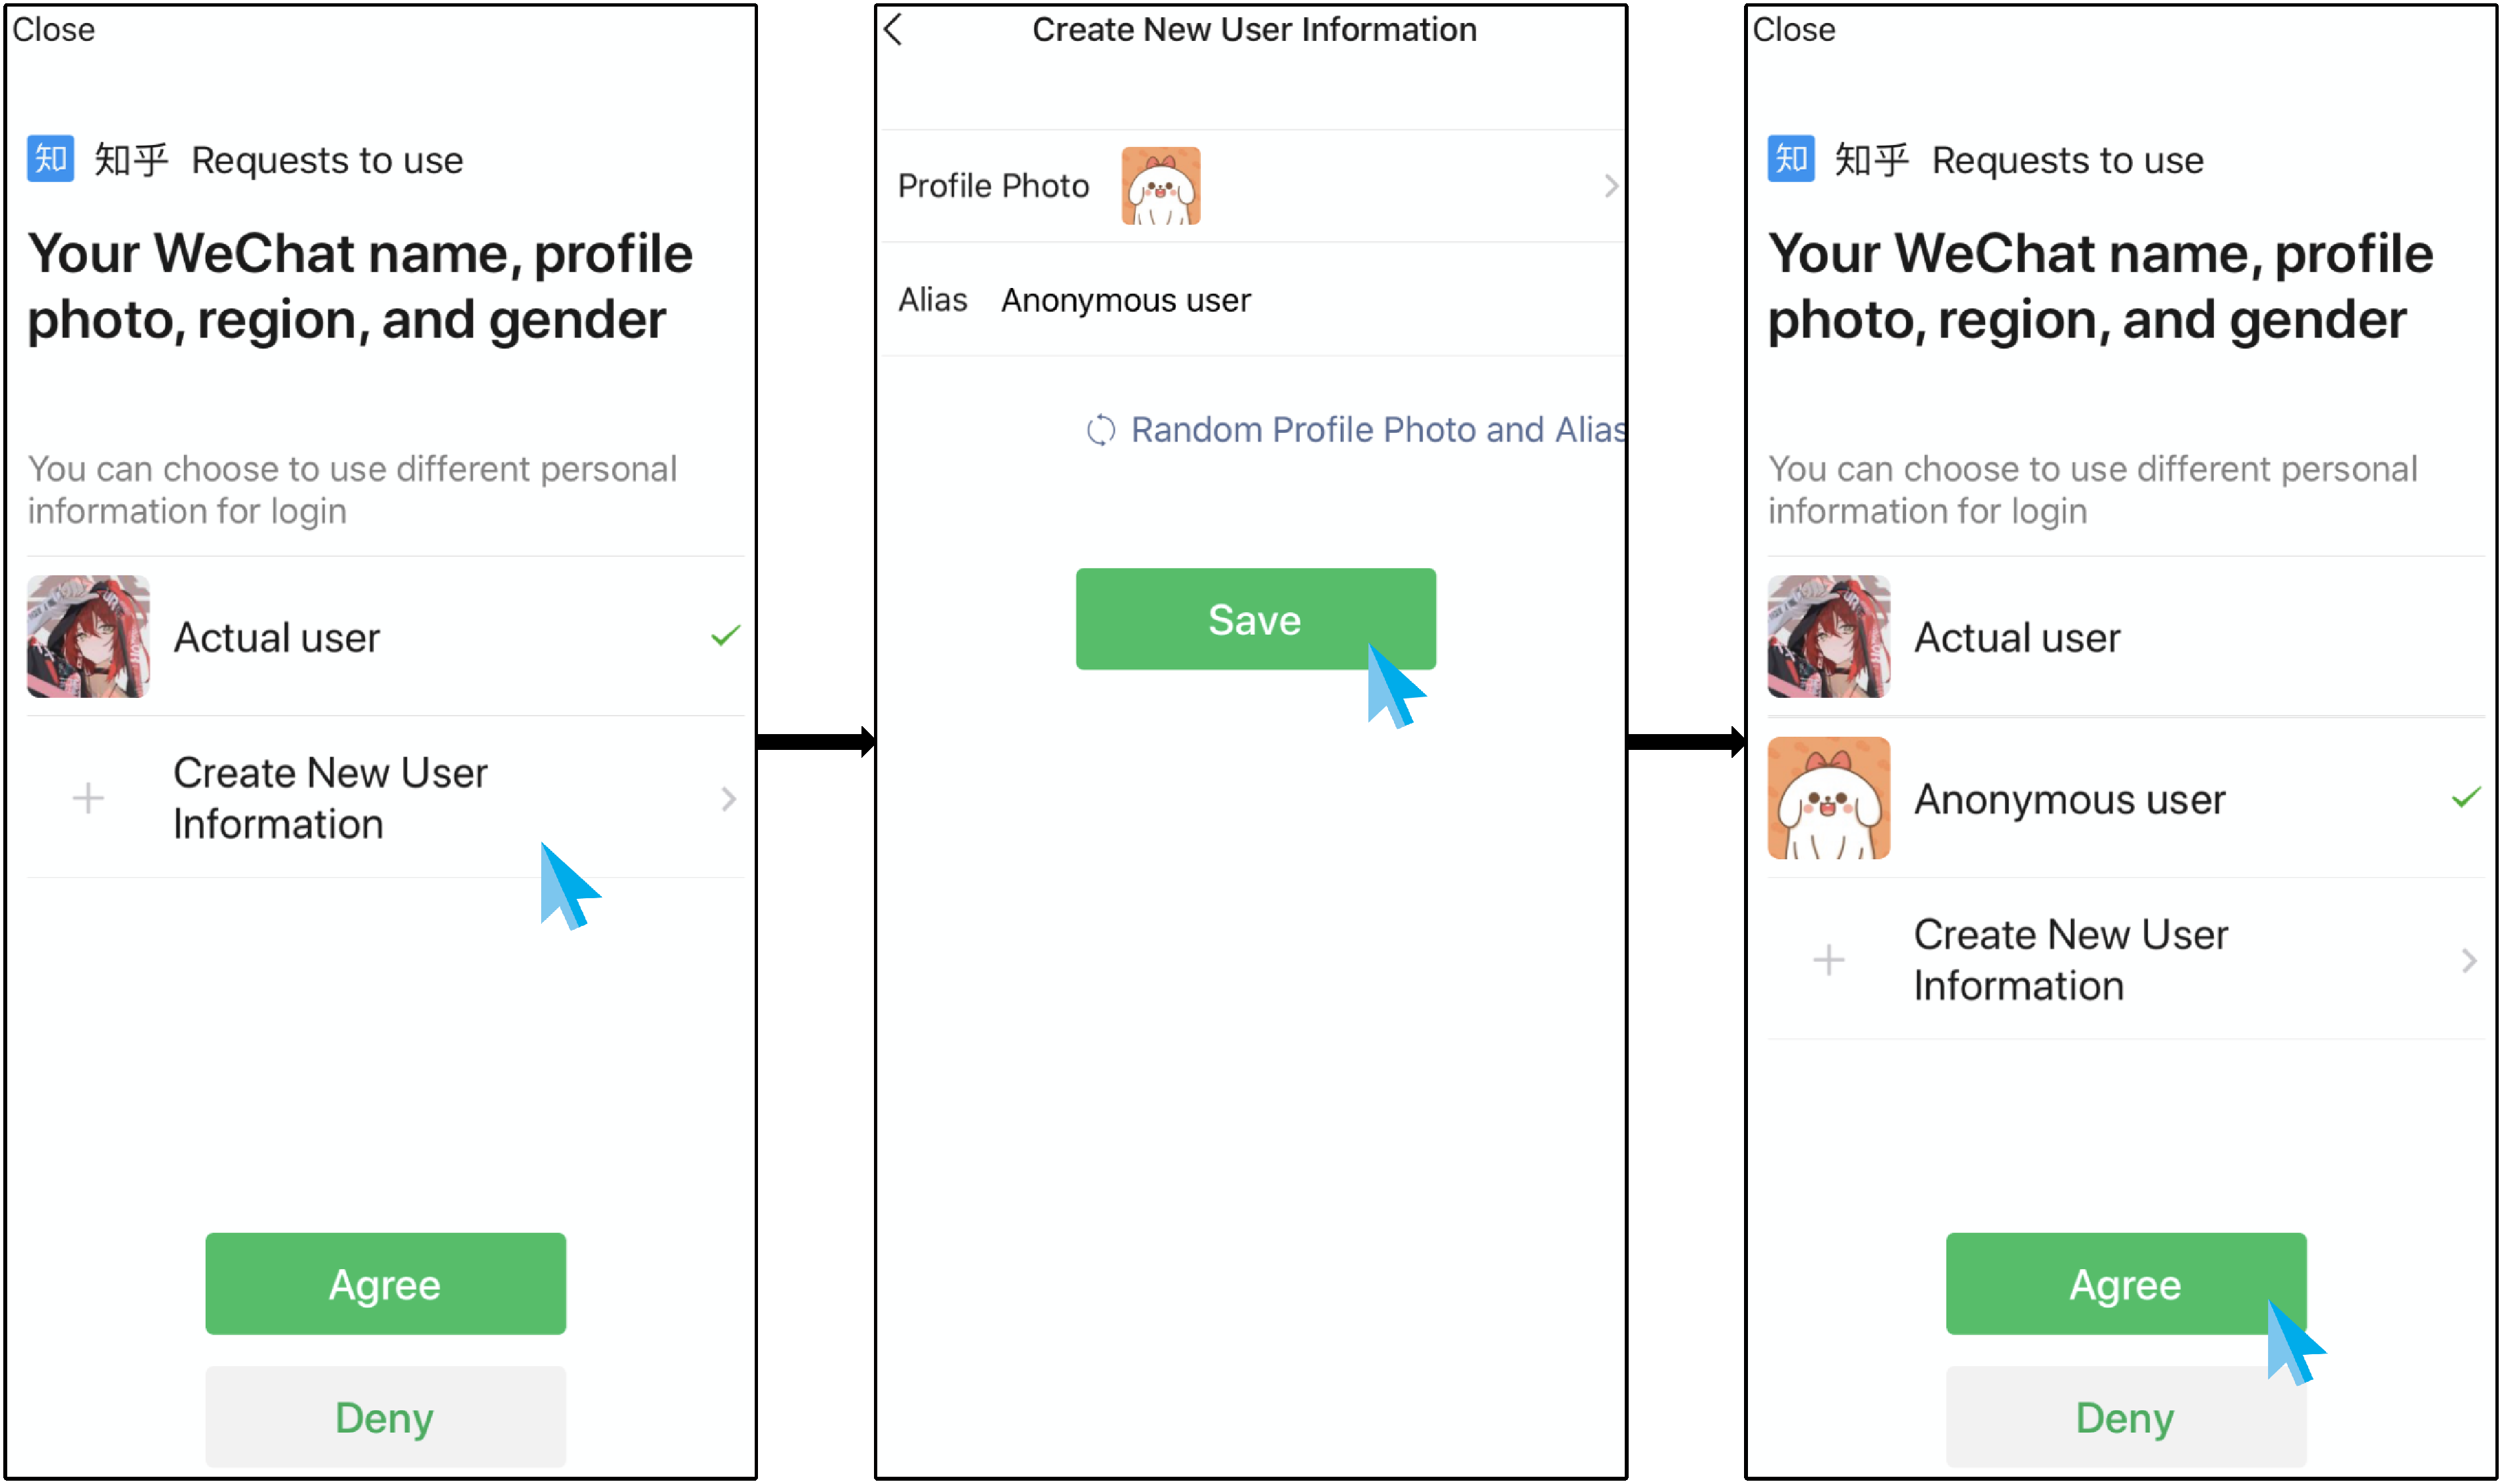
\includegraphics[width=0.9\linewidth]{fig/wechat.pdf}
%  \caption{Anonymous SSO login in WeChat.}
%  \label{fig:wechat}
%  \vspace{-5mm}
%\end{figure}

%also raises privacy concerns regarding online user tracking and profiling.
%Imagine that, a user concerning her privacy would avoid to leave her full sensitive information at an application. The user may use multiple web applications and only leave parts of her sensitive messages at each applications, for example, using  real name on social website, the address on shopping website and the phone number on Telecom website. And she would try not to leave any linkable message to avoid applications combining her informations, for example, if she leave the email on each applications, they can combine the parts of informations through the email. However,  the privacy leaks in SSO systems make her effort in vain. As long as a user employs the SSO system, such as Google Account, to log in to these applications, the applications providers and Google can combine your informations based on the SSO account.

%google and facebook�ĸ�������
%1. service provider����DNS��֪��������ˣ����Դ����ܶ����⡣���ǻ��Dz�ͬ�ģ�DNS��profile��Ҫ��������two behavior vectors��similarities����IdP�ж�����Ҫ����ΪIdP�ܹ�����two behavior vectors �Ƿ�������ͬ�ڵ㡣


Privacy-preserving SSO solutions try to provide comprehensive functions of identity management and authentication,
    while protecting user privacy \cite{maler2008venn,NIST2017draft,BrowserID,SPRESSO}.
The following features of SSO are usually supported:
(\emph{a}) \emph{User identity at an RP},
    i.e., an identity token enables an RP to uniquely identify every user,
(\emph{b}) \emph{Only user authentication to the IdP}, i.e.,
    the steps of user authentication between a user and the RP are eliminated,
    and a user only needs to hold the secret credential to authenticate himself to the IdP,
%    different types of credentials are supported in the authentication between the IdP and users,
and (\emph{c}) \emph{Provision of IdP-confirmed user attributes},
    i.e., a user maintains his attributes at the trusted IdP,
    and RP-requested attributes are provided with the user's identity
            after authorized by the user.
Meanwhile,
    the privacy threats from different types of adversaries are considered:
    (\emph{a}) \emph{the curious-but-honest IdP},
    (\emph{b}) \emph{collusive RPs},
    and (\emph{c}) \emph{the curious-but-honest IdP colluding some RPs}.
We analyze and compare existing privacy-preserving solutions of SSO and also federated identity management
in Section \ref{subsec-solutions}.


%However, to the best of our knowledge,
% {\em none of them provides a practical protection against both the IdP-based login tracing and the RP-based identity linkage}
%  (see Sections \ref{subsec-solutions} and \ref{sec:related} for details).
%The techniques proposed so far to defend against each of the two threats cannot be integrated,
%    for they require modifications to the SSO login flows that essentially conflicts.
%This requires a non-trivial re-design of SSO protocols against the threats of user privacy,
%while providing secure identity management and authentication.

We conceptualize the privacy requirements of SSO into
  an {\em identity transformation} problem, %and explain the reasons that limit existing solutions from fully protecting user privacy against both curious IdPs and collusive RPs.
and propose an Untraceable and Unlinkable Privacy-PREserving Single Sign-On (UPPRESSO) protocol
  to protect user privacy.
In particular, we design three identity-transformation functions in the SSO login flow.
In each login instance of UPPRESSO,
        $ID_{RP}$ is firstly transformed to an ephemeral $PID_{RP}$  cooperatively by the RP and the user.
Then, $PID_{RP}$ is sent to the IdP to transform $ID_U$ to ephemeral $PID_U$,
    so that the identity token binds $PID_U$ and $PID_{RP}$, instead of permanent $ID_U$ and $ID_{RP}$.
Finally,
    after receiving an identity token with matching $PID_{RP}$,
        the RP transforms $PID_U$ into an account.
Given a user, this account is (\emph{a}) identical across multiple login instances and (\emph{b}) unique at each RP.
UPPRESSO prevents the IdP from tracking a user's login activities because it receives only $PID_{RP}$ in the identity-token request,
    and collusive RPs from linking a user's identities across these RPs because every account is unique.
%This prevents both IdP-based login tracing by hiding the RPs' identities from the IdP and RP-based identity linkage by hiding the user's identity from the RPs.
%Meanwhile, an RP is still able to link multiple login sessions of the same user by converting the user's different pseudo-identities to an invariant user account using a special identifier-transformation function and the trapdoors, without knowing the user's real identity in the IdP.
% Finally, we formally prove that the accounts of the same user at different RPs are independent and cannot be correlated by collusive RPs (see our proof in Section \ref{sec:privacy}).
%UPPRESSO designs three one-way identifier-transformation functions based on elliptic curve cryptography. Using the one-way trapdoor function $\mathcal{F}_{ID_{RP} \mapsto PID_{RP}}(ID_{RP}, T)$, the RP converts its identity $ID_{RP}$ into a privacy-preserving pseudo-identity $PID_{RP}$ based on a randomly selected trapdoor $T$. Similarly, the IdP uses the one-way function  $\mathcal{F}_{ID_{U} \mapsto PID_{U}}(ID_U, PID_{RP})$ to generate a privacy-preserving pseudo-identity $PID_U$ for the user based on her identity $ID_U$ and $PID_{RP}$. Finally, using a special identifier-transformation function $\mathcal{F}_{PID_{U} \mapsto Account}(PID_U, PID_{RP}, T)$, the RP is able to map all the different privacy-preserving pseudo-identities of a user, which are created in her different login sessions to that RP, to a same $Account$ that identifies the user to the RP. The three identifier-transformation functions work cooperatively to ensure: (\emph{a}) when a user logs in to an RP multiple times, the RP can always map $PID_U$s to a unique $Account$ without knowing the user's identity $ID_U$; moreover, when a user logs in to multiple RPs, (\emph{b}) a curious IdP learns nothing about the identities of these RPs from $PID_{RP}$s, and (\emph{c}) collusive RPs cannot link $PID_U$s to a particular user %or associate them together, (\emph{d}) nor correlate $Account$s of a same user at different RPs.

While keeping the features of popular SSO,
UPPRESSO prevents both the IdP-based login tracing and the RP-based identity linkage,
    by the identity-transformation functions during the generation of identity tokens
    and the calculation of accounts.
The transformation functions work compatibly with
    the login flows of widely-used SSO protocols \cite{OpenIDConnect,rfc6749,SAML,NIST2017draft},
    so the benefits of SSO protocols are kept in UPPRESSO
        and it is very easy to implement UPPRESSO on top of OIDC systems.
%We do not solve the collusive attacks by the IdP and RPs.


We summarize our contributions as follows.
\begin{itemize}
\item We formalize the SSO privacy problems as an identity-transformation challenge,
    and
then propose a comprehensive solution to protect the users' login activities;
    that is, solve this challenge effectively by designing identity-transformation functions.
\item
The UPPRESSO protocol is then presented based on the identity transformations,
    with several designs specific for web applications.
We prove that UPPRESSO satisfies the security and privacy requirements of SSO services.

%To the best of our knowledge, UPPRESSO is the first practical SSO system against both the IdP-based login tracing and the RP-based identity linkage.

%\item We formally prove the privacy of UPPRESSO based on the DDH assumption \cite{GoldwasserK16} and the security of UPPRESSO based on a formal model of the web infrastructure. Our results show that UPPRESSO provides expected and satisfying security and privacy protection to SSO.
%provide the reduction from UPPRESSO scheme to DDH Assumption proving that it is protected from IdP-based login tracing and RP-based identity linkage,
%and analyze the security of UPPRESSO based on a formal model of the web infrastructure and formally prove that it provides satisfying security properties.
\item
We build the UPPRESSO prototype system for web applications,
    on top of an open-source OIDC implementation.
The experimental performance evaluations show that UPPRESSO introduces reasonable overheads.
\end{itemize}

%The remainder is organized as follows.
Section \ref{sec:background} presents
    the background and related works.
The identity dilemma of privacy-preserving SSO is analyzed  in Section \ref{sec:challenge},
    and Section \ref{sec:UPPRESSO} presents the detailed designs of UPPRESSO.
The properties of security and privacy are analyzed in Section \ref{sec:analysis}.
We explain the prototype implementation and experimental evaluations in Section \ref{sec:implementation},
 and discuss extended issues in Section \ref{sec:discussion}.
Section \ref{sec:conclusion} concludes this work.


%\section{Background and Related Works}
\label{sec:background}
%UPPRESSO is designed to be compatible with OpenID Connect (OIDC) and provide privacy protections based on the discrete logarithm problem. Next,

We introduce %OIDC \cite{OpenIDConnect}, to describe
  typical SSO login flows,
 and discuss existing privacy-preserving solutions and other related works.

\subsection{OpenID Connect and SSO Services}
\label{subsec:OIDC}
OIDC is one of the most popular SSO protocols. % for web applications. %As other SSO protocols \cite{SAMLIdentifier}, OIDC
%It involves three entities, i.e., {\em users}, the {\em identity provider (IdP)}, and {\em relying parties (RPs)}.
Users and RPs initially register at the IdP with their identities %($ID_U$, $ID_{RP}$ and $PID_U$ in some schemes) %(or $PID_{RP}$ in some schemes)
and other necessary information such as user credentials %(i.e., passwords or key pairs)
 and RP endpoints (i.e., the URLs to receive identity tokens).
% below can be removed
%The IdP should maintain these attributes securely.

%\vspace{1mm}
%\noindent\textbf{Implicit Login Flow.}
OIDC supports three types of login flows: implicit flow, authorization code flow, and hybrid flow (i.e., a mix-up of the other two).
%In the implicit flow, an {\em id token} is generated as the identity token, which contains a user identifier, an RP identifier, the issuer (i.e., IdP), the validity period, and other requested attributes. The IdP signs the id token using its private key to ensure integrity, and sends it to the RP through the user.
%In the authorization code flow, the IdP binds an authorization code with the RP, and sends it to the RP through the user; then, the RP establishes an HTTPS connection to the IdP and uses the authorization code with the RP's credential to obtain the user's identifier and other attributes.
%UPPRESSO is compatible with all three flows.
They work with different steps to request and receive identity tokens,
    but with the common security requirements of identity tokens.
We introduce the implicit flow and present our designs based on this flow.
Section \ref{sec:discussion} discusses the supports of authorization code flows.

\begin{figure}[t]
  \centering
  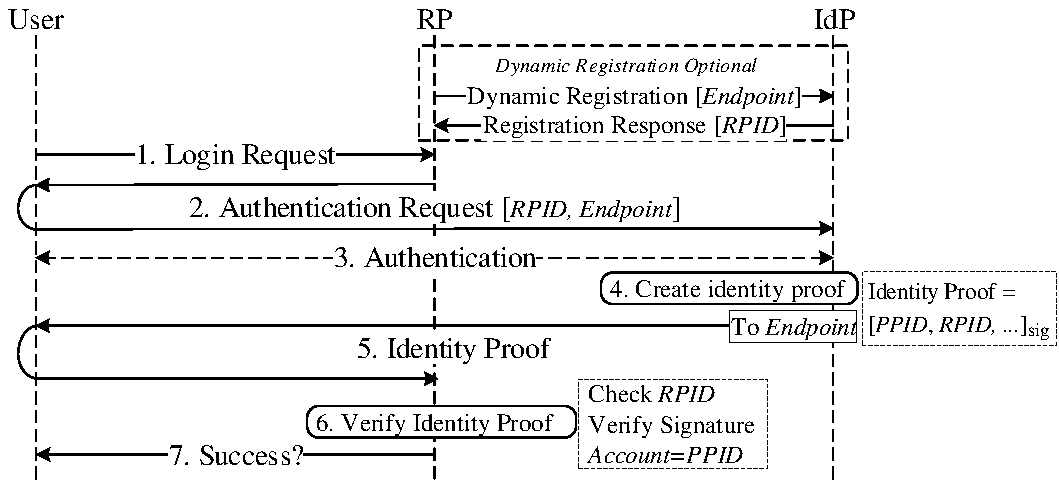
\includegraphics[width=0.9\linewidth]{fig/OIDC1.pdf}
  \caption{The implicit SSO login flow of OIDC.}
  \label{fig:OpenID}
%  \vspace{-5mm}
\end{figure}

As shown in Figure \ref{fig:OpenID}, a user firstly initiates a login request to an RP.
Then, the RP constructs an identity-token request with its own identity
 and the scope of requested user attributes.
This request is redirected to the IdP.
After authenticating the user,
    the IdP issues an identity token
        which is forwarded by the user to the RP endpoint.
The token contains a user identity (or pseudo-identity),
    the RP identity, a validity period, the requested user attributes, etc.
Finally, the RP verifies the received identity token and
 allows the user to login as the  enclosed (pseudo-)identity.
The user's operations including redirection, authorization, and forwarding,
    are implemented in a software called user agent (i.e., a browser).

%Before issuing the identity token,
%    the IdP obtains the user's authorization to enclose the requested attributes.
 %   which are maintained at the IdP by the user.
%The IdP is also a web service.
%The identity token is usually signed by the IdP,
%    and transmitted through secure channels such as TLS/HTTPS.

%extracts user's identifier and returns the authentication result to the user (Step 7).


\begin{table*}[tb]
\footnotesize
    \caption{Privacy-Preserving Solutions of SSO and Identity Federation.}
    \centering
    \begin{tabular}{|c|c|c|c|c|c|c|}
  \hline
  \multirow{3}*{\textbf{~~Solution~~}} &
  \multicolumn{3}{c|}{\textbf{SSO Feature} - supported $\CIRCLE$, unsupported $\Circle$, or partially $\LEFTcircle$} & \multicolumn{3}{c|}{\textbf{Privacy Threat} - prevented $\CIRCLE$ or not $\Circle$} \\ \cline{2-7}
  & User Identity & User Authentication & IdP-Confirmed Selective  & IdP-based & RP-based & Collusive Attack \\
  & at an RP & Only to the IdP &  Attribute Provision & Login Tracing & Identity Linkage & by the IdP and RPs \\\hline\hline
  OIDC with PPID \cite{NIST2017draft} & $\CIRCLE$ & $\CIRCLE$ & $\CIRCLE$ & $\Circle$ & $\CIRCLE$ & - \\ \hline
  BrowserID \cite{BrowserID} & $\CIRCLE$ & $\LEFTcircle$$^1$ & $\Circle$ & $\CIRCLE$ & $\Circle$ & - \\ \hline
  SPRESSO \cite{SPRESSO} & $\CIRCLE$ & $\CIRCLE$ & $\Circle$$^2$ & $\CIRCLE$ & $\Circle$ & - \\ \hline
  PRIMA \cite{prima} & $\CIRCLE$ & $\Circle$ & $\CIRCLE$ & $\CIRCLE$ & $\Circle$ & - \\ \hline
  PseudoID \cite{PseudoID} & $\CIRCLE$ & $\Circle$ & $\Circle$$^3$ & $\CIRCLE$ & $\CIRCLE$ & $\CIRCLE$ \\ \hline
  EL PASSO \cite{ELPASSO} & $\CIRCLE$ & $\Circle$ & $\CIRCLE$ & $\CIRCLE$ & $\CIRCLE$ & $\CIRCLE$ \\ \hline
  UnlimitID \cite{UnlimitID} & $\CIRCLE$ & $\Circle$ & $\CIRCLE$ & $\CIRCLE$ & $\CIRCLE$ & $\CIRCLE$ \\ \hline
  Opaak \cite{Opaak} & $\LEFTcircle$$^4$ & $\Circle$ & $\Circle$ & $\CIRCLE$ & $\CIRCLE$ & $\CIRCLE$ \\ \hline
  Fabric Idemix \cite{hyperledge-idemix} & $\Circle$$^5$ & $\Circle$ & $\CIRCLE$ & $\CIRCLE$ & $\CIRCLE$ & $\CIRCLE$ \\ \hline
  U-Prove \cite{uprov} & $\CIRCLE$ & $\Circle$ & $\LEFTcircle$$^6$ & $\CIRCLE$ & $\CIRCLE$ & $\CIRCLE$ \\ \hline
  UPPRESSO & $\CIRCLE$ & $\CIRCLE$ & $\CIRCLE$ & $\CIRCLE$ & $\CIRCLE$ & $\Circle$ \\ \hline
\end{tabular}
    \label{tbl:comparison-protocol}
\flushleft
{\footnotesize
1. A BrowserID user generates an \emph{ephemeral} private key to sign every ``subsidiary'' token,
 which is verified by the RP.\\
2. SPRESSO can be extended to provide user attributes in then tokens, while the prototype does not support it.\\
3. Blindly-signed user attributes can be selectively provided using zero-knowledge proofs,
    but not implemented in the prototype \cite{PseudoID}.\\
4. Opaak supports exclusive pseudonym options: (\emph{a}) linkable within an RP but unlinkable across multiple RPs and (\emph{b}) unlinkability for any two actions.\\
5. In the original design of Idemix \cite{idemix}, every user logins to an RP with a unique account.\\
6. A U-Prove token may contain some attributes \emph{invisible} to the IdP, in addition the ones confirmed by the IdP.}
\end{table*}


The following features are supported in widely-used popular SSO solutions \cite{NIST2017draft,OpenIDConnect,rfc6749,SAML,SAMLIdentifier}.
\\\textbf{User Identity at an RP.}
The identity tokens facilitate the target RP to identify each user as a unique account at this RP,
    and this account links the user's multiple login instances to this RP
        for customized services.
%On the contrary, in anonymous SSO systems \cite{WangWS13,HanCSTW18,HanCSTWW20}
%        the RP only verifies whether he is a legitimate user authenticated by the IdP
%            and receives no information to distinguish every user.
\\\textbf{User Authentication Only to the IdP.}
A ``pure'' SSO protocol  \cite{OpenIDConnect,rfc6749,SAML} does not include authentication steps:
    the authentication between a user and the IdP is conducted independently.
This
    enables the IdP to authenticate users by any appropriate means (e.g., password,
one-time password, and multi-factor authentication).
It eliminates the authentication steps between users and an RP,
        and RPs only verify tokens issued by the IdP.
A user holds only the credential to authenticate himself to the IdP,
    and the burden is greatly reduced.
If this credential was lost or leaked,
    the user only renews it at the IdP.
However, if a user proves some non-ephemeral secret to RPs and this secret is valid across multiple login instances
    (i.e., authentication steps are actually involved),
                the user has to notify each RP if it was leaked. %during its validity period. %(or even the user logins from another computer).
\\\textbf{IdP-Confirmed Selective Attribute Provision.}
The IdP usually provides user attributes in the tokens \cite{OpenIDConnect,rfc6749,SAML},
    in addition to user (pseudo-)identities.
These attributes are maintained by users at the IdP.
%    for example,
%        when Facebook provides social networking services,
%         it also issues identity tokens enclosing user identities and various attributes.
Before enclosing attributes in a token,
    the IdP obtains the user's authorization;
    or the provided attributes are selected by the user.
So no distinctive attributes such as telephone number, Email address, etc.,
        are enclosed in the identity tokens of privacy-preserving SSO systems.

%\vspace{1mm}
%\noindent\textbf{RP Dynamic Registration.}
%In addition to manual registrations,
%    OIDC also supports dynamic registrations
%    for an RP to register by online means \cite{DynamicRegistration}.
%The (unregistered) RP sends a registration request
%        with endpoints to receive identity tokens (and other information),
%        to the IdP.
%After a successful registration,
% the IdP assigns a unique RP identity in the response.
%

%UPPRESSO leverages this function and slightly modifies the dynamic registration process to implement the {\em $PID_{RP}$ registration} process (see details in Section \ref{sec:UPPRESSO}.C), which allows an RP to generate different privacy-preserving RP identifiers and register them with the IdP.


\subsection{Privacy-Preserving SSO and Identity Federation}
\label{subsec-solutions}
Table \ref{tbl:comparison-protocol} lists privacy-preserving solutions of SSO and identity federation.
Widely-used SSO protocols \cite{OpenIDConnect,rfc6749,SAML,SAMLIdentifier} allow a user to login to RPs,
%    after being authenticated by the IdP,
        without by himself holding any permanent secret verified by RPs
        or maintain accounts for these RPs.
While keeping this user convenience,
 existing privacy-preserving SSO \cite{BrowserID,SPRESSO,NIST2017draft} prevents the IdP-based login tracing or the RP-based identity linkage,
    and UPPRESSO prevents both of them.

Identity federation enables a user registered at the IdP to be accepted by other parties,
            with different accounts sometimes,
        but more user operations are involved than those of SSO.
Privacy-preserving identity federation \cite{ELPASSO,UnlimitID,hyperledge-idemix,PseudoID,Opaak}
    protects privacy against even collusive attacks by the IdP and the RPs,
    but requires a user to (\emph{a}) hold long-term secrets verified by RPs,
            in addition to the authentication credentials for the IdP,
                and (\emph{b}) manage the accounts at different RPs by himself.
That is, there are actually some authentication steps between the user and RPs (or called asynchronous authentication \cite{ELPASSO}).


Pairwise pseudonymous identifiers (PPIDs) are recommended \cite{NIST2017draft}
 and specified in SSO protocols \cite{OpenIDConnect, SAMLIdentifier} to protect user privacy against curious RPs.
When issuing an identity token,
        the IdP encloses a user PPID (but not the identity at the IdP).
Given a user,
    the IdP assigns a unique PPID based on the target RP,
    so collusive RPs cannot link the users.
PPIDs cannot prevent the IdP-based login tracing,
 for the IdP needs the RP identity to issue tokens.



Some solutions prevent the IdP-based login tracing,
    but vulnerable to the RP-based identity linkage.
In BrowserID \cite{BrowserID} (formerly known as Firefox Accounts \cite{FirefoxAccount} and Mozilla Persona \cite{persona}),
 the IdP %(called the primary identity authority in BrowserID)
  issues a special token (called user certificate) to bind a user identity to an \emph{ephemeral} public key,
 so the user utilizes the private key to sign a ``subsidiary'' token (called identity assertion)
    to bind the target RP's identity and sends both tokens to the RP.
The PRIMA IdP signs a credential binding a verification key and a set of user attributes \cite{prima}, and the key is viewed as the user identity.
The user selectively provides IdP-confirmed attributes to an RP using his signing key \cite{Oblivion}. % cooperatively with the IdP.
In SPRESSO \cite{SPRESSO} an RP assigns a verifiable one-time pseudo-identity to itself in each login instance.
Then, the IdP generates an identity token binding this RP pseudo-identity. %and the user identity.
In these schemes \cite{BrowserID,prima,SPRESSO}
    collusive RPs could link a user based on his unique identity in the tokens (or credentials).


PseudoID \cite{PseudoID} introduces an independent token service in addition to the IdP,
    to  \emph{blindly} sign an access token binding a pseudonym and a user secret.
The user unblinds this token,
 and the IdP will assert it,
    which allows the user to login to an RP using his secret.
Two kinds of privacy threats are prevented, because (\emph{a}) the RP's identity is not enclosed in the access token
    and (\emph{b}) the user encloses different pseudonyms when visiting RPs.
Collusive attacks by the IdP and RPs are also prevented,
    for they cannot link two blindly-signed tokens.

% the user must use the secret to login to RP, because no RP identity is enclosed in the token.


%However, the user has to permanently keep the secret preimage for each account in an RP.

In EL PASSO \cite{ELPASSO}, after authenticating a user,
    the IdP signs an anonymous credential \cite{anon-credential} binding a secret,
         both of which are kept on the user's device.
When attempting to login to an RP,
    the user proves that he is the owner of this credential without exposing the secret,
        and discloses selective attributes in the credential.
Although one credential is proved to multiple RPs,
        user-maintained pseudonyms and anonymous credentials prevent the RPs, even when collusive with the IdP, from linking the users across the RPs.
UnlimitID \cite{UnlimitID} presents similar designs based on anonymous credentials \cite{anon-credential},
        to prevent collusive attacks by the IdP and RPs.
NEXTLEAP \cite{nextleap} adopts UnlimitID for anonymous secure messaging.

%    but a user has to by himself manage pseudonyms for different RPs.
%For example,
%    the RP domain (e.g., \verb+www.RP.com+) is used as a factor to locally generate the user's account (or pseudonym) at this RP.

Anonymous credentials \cite{anon-credential-2001,anon-credential} are utilized in flexible ways.
Opaak \cite{Opaak} keeps IdP-signed anonymous credentials in mobile phones as pseudonym tokens,
    which bind a user's secret key.
The Idemix anonymous credential system \cite{idemix}
 is integrated in Hyperledger Fabric \cite{hyperledge-idemix} to implement completely-unlinkable pseudonyms
        and IdP-confirmed selective attribute disclosure.
After a user retrieves a U-Prove token \cite{uprov,uprove-conference} from the IdP,
    it enables the user to authenticate himself and selectively disclose attributes to an RP.


%\section{The Identity-Transformation Framework}
%\section{The Identifier-Transformation Approach of UPPRESSO}
\label{sec:challenge}

This section investigates the security and privacy requirements of SSO,
    and explains the identity dilemma of privacy-preserving SSO.
Then,
    we present the identity-transformation framework which helps to design UPPRESSO.
%Finally, this framework is applied to analyze existing privacy-preserving SSO systems.

\subsection{Security Requirements of SSO}
\label{subsec:basicrequirements}
%A dedicated, the bidirectional authenticated secure channel was proposed to improve the confidentiality and integrity of identity token \cite{CaoSBKVC14}.

The primary goal of non-anonymous SSO services is secure user authentication \cite{SPRESSO},
 to ensure that a \emph{legitimate} user can always login to an \emph{honest} RP as his permanent identity at this RP, %correlating multiple login instances,
    by presenting the \emph{identity tokens} issued by the \emph{honest} IdP.

To achieve this goal,
 an identity token generated by the IdP is required to specify (\emph{a}) the RP to which the user requests to login (i.e., \emph{RP designation})
    and  (\emph{b}) exactly the user who is authenticated by the IdP (i.e., \emph{user identification}).
Accordingly,
    an honest RP verifies the designated RP identity (or pseudo-identity) in identity tokens with its own before accepting the tokens;
     otherwise,
        a malicious RP could replay a received identity token to the honest RP and login as the victim user.
The RP allows the token holder to login as the user identity (or pseudo-identity) specified in the accepted tokens;
    otherwise, the IdP provides only anonymous services.

The SSO login flow implies \emph{confidentiality} and \emph{integrity} of identity tokens.
An identity token shall be forwarded by the authenticated user to the target RP only,
    not leaked to adversaries;
        otherwise, an adversary who presents the token, would successfully login to this honest RP.
Integrity is necessary,
    to prevent adversaries from tampering with an identity token,
        without being detected by the RPs.
So identity tokens are signed by the IdP and usually transmitted over HTTPS.

These four security requirements (i.e., RP designation, user identification, confidentiality, and integrity) of SSO identity tokens
     have been discussed and analyzed \cite{ArmandoCCCT08,FettKS16, FettKS17},
     and
     any vulnerabilities breaking one or more of these properties in SSO systems
            result in effective attacks \cite{SomorovskyMSKJ12, WangCW12, ArmandoCCCPS13, ZhouE14, WangZLLYLG15, WangZLG16, YangLLZH16, MainkaMS16, MainkaMSW17, YangLCZ18, YangLS17, ShiWL19, ChenPCTKT14, ccsSunB12, DiscoveringJCS, dimvaLiM16, CaoSBKVC14, TowardsShehabM14}.
An adversary might attempt to login to an honest RP as a victim user (i.e., \emph{impersonation}),
 or allure a victim user to login to an honest RP as the attacker (i.e.,  \emph{identity injection}).
For example, Friendcaster used to accept any received identity token, which violates RP designation \cite{ChenPCTKT14},
    so a malicious RP could replay a received identity token to Friendcaster and login as the victim user.
The defective IdP of Google ID SSO signs identity tokens where the Email element was not enclosed,
        while some RPs use a user's Email as his unique username \cite{WangCW12}.
So this violation of user identity resulted in vulnerable services.
Because identity tokens were leaked in different ways \cite{WangCW12,ccsSunB12,ArmandoCCCPS13,DiscoveringJCS,dimvaLiM16},
 the eavesdroppers could impersonate the victim users.
Some RPs even accept user attributes that are not bound in identity tokens (i.e., a violation of integrity) \cite{WangCW12},
  so that adversaries could insert arbitrary attributes into the identity tokens to impersonate another user at these RPs.


\begin{comment}
We summarize the basic requirements of SSO systems based on existing theoretical analyses \cite{ArmandoCCCT08,FettKS16, FettKS17} and practical attacks \cite{SomorovskyMSKJ12,WangCW12,ArmandoCCCPS13,ZhouE14,WangZLLYLG15,WangZLG16,YangLLZH16,MainkaMS16,MohsenS16,MainkaMSW17,YangLCZ18,YangLS17,ShiWL19}. These requirements enable an SSO system to provide qualified authentication services for RPs, through identity tokens.
\begin{itemize}
\item \textbf{User identification.} When a user logs into a certain RP for multiple times by submitting identity tokens, the RP extracts the identical user identifier from these identity tokens, to provide personalized services for this user.
\item \textbf{RP designation.} The designated receiver (or RP) is specified in an identity token, so that this identity token is accepted by the visited RP only.
\item \textbf{Integrity and confidentiality.} Only the IdP is trusted to generate identity tokens, RPs do not accept an identity token with any modification or a forged one. %RPs should only accept the valid identity token.
Meanwhile, a valid identity token is transmitted only to the user and the designated RP. % confidentiality of the identity token is ensured during the transmission among the IdP, user and the designated RP.
\end{itemize}

%These basic requirements are the minimum properties that an SSO system has to provide.
% therefore RPs should be able to identify the user with the help from IdP.
First of all, user identification is necessary for common SSO systems to help the RPs to receive the user's identifier, except the anonymous services.
Any violation of these requirements \cite{SomorovskyMSKJ12,WangCW12,ArmandoCCCPS13,ZhouE14,WangZLLYLG15,WangZLG16,YangLLZH16,MainkaMS16,MohsenS16,MainkaMSW17,YangLCZ18,YangLS17,ShiWL19} result in \emph{impersonation attacks} (i.e., the adversaries log into an honest RP as a victim user) or \emph{identity injection attacks} (i.e., a victim user logs into an honest RP under some attacker's identity).
% and without integrity, the impersonation and identity injection attacks could be constructed easily
% as an adversary could directly modify user's identifier in the identity token;
If the designated RP is not well specified or verified in identity tokens, the adversaries could deceive an RP to accept the identity tokens generated for other RPs, so that the adversaries would (\emph{a}) impersonate some victim user, by colluding with a malicious RP to obtain such an identity token and submitting it to the RP, or (\emph{b}) inject such identity tokens in the communications between the victim user and some RP.
   %                  for example, by CSRF \cite{zeller2008cross}.
Impersonation and identity injection attacks would be successfully launched, if the attackers could arbitrarily modify the user identifiers in identity tokens.
Or, the adversaries could impersonate the victim user by submitting any leaked identity token to the RP \cite{ChenPCTKT14,FettKS16,WangZLG16}, if confidentiality is not well ensured.

The design and implementation of a secure SSO system is challenging, while various vulnerabilities have been found and exploited to break at least one requirement \cite{ChenPCTKT14, FettKS16,WangCW12,ZhouE14,WangZLG16,YangLLZH16,SomorovskyMSKJ12,MohsenS16}.
For example, Friendcaster was found to accept any received identity token \cite{ExplicatingSDK,ChenPCTKT14}
(i.e., a violation of RP designation) so that a malicious RP could log into Friendcaster as the victim user by replaying the identity token received from the user to Friendcaster \cite{MohsenS16}. \cite{WangCW12} reported that some RPs of Google ID SSO accepted user attributes that were not tied to the identity token (i.e., a violation of integrity). As a result, a malicious user could insert arbitrary attributes (e.g., an email address) into the identity token to impersonate another user at the RP.
\end{comment}


\subsection{The Identity Dilemma of Privacy-Preserving SSO}
\label{subsec:challenges}
A \emph{completely} privacy-preserving SSO system shall offer the four security properties as mentioned above,
    while prevent the privacy threats due to the IdP-based login tracing and the RP-based identity linkage.
However, to satisfy the requirements of security and privacy at the same time,
     poses a dilemma in the generation of identity tokens as follows.
Table \ref{tbl:notations-dilemma} lists the notations used in the following explanation,
    and the subscript $j$ and/or the superscript $i$ may be omitted sometimes, when there is no ambiguity.

\begin{table}[t]
\footnotesize
    \caption{The (pseudo-)identities in privacy-preserving SSO.}
    \centering
%    \begin{tabular}{|l|l|l|}
    \begin{tabular}{|p{1.0cm}|p{5.1cm}|p{1.13cm}|} \hline
    {\textbf{Notation}} & {\textbf{Description}} & {\textbf{Attribute}} \\ \hline
    {$ID_U$} & {The user's unique identity at the IdP.} & {Permanent} \\ \hline
    {$ID_{RP_j}$} & {The $j$-th RP's unique identity at the IdP.} & {Permanent} \\ \hline
    {$PID_{U,j}^i$} & {The user's pseudo-identity, in the user's $i$-th login instance to the $j$-th RP.} & {Ephemeral} \\ \hline
    {$PID_{RP_j}^i$} & {The $j$-th RP's pseudo-identity, in the user's $i$-th login instance to this RP.} & {Ephemeral} \\ \hline
    {$Acct_j$} & {The user's identity (or account) at the $j$-th RP.} & {Permanent} \\ \hline
    \end{tabular}
    \label{tbl:notations-dilemma}
\end{table}


A valid identity token contains the identities (or pseudo-identities) of the authenticated user and the target RP. %which is to tell the RP that this user has been authenticated by the IdP.
% Let us denote the long-term unique identifiers of the user and the RP as $ID_U$ and $ID_{RP}$, respectively.
Since the IdP authenticates users and always knows the user's identity (i.e., $ID_U$),
    in order to prevent the IdP-based login tracing,
    we shall not reveal the target RP's permanent identity (i.e., $ID_{RP}$) to the IdP in the login flow.
So an \emph{ephemeral} pseudo-identity for the RP (i.e., $PID_{RP}$) shall be used in the communications with the IdP:
(\emph{a}) to ensure RP designation,
     $PID_{RP}$ shall be uniquely associated with the target RP;
    and (\emph{b}) the IdP cannot derive any information about $ID_{RP}$ from any $PID_{RP}^i$,
        which implies $PID_{RP}^i$ in multiple login instances shall
         be independent of each other.\footnote{Even when the target RP is kept unknown to the IdP,
            the IdP shall not link multiple login instances which attempt to visit this RP.}
   % the IdP-based login tracing is still effective, to correlate a user's multiple login instances.

Next, in order to prevent the RP-based identity linkage,
 the IdP shall not directly enclose $ID_U$ in identity tokens.
A pseudo-identity for the user (i.e., $PID_U$) shall be bound instead:
    (\emph{a}) the RP cannot derive any information about $ID_U$ from any $PID_{U,j}$,
    which implies $PID_{U,j}$ for different RPs shall be independent of each other;
    (\emph{b}) in multiple login instances to the RP, $PID_U^i$ shall be independent of each other or generated ephemerally,
        to prevent the IdP-based login tracing;\footnote{If $PID_U^i$ is not completely independent of each other,
         it implies the IdP could link multiple login instances which attempt to visit this RP.}
    and (\emph{c}) to ensure user identification,
    an \emph{ephemeral} $PID_{U}^i$ in each login instance shall facilitate the RP to correlate it
     with the \emph{permanent} account (i.e., $Acct$) at this RP.


We summary these identities and pseudo-identities.
That is,
    (\emph{a}) an identity tokens shall contain only the pseudo-identities, i.e., $PID_{U,j}^i$ and $PID_{RP_j}^i$,
        which are independent of each other for different RPs and in multiple login instances, respectively,
    and (\emph{b}) these two \emph{ephemeral} pseudo-identities enable the RP to calculate the \emph{permanent} account, i.e., $Acct_j$.

We illustrate the relationships among the identities and pseudo-identities in identity tokens in Figure \ref{fig:IDCorrelation}.
The red and green blocks represent permanent identities and ephemeral pseudo-identities, respectively.
The arrows denote how the pseudo-identities are transformed.
The figure describes the {\em identity dilemma} of privacy-preserving SSO:
\begin{quote}
Given an authenticated user and an unknown RP (i.e., permanent $ID_U$ and ephemeral $PID_{RP}$),
    the IdP is expected to generate an ephemeral pseudo-identity (i.e., $PID_{U}$)
     which will be correlated with the user's permanent identity at this RP (i.e., $Acct$),
     with knowing nothing about the RP's identity or the user's account at this RP (i.e., $ID_{RP}$ or $Acct$).
\end{quote}

\emph{We explicitly distinguish a user's identity at the RP, i.e., the account,
     from \emph{(a)} the user's identity at the IdP and \emph{(b)} the user's pseudo-identity in identity tokens.}
This conceptualization is proposed for the first time, to the best of our knowledge,
    and it essentially helps to effectively build the identity-transformation framework.


\begin{figure}
  \centering
  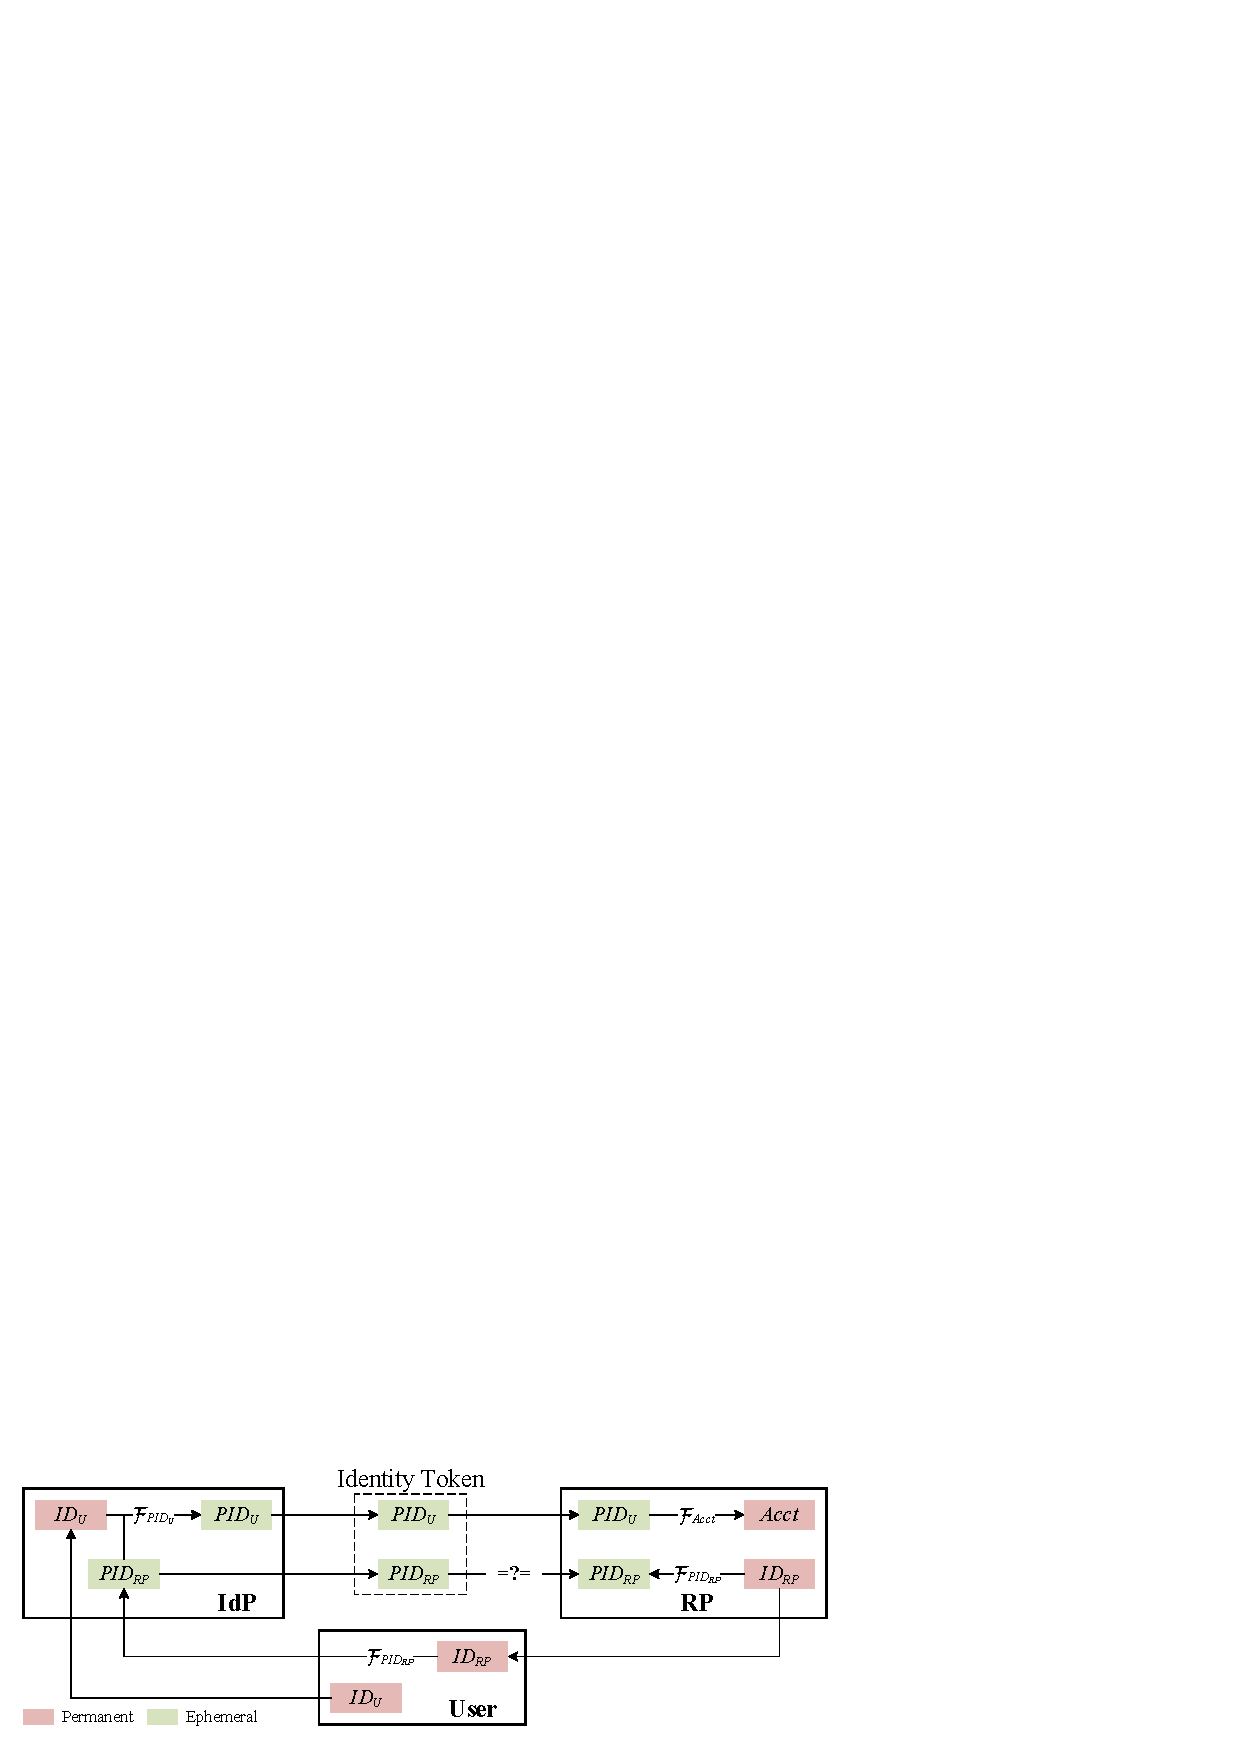
\includegraphics[width=0.98\linewidth]{fig/IDCorrelation.pdf}
  \caption{Identity transformations in privacy-preserving SSO.}
  \label{fig:IDCorrelation}
\end{figure}

\subsection{Identity Transformation}
\label{subsec:solutions}

%In the identity dilemma, we explicitly separate a user's account at the RP
%     from the user's unique identity at the IdP and the user's  pseudo-identity in identity tokens.
%This method guides us to propose the identity-transformation framework
%    (and then to solve the identity dilemma).


%we should provide the IdP some information related to the user's $Account$ at the RP to assist the generation of $PID_U$,
% so that $PID_U$ can be correctly correlated with the $Account$. Meanwhile, such information should not provide any additional knowledge for the IdP to derive the RP's identity, or for two RPs to correlate two $Account$s belonging to the same user.
The privacy-protection problem of SSO is converted into an identity-transformation challenge,
 to design three \emph{identity-transformation functions} as follows.
\begin{itemize}
\item
$\mathcal{F}_{PID_{RP}}(ID_{RP}) = PID_{RP}$, calculated by the user and/or the RP.
From the IdP's view,
$\mathcal{F}_{PID_{RP}}()$ is a one-way function and the calculated $PID_{RP}$ appears a random variable.
\item
$\mathcal{F}_{PID_U}(ID_U, PID_{RP}) = PID_{U}$, calculated by the IdP.
From the RP's view,
    $\mathcal{F}_{PID_U}()$ is a one-way function and the calculated $PID_{U}$ appears a random variable.
\item
$\mathcal{F}_{Acct}(PID_{U}, PID_{RP}) = Acct$, calculated by the RP.
Given $ID_U$ and $ID_{RP}$, $Acct$ keeps unchanged;
    i.e., in the user's any $i$-th and $i'$-th ($i \neq i'$) login instances to the RP,
 $\mathcal{F}_{Acct}(PID_{U}^i, PID_{RP}^i) = \mathcal{F}_{Acct}(PID_{U}^{i'}, PID_{RP}^{i'})$.
\end{itemize}


In an SSO login flow with identity-transformation functions,
    a user firstly negotiates an ephemeral $PID_{RP}$ with the target RP.
Then, an identity-token request with $PID_{RP}$ is sent by the user to the IdP.
After authenticating the user as $ID_U$, the IdP calculates an ephemeral $PID_U$ based on $ID_U$ and the received $PID_{RP}$,
    and issues an identity token binding $PID_U$ and $PID_{RP}$.
This token is forwarded by the user to the RP.
Finally, after verifying the designated RP pseudo-identity in the token,
    the RP calculates $Acct$ and allows the token holder to login as $Acct$.

%To achieve this goal, UPPRESSO constructs three transformation functions in an integrated way to support {\em transformed RP designation} and {\em trapdoor user identification}, where (a) different $PID_U$s and $PID_{RP}$s are dynamically generated in different logins; (b) in each login session, $PID_{RP}$ is used to assist the generation of $PID_U$, which helps to link $PID_U$ to $Account$ using the trapdoor of this login session.%; and (c) when a user logs in to an RP multiple times, the RP can correlate each pair of $PID_U$ and $PID_{RP} with an invariant $Account$.

The identity-transformation functions
        will satisfy the privacy requirements,
    while the authentication steps are kept independent of the SSO protocol.
In particular,
    as shown in Figure \ref{fig:OpenID},
        the  authentication steps are conducted only between a user and the IdP,
            and these steps do not deal with identity tokens.
After the identity-transformation functions are integrated,
    the steps dealing with identity tokens do not involve any user credentials,
        as those in the commonly-used SSO protocols \cite{OpenIDConnect,rfc6749,SAML}.

\begin{comment}
three pseudo-identities (i.e., $PID_U$, $PID_{RP}$, and $Account$)
in a \emph{dynamical} and \emph{comprehensive} way,
    based on \emph{static} $ID_U$ and $ID_{RP}$.
% user��RP��Э��trapdoor����$PID_U$, $PID_{RP}$������������ӣ�ͬʱʹ��ֻ��trapdoor��RP�ܹ�����õ�Account��
That is,
    for a certain user,
in each login process at an RP,
    $PID_U$ and $PID_{RP}$ vary
        to satisfy the requirements of privacy;
but $PID_U$ and $PID_{RP}$ vary synchronously so that identical $Account$s are derived.
In particular,
    the user and the RP negotiate $PID_{RP}$ based on $ID_{RP}$ in each login process,
        and then $PID_{RP}$ is transmitted by the user to the IdP.
        Then, the IdP generates $PID_U$ based on $ID_U$ and also $PID_{RP}$.
At the same time, the RP obtains a private trapdoor in the negotiation,
    which is used to derive $Account$ from $PID_U$.

\end{comment}


%Then, we analyze the generation and use of $PID_U$ and $PID_{RP}$, considering the basic requirements of SSO system.
%\begin{itemize}
%%  \item %What's the requirement considering $PID_{U}$ and $PID_{RP}$ together? $PID_{U}$ and $PID_{RP}$һ����ʱ��Ҫ����ġ�
%%  The generation of $PID_{U}$ and $PID_{RP}$ must ensure the \textbf{user identification},
%%  that is, the RP could derive a same $Account$ with the $PID_{U}$ and $PID_{RP}$ from different logins. We assume RP calculates $Account$ by invoking $\mathcal{F}_{PID_{U} \mapsto Account}$ with $PID_U$, $ID_{RP}$ and $PID_{RP}$.
%
%  \item %Who generates $PID_{RP}$, and what's the requirement? PID_RP������RP����user�������ɣ���Ҫ��֤Ψһ�ԡ�
%  Each $PID_{RP}$ must be globally unique, i.e., only assigned to one RP,  for achieving the \textbf{RP designation}.
%        The user and RP may generate the $PID_{RP}$ separately or cooperatively, through the function $\mathcal{F}_{ID_{RP} \mapsto PID_{RP}}$.
%        However, both the user and RP must check the uniqueness of $PID_{RP}$ before accept and use it.
%        If either the user or the RP doesn't perform the check, the adversary could make it accept a $PID_{RP}$ same as an RP and then misuse the identity token.
%        %$PID_{RP}$ is one form of the RP's identifer, and seems unrelated with the user's identifier.
%        %Although, the user may inject the user's information into $PID_{RP}$, these information will be treated as random values at the RP and never be used to calculate $Account$, as the user is not trusted by the RP.
%        %Therefore, we can assume that $PID_{RP}$ is generated through $\mathcal{F}_{ID_{RP} \mapsto PID_{RP}}$ with the parameter $ID_{RP}$.~\footnote{The $PID_{RP}$ may also be related with the previous $PID_{RP}$. We omit the previous $PID_{RP}$ in the parameters as it is also a transformation of $ID_{RP}$.}
%  \item The \textbf{RP designation} further requires that  $PID_{U}$ is bound with either a non-null $PID_{RP}$ or $ID_{RP}$ in identity token.
%        When $PID_{RP}$  is non-null, IdP builds the identity token separately and the \textbf{integrity} is also ensured.
%        When $PID_{RP}$  is null, only the user could bind $PID_{U}$ with an RP identifier (i.e., $ID_{RP}$) which is unique and checkable to the RP.
%        In this case, the user who performs the binding, must have a publicly verifiable grant from the IdP, as required by \textbf{integrity}.
%%        The binding and integrity cloud be achieved by existing public key infrastructure.
%   \item The \textbf{RP designation} also requires the identity token will only be sent to the correct RP.
%       As IdP doesn't know $ID_{RP}$, the user or a third party trusted by the correct RP will ensure this.
%\end{itemize}

%\vspace{0.5mm}
%\noindent \textbf{Transformed RP designation.} To prevent IdP-based login tracing, the RP includes a $PID_{RP}$ dynamically transformed from $ID_{RP}$ in the identity token request. UPPRESSO designs a novel trapdoor-based transformation function $\mathcal{F}_{ID_{RP} \mapsto PID_{RP}}(ID_{RP}, T)$ to compute $PID_{RP}$ based on $ID_{RP}$ and a random trapdoor $T$ that is dynamically negotiated between the user and the RP in each login. Then, the user assists the RP to register $PID_{RP}$ at the IdP through OIDC dynamic registration. When an RP receives an identity token, it verifies if the enclosed $PID_{RP}$ is transformed from its $ID_{RP}$ and the trapdoor of this login session.

%To bind dynamic $PID_{RP}$ in identity tokens signed by the IdP, the user firstly cooperates with the RP to generate $PID_{RP}$ based on $ID_{RP}$ and then registers this transformed RP identifier (i.e., $PID_{RP}$) in the IdP.
%The identifier transformation of RP is completely kept secret to the IdP. Then, the one-time $PID_{RP}$ is bound with $PID_U$ in the identity token. $PID_{RP}$ is calculated based on $ID_{RP}$ and the trapdoor, so that the RP holding the trapdoor is able to verify the specified receiver of identity tokens with transformed $PID_{RP}$ but not $ID_{RP}$.


%\vspace{0.5mm}
%\noindent \textbf{Trapdoor user identification.} To prevent RP-based identity linkage, we design a transformation function $\mathcal{F}_{ID_{U} \mapsto PID_U}(ID_U, PID_{RP})$ for the IdP to generate $PID_U$. When an RP receives an identity token, another transformation function $\mathcal{F}_{PID_{U} \mapsto Account}(PID_U, PID_{RP}, T)$ is designed to help the RP to derive the $Account$ from $PID_U$ and $PID_{RP}$ using the trapdoor it holds. Intuitively, the trapdoor $T$ plays a role in the generations of $PID_{RP}$ and $PID_U$, directly or indirectly.

%Existing SSO solutions always depend on constant $ID_U$ in all identity tokens or RP-specific $PID_U$ that keeps constant for an RP, to identify an account in the RP.
%UPPRESSO introduces trapdoor user identification, where an RP holds a trapdoor $T$ to derive the identical $Account$ from dynamic $PID_{U}$s in identity tokens. Intuitively, the trapdoor $T$ also plays a part in the generations of $PID_{RP}$ and $PID_U$,
%    (i.e., $\mathcal{F}_{ID_{RP} \mapsto PID_{RP}}$ and $\mathcal{F}_{ID_{U} \mapsto PID_{U}}$),
%directly or indirectly.

%
%$\mathcal{F}_{ID_{RP} \mapsto PID_{RP}}$  is invoked with a trapdoor to generate $PID_{RP}s$ which are independent to IdP (preventing IdP-based login tracing),
% and RP uses $\mathcal{F}_{PID_{U} \mapsto Account}$ with this trapdoor to derive the unchanged $Accout$  from $PID_{U}$s that are generated by IdP with $\mathcal{F}_{ID_{U} \mapsto PID_{U}}$.




%UPPRESSO splits the RP designation into two steps: IdP designates the identity token to a transformed RP identifer (i.e., $PID_{RP}$), while the user and RP cooperatively designate a fresh and unique $PID_{RP}$ only to one $ID_{RP}$. Then, each RP only needs to check the designation based on $PID_{RP}$.
%\begin{itemize}
%  \item In the first step, the IdP generates $PID_U$ for $PID_{RP}$ and achieves full privacy-preserving binding (i.e., $PID_U$ with $PID_{RP}$).
%UPPRESSO introduces an efficient one-way (trapdoor) function $\mathcal{F}_{ID_{U} \mapsto PID_{U}}$.
% It allows IdP to  compute $PID_U$ easily,  avoiding the generation of $PID_U$ to be the bottleneck at a high-throughput IdP;
%   and also prevents the RP from finding any information about $ID_U$, which is required by preventing RP-based identity linkage.
%  \item In the second step, the user and RP cooperatively generate a fresh $PID_{RP}$ based on $\mathcal{F}_{ID_{RP} \mapsto PID_{RP}}$ and check the uniqueness of the $PID_{RP}$, therefore a fresh and unique $PID_{RP}$ is only mapped to one RP, when at least a correct user or correct RP exists. Moreover, the user needs to extract the correct endpoint of $ID_{RP}$, to ensure that the  identity token is sent to the only correct RP.
%\end{itemize}

%To meet the above two principles, we need to construct three satisfying functions $\mathcal{F}_{ID_{RP} \mapsto PID_{RP}}$, $\mathcal{F}_{ID_{U} \mapsto PID_{U}}$ and $\mathcal{F}_{PID_{U} \mapsto Account}$, design the protocols between the user, RP and IdP to avoid the privacy leakage during message transmission, and implement the  processing at the user as  required by the transformed RP designation.



\begin{comment}
\subsection{Applying Identifier-Transformation to Existing Privacy-Preserving SSO Solutions}
We map three existing privacy-preserving SSO approaches (PPID \cite{OpenIDConnect}, BrowserID \cite{BrowserID} and SPRESSO \cite{SPRESSO})
 to the identifier transformation framework in Figure \ref{fig:IDCorrelation} and summarize their potential privacy issues in Table \ref{tbl:compare}.
When $PID_U = ID_U$ and $PID_{RP} = ID_{RP}$, this framework depicts the basic SSO services with no privacy protection.

\begin{table}[b]
    \caption{Identifier-transformation in privacy-preserving SSO.}
    \centering
    \setlength{\tabcolsep}{0.5mm}
    \begin{tabular}{|c|c|c|c|}
    \hline
    {\textbf{Solution}} & {{$\mathcal{F}_{ID_{U} \mapsto PID_{U}}$}} & {{$\mathcal{F}_{ID_{RP} \mapsto PID_{RP}}$}} & {{$\mathcal{F}_{PID_{U} \mapsto Account}$}}\\
    \hline
    {PPID} & {{$Map[ID_U,ID_{RP}]$ (\checkmark)}} & {{$ID_{RP}$ ($\times$)}} & {{$PID_U$ (\checkmark)}}\\
    \hline
    {SPRESSO} & {{$ID_U$ ($\times$)}} & {{$Enc(ID_{RP}||nonce)$} (\checkmark)} &{{$ID_U$ ($\times$)}}\\
    \hline
    {BrowserID} & {{$ID_U$ ($\times$)}} & {{$\bot$ (\checkmark)}} &{{$ID_U$ ($\times$)}}\\
    \hline
    {UPPRESSO} & {{${PID_{RP}}^{ID_U}$ (\checkmark)}}  & {{${ID_{RP}}^{N_UN_{RP}}$ (\checkmark)}} & {{${PID_{U}}^{T}$ (\checkmark)}}\\
    \hline
    \end{tabular}
    \label{tbl:compare}
\end{table}



% ��Table 1�ŵ�������
% ����BrowserID��˵���ǣ�PID_RP = null�����Ƕ���subsidiary identity token generated by the authenticated user,
% ID_RP in subsidiary identity token.

% Various solutions \cite{OpenIDConnect, SAMLIdentifier,BrowserID,SPRESSO}, are proposed, attempting to construct a secure and privacy-preserving SSO system.

In PPID approaches, PPIDs are used as $PID_U$s for a user at different RPs. There are deterministic one-to-many mappings from $ID_U$ to $PID_U$s.
However, the RP sends its real identifier to IdP in each login and thus suffers from IdP-based login tracing.
%the IdP generates different $PID_U$s for a user to log in to different RPs and maintains deterministic one-to-many mappings from $ID_U$ to $PID_U$s. Therefore, they can prevent RP-based identity linkage. At each RP, a user is identified by a same $PID_U$ (i.e., $Account = PID_U$), which ensures user identification. However, since $ID_{RP}$ is directly used in identity tokens (i.e., $PID_{RP} = ID_{RP}$), these approaches are vulnerable to IdP-based login tracing.


%However, these scheme provide at most two satisfying functions, and therefore fail to prevent either the IdP-based login tracing or RP-based identity linkage.
%\begin{itemize}
%  \item The traditional SSO systems provide no satisfying functions, and therefore fail to protect the user's privacy.
%  \item SAML \cite{SAMLIdentifier} and OIDC \cite{OpenIDConnect} provide only the satisfying $\mathcal{F}_{ID_{U} \mapsto PID_{U}}$ and $\mathcal{F}_{PID_{U} \mapsto Account}$ .
%        The IdP obtains the $ID_{RP}$ for an RP, and generates the unchanged $PID_{U}$ for the same couple $<ID_{U}$, $ID_{RP}>$,
%        while the $PID_{U}$ are independent for different $ID_{RP}$s.
%  \item BrowserID \cite{BrowserID} and SPRESSO \cite{SPRESSO} provide only the satisfying $\mathcal{F}_{ID_{RP} \mapsto PID_{RP}}$.
%        In BrowserID, IdP obtains a null $PID_{RP}$ and provides $ID_U$ to the RP, therefore each RP obtains the unchanged $Accout$.
%\end{itemize}

%Obliviously, existing attempts fail to provide the complete  privacy.
%The essential reason is that these schemes provide an unchanged value (e.g., $PID_{U}$ in SAML \cite{SAMLIdentifier} and OIDC \cite{OpenIDConnect}, or $ID_U$ in BrowserID \cite{BrowserID} and SPRESSO \cite{SPRESSO}) for the user's multiple logins at an RP.
%To provide unchanged $PID_{U}$, IdP has to know $ID_{RP}$ and then will be able to identity or link the logins at an RP.
%Providing $ID_U$ to the RP, makes  the collusive RPs easily link the user's logins at different RPs.
%

In SPRESSO, the RP generates $PID_{RP}$ by encrypting $ID_{RP}$ padded with a nonce %, i.e., $PID_{RP} = Enc(RP_ID || nonce)$,
for each login session.  But the IdP issues the identity token using the real user identifier $ID_U$.
% and forwards $PID_{RP}$ to the IdP. With the corresponding nonce, the RP can verify $PID_{RP}$ in the identity token to ensure RP designation, while hiding $ID_{RP}$ from the IdP to defend against IdP-based login tracing. However, a same $ID_U$ is used to generate identity tokens for a same user, no matter which RPs she requests to log in. So, SPRESSO is vulnerable to RP-based identity linkage, since different RPs can correlate login requests of a same user by $ID_U$ (i.e., $Account = ID_U$).

Identity tokens in BrowserID include $ID_U$ but no RP information (i.e., $PID_{RP} = \bot$). Therefore, it suffers from RP-based identity linkage, but can prevent IdP-based login tracing.
%To ensure RP designation, BrowserID requires the user to append a \emph{subsidiary} identity token and sign it, where the identity token signed by the IdP authorizes the user to sign the subsidiary identity token. Obviously, $ID_U$ is tied to a pair of identity token and subsidiary identity token. Similarly, a user's login requests to different RPs can be linked by $ID_U$ (i.e., $Account = ID_U$), which makes BrowserID vulnerable to RP-based identity linkage.

In summary, none of the three approaches can defend against IdP-based login tracing and RP-based identity linkage at the same time.
This is because in each approach,
 three transformation functions $\mathcal{F}_{PID_U}$, $\mathcal{F}_{PID_{RP}}$ and $\mathcal{F}_{Acct}$ are designed arbitrarily and function separately, which causes either $PID_{RP} = ID_{RP}$ or $Acct = ID_U$.

%they do not explicitly clarify three pseudo-identities (i.e., $PID_U$, $PID_{RP}$, and $Account$) and then design $\mathcal{F}_{ID_{U} \mapsto PID_U}$,   $\mathcal{F}_{ID_{RP} \mapsto PID_{RP}}$, and $\mathcal{F}_{PID_{U} \mapsto Account}$ comprehensively.

\end{comment}

%\section{Threat Model and Assumptions}
\label{sec:assumptionandthreatmodel}

%Similar as other SSO systems (e.g., SAML and OIDC), UPPRESSO consists of an IdP and multiple RPs and users.
%The IdP provides user authentication services for all RPs.
%Next, we describe the threat model and some assumptions. %about these entities.

\subsection{Threat Model}
In UPPRESSO, we consider the IdP is curious-but-honest, while some users and RPs could be compromised by adversaries. % or even collude with each other.
Malicious users and RPs may behave arbitrarily or collude with each other, attempting to break the security and privacy guarantees for benign users.
%While, the IdP will follow the protocol correctly, and is only curious about the user's privacy.
%The details are as follows.

%\vspace{0.5mm}
\noindent \textbf{Curious-but-honest IdP.}
A curious-but-honest IdP strictly follows the protocol, while being interested in learning user privacy.  %without violating the protocol.
For example, it may store all the received messages to infer the relationship among $ID_U$, $ID_{RP}$, $PID_{U}$, and $PID_{RP}$ to trace a user's login activities at multiple RPs. We also assume the IdP is well-protected. %and never leaks sensitive information.
For example, the IdP is trusted to maintain the private key for signing identity proofs and RP certificates. %(see Section~\ref{implementations} for details)
So, the adversaries cannot forge an identity proof or an RP certificate.
%An honest IdP %follows the protocols to process the requests from users and RPs, and
%should not collude with malicious RPs or users,
%For example, the IdP ensures the uniqueness of $ID_{RP}$ and $ID_{U}$ when an RP or a user registers, and calculates the pseudo-identity as the UPPRESSO protocol specifies.
%However,
We do not consider the collusion of the IdP and RPs.

%User's goal: ��IdP����identity proof��ʹIdP��Ϊ�Լ�����һ��victim
%��ʽ��1���Ѿ�ӵ����Ч��identity proof��ϣ����IdPЭ�̳���ͬ��PID_RP��2��ͨ���۸Ļ���α��identity proof��ʵ�ֹ���

%\vspace{0.5mm}
\noindent \textbf{Malicious Users.}
We assume the adversary can control a set of users, for example by stealing users' credentials~\cite{WangZWYH16, SunCL12} or directly registering Sybil accounts at the IdP and RPs.
%These malicious users aim
%to break the security of UPPRESSO.
They may impersonate a victim user at honest RPs, or trick a victim user to log in to an honest RP under the adversary's account.
%To achieve this, they could behave arbitrarily~\cite{WangCW12, SomorovskyMSKJ12}.
For example, a malicious user may %forge the identity proof,
modify, insert, drop or replay a message, or deviate arbitrarily from the specifications when processing $ID_{RP}$, $PID_{RP}$, and identity proofs.

% the forwarding messages (requests of identity proof, identity proof,  RP registration request and result, and etc.),
%  and provide incorrect values for negotiating $PID_{RP}$ (detailed in Section~\ref{implementations}).

%RP's goal:1)���Ŀǰ��¼�û�������RP���õ�identity proof��2��collusive RP �����û�
%\vspace{0.5mm}
\noindent \textbf{Malicious RPs.}
The adversary can also control a set of RPs, for example, by directly registering at the IdP as an RP or exploiting software vulnerabilities to compromise some RPs.
The malicious RPs may behave arbitrarily to break security and privacy guarantees.
To do so, %they may attempt to obtain a valid identity proof for another RP, to allow some user to log into this target RP:
a malicious RP may manipulate its $PID_{RP}$ to trick the users to submit identity proofs generated for an honest RP to itself. %and reply them,
%when a user is logging in, to receive an identity proof that will be accepted by the target RP verifying $PID_{RP}$ but not $ID_{RP}$.
% or constructing an incorrect request to trigger the IdP issuing an identity proof binding with other RP.
%Or, the malicious RPs may collude to perform RP-based identity linkage to break user privacy.
%For example, the RPs
Or, it may manipulate its $PID_{RP}$ to affect the generation of $PID_U$ and analyze the relationship between $PID_U$ and $Account$.
%to link the user's multiple logins at different RPs. %by providing correlated values (e.g., $PID_{RP}$) to the IdP.

%\vspace{0.5mm}
\noindent \textbf{Collusive Users and RPs.} %In particular,
Malicious users and RPs may collude with each other %and behave arbitrarily,
to break the security and privacy guarantees.
For example, the adversary can first pretend to be an honest RP and trick the victim user into submitting her identity proof to it. With the valid identity proof, it can impersonate the victim user and log in to the honest RP.
%For example, malicious users and RPs may manipulate $PID_U$ and $PID_{RP}$ in an identity proof collusively to perform the impersonation or identity injection attacks.
%Or,
%    they collude to

%the adversary may first act as a malicious RP, and make an incorrect identity proof generated for the visiting user,
%  then act a malicious user, and use this identity proof to impersonate this victim user at another RP.
%The adversary could also first act as a user to login a correct RP and obtain an identity proof,
% then act a malicious RP to perform the identity injection attack, by injecting this identity proof to the session between the victim user and the correct RP with other web attacks (e.g., CSRF).


\subsection{Assumptions}
We made a few assumptions about the information and implementation of the SSO system under study. First, we consider user attributes as distinctive and indistinctive attributes, where distinctive attributes contain identifiable information about a user such as her telephone number, address, driver's license, etc. We assume the RPs cannot obtain distinctive attributes in an SSO login, since a privacy-savvy user is less likely to permit the RPs to access such information, or even does not register such information with the IdP at all. Therefore, the privacy leakage due to user re-identification is considered out of the scope of this work.

Moreover, we focus only on privacy attacks enabled by SSO protocols, but not network attacks such as traffic analysis that trace a user's logins at different RPs from network traffic. Next, we assume the user agent deployed at honest users is correctly implemented so that it can transmit messages to the dedicated receivers as expected. Finally, we assume TLS is adopted to secure the communications between honest entities, and the cryptographic algorithms (such as RSA and SHA-256) and building blocks (such as random number generators) are correctly implemented.
%As we consider IdP is always honest, therefore, all the parameters provided by the IdP are assumed to be honest. All the calculations and verifications conducted by IdP are correct. Meanwhile, the collusion between RPs and IdP is not considered in this paper.




%We also assume a secure random number generator is adopted in UPPRESSO to provide the unpredictable random numbers;
%and the adopted cryptographic algorithms, including the RSA and SHA-256, are secure and implemented correctly.
%Therefore,  no one without private key can forge the signature, and the adversary fails to infer the private key during the computation.
%Moreover, we also assume the security of the discrete logarithm problem is ensured.

%In UPPRESSO, we study the RP-based identity linkage caused by a same user identifier used across different RPs. In this paper, we consider the user attributes hold by IdP can be separated as distinctive and indistinctive message, which is labelled based on whether it can be only associated with specific user.
%While the RPs may be able to re-identify a user from some distinctive user attributes, such as , we consider it out of the scope of  UPPRESSO.
%However, other attributes, such as nickname, birthday and sex can be provided to RPs with the explicit consent form user.
%Also, we focus on IdP-based login tracing attacks that are enabled by SSO protocols, but do not consider other network attacks such as traffic analysis that trace a user's logins at different RPs.

%The collusive RPs may attempt to link a user  based on the identifying attributes, such as the telephone number and credit number.
%Here, we assume that the users refuse to provide these attributes to the RPs, and the correct RPs never collect these attributes as required by privacy laws (e.g., GDPR~\cite{wachter2017counterfactual}).
%Moreover, the global network traffic analysis may be adopted to correlate the user's logins at different RPs.
%  However, UPPRESSO may integrate existing defenses to prevent this attack.

%%After we conceptualize the privacy problem into an identifier-transformation problem, the design of UPPRESSO is mainly about designing three identifier-transformation functions to generate pseudo-identities for the user and RP as well as linking the user's pseudo-identity to her account at an RP. In this section, we first present our design of these three functions to support {\em transformed RP designation} and {\em trapdoor user identification} properties, and then describe the details of the UPPRESSO system and its login flow.
%Finally, we discuss the compatibility of UPPRESSO with OIDC.


\subsection{Identity-Transformation Functions}
\label{subsec:overview}

We design three identity-transformation functions,
     $\mathcal{F}_{PID_{RP}}$, $\mathcal{F}_{PID_{U}}$ and $\mathcal{F}_{Acct}$,
    over an elliptic curve $\mathbb{E}$,
     where $G$ is a base point (or generator) of this elliptic curve and the order of $G$ is a prime number denoted as $n$.
Table \ref{tbl:notations-protocol} lists the notations,
    and the subscript $j$ and/or the superscript $i$ may be omitted when no ambiguity.

%the NIST elliptic curve $P$-256,
%the discrete logarithm problem with public parameters $p$, $q$, %and $g$, %% L����Ϊ����������˵��e, n��RSA�㷨��������˵2048�Dz�����
%$q$ is a large prime defining the finite field $\mathbb{F}_q$,
% $L$ is the length of $q$ in bits,  ($2^{L-1} < q < 2^L$)
%, and $g$ is a generator of order $q$ in $GF(p)$.
%the prime number $q$  is the order of a multiplicative subgroup of $GF(p)$, which is generated with the generator $g$ by $\{g\ mod\ p, g^2\ mod\ p, ..., g^{q-1}\ mod\ p, 1=g^q\ mod\ p\}$.

\begin{table}[tb]
\scriptsize
    \caption{The notations in the UPPRESSO protocols.}
    \centering
%    \begin{tabular}{|c|c|c|}
    \begin{tabular}{|p{0.85cm}|p{6.65cm}|} \hline
    {\textbf{Notation}} & {\textbf{Description}} \\ \hline
    {$\mathbb{E}$} & {An elliptic curve over a finite field $\mathbb{F}_q$, where the ECDLP is computationally impossible.} \\ \hline
    {$G$, $n$}&{$G$ is a base point of $\mathbb{E}$, and the order of $G$ is a prime number $n$.} \\ \hline
%    {$q$} & {A large prime, the size of the underlying field.} \\ \hline
%    {$n$} & {the order of the base point $G$.} \\ \hline
    {$ID_U$} & {$ID_U = u$, $1 < u < n$; the user's unique identity at the IdP.} \\ \hline
   {$ID_{RP_j}$} & {$ID_{RP} = [r]G$, $1 < r < n$; the $j$-th RP's unique identity at the IdP.} \\ \hline
    {$t$} & {The user-generated random number in a login instance, $1 < t < n$.} \\ \hline
    {$PID_{RP_j}^i$} & {$PID_{RP} = [t]{ID_{RP}} = [tr]G$; the $j$-th RP's pseudo-identity, in the user's $i$-th login instance to this RP.} \\ \hline
    {$PID_{U,j}^i$} & {$PID_U = [{ID_U}]{PID_{RP}} = [utr]G$; the user's pseudo-identity, in the user's $i$-th login instance to the $j$-th RP.} \\ \hline
     {$Acct_j$} & {$Acct = [t^{-1}]PID_{U} = [ID_U]ID_{RP} = [ur]G$; the user's account at the $j$-th RP.} \\ \hline
    {$SK$, $PK$} & {The IdP's key pair, a private key and a public key, to sign and verify identity tokens and RP certificates.} \\ \hline
%    {$T$} & {The trapdoor to derive $Account$: $T=N_U^{-1} \bmod n$.} \\ \hline
    {$Enpt_{RP_j}$} & {The $j$-th RP's endpoint, to receive the identity tokens.} \\ \hline
    {$Cert_{RP_j}$} & {The RP certificate signed by the IdP, binding $ID_{RP_j}$ and $Enpt_{RP_j}$.} \\ \hline
    {$PEnpt_{U,j}^i$} & {A user-generated random ``pseudo-endpoint'', in the user's $i$-th login instance to the $j$-th RP.} \\ \hline
    \end{tabular}
    \label{tbl:notations-protocol}
\end{table}


$ID_U$ is a unique integer satisfying $1<ID_U<n$,
    and $ID_{RP}$ is a unique point on $\mathbb{E}$.
When a user is registering,
            a unique random number $u$ $(1 < u < n)$ is generated and $ID_U = u$ is assigned to this user;
    when an RP is initially registering at the IdP,
            a unique random number $r$ $(1 < r < n)$ is generated and $ID_{RP} = [r]G$ is assigned to this RP.
Here, $[r]G$ is the addition of $G$ on the curve $r$ times.
% For each RP, the IdP selects a random number $r$, where $1 < r < q$, and computes a unique $ID_{RP}$ as:
%\begin{equation}
  %  ID_{RP} = g^{r} \bmod p
   %\label{equ:IDRP}
%\end{equation}
%\noindent where $r$ is kept secret from the RP.

\vspace{1mm}
\noindent {\bf $\boldsymbol{ID_{\boldsymbol{RP}}}$-$\boldsymbol{PID_{\boldsymbol{RP}}}$ Transformation.} In each login instance,
    the user selects a random number $t$ ($1 < t <n$) as the trapdoor
         and calculates $PID_{RP}$ as below.
%First, the RP chooses a random number $N_{RP}$ ($1 < N_{RP}<q $), and the user chooses another random number $N_{U}$ ($1 < N_{U}<q $).
%Then, they exchange $N_{RP}$ and $N_{U}$ to calculate $PID_{RP}$ following Equation \ref{equ:PIDRP}.
\begin{equation}
PID_{RP} = \mathcal{F}_{PID_{RP}}(ID_{RP}) = [t]{ID_{RP}} = [tr]G
\label{equ:PIDRP}
\end{equation}
%is a one-way function so that it

%wo nonces $N_{U}$ and $N_{RP}$ ensure that: (\emph{a}) $PID_{RP}$ is valid only for this login and for the identity token generated in this login, and (\emph{b}) $PID_{RP}$ is dynamically generated for this login and is different from other $PID_{RP}$s generated in other login session between the same user and RP. Therefore, the IdP cannot associate multiple $PID_{RP}$s of a same RP. Finally, the cooperative generation process between the user and the RP prevents a single malicious entity from manipulating the value of $PID_{RP}$.
%For example, the malicious user fails to make a correct RP accept a $PID_{RP}$ used in another login, while the collusive RPs fail to use a same or correlated $PID_{RP}$s for different logins.


\vspace{1mm}
\noindent {\bf $\boldsymbol{ID_U}$-$\boldsymbol{PID_U}$ Transformation.}
%Now, the identity token-request to the IdP contains a user identity $ID_U$ and a pseudo-identity of the RP $PID_{RP}$. Therefore,
On receiving an identity-token request with $ID_U$ and $PID_{RP}$,
    the IdP calculates $PID_{U}$.
\begin{equation}
 PID_{U} = \mathcal{F}_{PID_U}(ID_U, PID_{RP}) = [{ID_U}]{PID_{RP}} = [utr]G
 \label{equ:PIDU}
\end{equation}

%From Equations% \ref{equ:IDRP},
% \ref{equ:PIDRP} and \ref{equ:PIDU}, we see that $PID_U = ({N_UID_U} \bmod n) \cdot {ID_{RP}}$. So, $PID_U$ is a one-time pseudo-identity. It is only valid in one login session and one identity token.
%As expected, the RP cannot derive $ID_U$ from $PID_U$ due to the discrete logarithm problem, but it can associate a user's one-time pseudo-identity ($PID_U$) registered at the IdP with her long-term identifier registered at the RP (i.e., $Account$).

%Moreover, although the IdP does not know how the RP identifies the user (i.e. the user's $Account$ at the RP), involving $PID_{RP}$ in the generation of $PID_U$ indirectly links a user's one-time pseudo-identity at the IdP ($PID_U$) to her long-term identifier at the RP ($Account$) through a trapdoor.

%Moreover, $ID_{RP}$ is generated following Equation \ref{equ:IDRP} to introduce a random $r$ that is unknown to the RP, so that for a given $ID_U$, $PID_U$ is determined by $r$, $N_{U}$ and $N_{RP}$ together. Otherwise, if two collusive RPs know $r_1$ and $r_2$ respectively, they can check if ${PID_{U_1}}^{r_2N_{U_2}N_{RP_2}} = {PID_{U_2}}^{r_1N_{U_1}N_{RP_1}} \bmod\ p$ holds, which means a same user logs into them in two SSO sessions (i.e., $ID_{U_1}==ID_{U_2}$).

%Moreover, since $r$ is unknown to the RP, collusive RPs cannot link a user's $PID_U$s at different RPs. If $r$ is known to the RP, two collusive RPs might attempt to associate a user's $PID_U$s by checking whether the equality ${PID_{U_1}}^{r_2N_{U_2}N_{RP_2}} = {PID_{U_2}}^{r_1N_{U_1}N_{RP_1}} \bmod\ p$ holds or not, because ${PID_{U_1}} = g^{r_1N_{U_1}N_{RP_1}ID_{U_1}} \bmod p$ and ${PID_{U_2}} = g^{r_2N_{U_2}N_{RP_2}ID_{U_2}} \bmod p$.

\vspace{1mm}
\noindent {\bf $\boldsymbol{PID_U}$-$\boldsymbol{Acct}$ Transformation.}
In the negotiation of $PID_{RP}$,
    the user sends the trapdoor $t$ to the target RP.
So the RP also calculates $PID_{RP}$ to verify the designated RP pseudo-identity in identity tokens.
After verifying an identity token binding $PID_U$ and $PID_{RP}$,
    the RP calculates $Acct$ as below.
%As $n$ is a prime number and $1< N_U < n$, $n$ is coprime to $N_U$. So, there always exists a $T$ that satisfies $T N_U = 1 \bmod n$.
%\begin{equation}
%    k = t^{-1} \bmod n
%\end{equation}
\begin{equation}
   Acct = \mathcal{F}_{Acct}(PID_{U}, PID_{RP}) = [t^{-1} \bmod n]PID_{U}
   \label{equ:Account}
\end{equation}

From Equations \ref{equ:PIDRP}, \ref{equ:PIDU} and \ref{equ:Account}, it is derived that
%\begin{multline}\label{equ:AccountNotChanged}
%   A =  {PID_{U}}^{T}
%   = {({PID_{RP}}^{ID_U})}^{{N_U^{-1} \bmod q}} \\
%   = {ID_{RP}} ^ {ID_U N_U N_U^{-1} \bmod q}
%   = {ID_{RP}}^{ID_U} \bmod p
%\end{multline}
\begin{equation*}
   Acct =  [t^{-1}utr \bmod n]PID_{U} = [ur]G = [ID_U]ID_{RP}
   \label{equ:AccountNotChanged}
\end{equation*}

So the RP obtains the identical permanent account from different identity tokens in multiple login instances,
    with the help of $t$ from the user.
Given a user, the accounts at different RPs are inherently unique.
Moreover,
    (\emph{a}) due to the elliptic curve discrete logarithm problem (ECDLP),
it is computationally infeasible for the RP to derive $ID_U$ from either $PID_U$ or $Acct$;
    and (\emph{b}) because $t$ is a random number kept secret to the IdP,
        it is impossible for the IdP to derive $ID_{RP}$ from $PID_{RP}$.


\begin{comment}
\textbf{\em (i) Transformed RP designation:} using $\mathcal{F}_{ID_{RP} \mapsto PID_{RP}}$, the user and RP cooperatively generate a dynamic $PID_{RP}$ for each login. The identify-token request contains $PID_{RP}$ instead of $ID_{RP}$, so, the RP can verify $PID_{RP}$ is associated with $ID_{RP}$ using the trapdoor but the IdP cannot tell to which RP the user attempts to login. Also, since $PID_{RP}$s of a same RP are different in different login sessions, the IdP cannot even tell if a same RP is visited.
%Using $PID_{RP}$ and $\mathcal{F}_{ID_{U} \mapsto PID_{U}}$, the IdP generates a corresponding $PID_U$ and encloses it in the identity token to allow the user to login that RP.
%The IdP will bind $PID_{U}$ with $PID_{RP}$ in the identity token, which designates this identity token to $PID_{RP}$.
%Therefore, the $PID_{RP}$ is designated to $ID_{RP}$.
%Finally, the transformed RP designation is provided through two steps.
%The function $\mathcal{F}_{ID_{RP} \mapsto PID_{RP}}$ prevents the curious IdP from linking $PID_{RP}$s of different logins at an RP, and
Therefore, it prevents IdP-based login tracing.
%\vspace{1mm}
%\noindent\textbf{Trapdoor User Identification.}
\textbf{\em (ii) Trapdoor user identification:} For each user, different $PID_U$s are generated by the IdP in different login sessions, no matter she requests to login a same RP multiple times or to different RPs. However, using $\mathcal{F}_{ID_{U} \mapsto PID_{U}}$ and $\mathcal{F}_{PID_{U} \mapsto Account}$, UPRESSO guarantees that an RP can always derive the unique $Account$ for each user using the dynamically generated $PID_U$ and the corresponding trapdoor in each login session. Meanwhile, collusive RPs cannot link a user's $PID_U$s and $Account$s at different RPs, and therefore prevents RP-based identity linkage.
\end{comment}



\subsection{The Design Specific for Web Applications}
We propose the following designs specific for web applications,
and these designs enable UPPRESSO to provide SSO services for users with standard browsers.
More efficient but less portable implementations with browser extensions %and/or plug-ins
 are discussed in Section \ref{sec:discussion}.
Moreover,
    if a user visits the IdP and RPs through a client software,
        these specific designs become unnecessary and the performance will be improved.

First of all, in the SSO login flow,
    the user has to deal with RP endpoints (i.e., the URLs to receive identity tokens) by himself.
In existing SSO protocols,
    an RP initially registers its endpoint at the IdP,
        and then in each login instance, the IdP will set this endpoint in the identity-token response.
This instructs the browser to forward it correctly;
    otherwise, the confidentiality of identity tokens might be broken.

Because the UPPRESSO IdP is not aware of the visited RP and then cannot set the RP endpoints,
        \emph{RP certificates} are designed to instructs the user agents (or browsers) about RP endpoints.
An RP certificate is a message signed by the IdP, binding the RP's identity and its endpoint.
This certificate is sent by the RP in the login flow,
    so that the user is able to forward the identity tokens to this verified endpoint.

Secondly,
    browser scripts are needed to implement the functions by users,
        including the generation of $t$ and $PID_{RP}$,
            and the dealing with RP certificates and endpoints,
            for they are not standard functions of a browser.
Two scripts, one downloaded from the IdP and the other from the target RP,
    work together (with the standard  browser functions) as the user agent of UPPRESSO.
The RP script maintains the communications with the RP,
    and it does not communicates directly with the IdP because an HTTP request launched by the RP script
            will automatically carry a \verb+Referer+ HTTP header, which discloses the RP's domain.
The IdP script downloaded from the honest IdP,
    is responsible for the communications with the IdP,
    and two scripts communicates with each other through the \verb+postMessage+ HTML5 API.


Finally,
    the IdP's public key is downloaded in the IdP script to verify RP certificates. %, which are sent from the RP.
So the user agent does not configure anything locally,
    as it does in most existing SSO systems.

\subsection{UPPRESSO Protocols}
\label{implementations}


\begin{figure*}[!t]
  \centering
  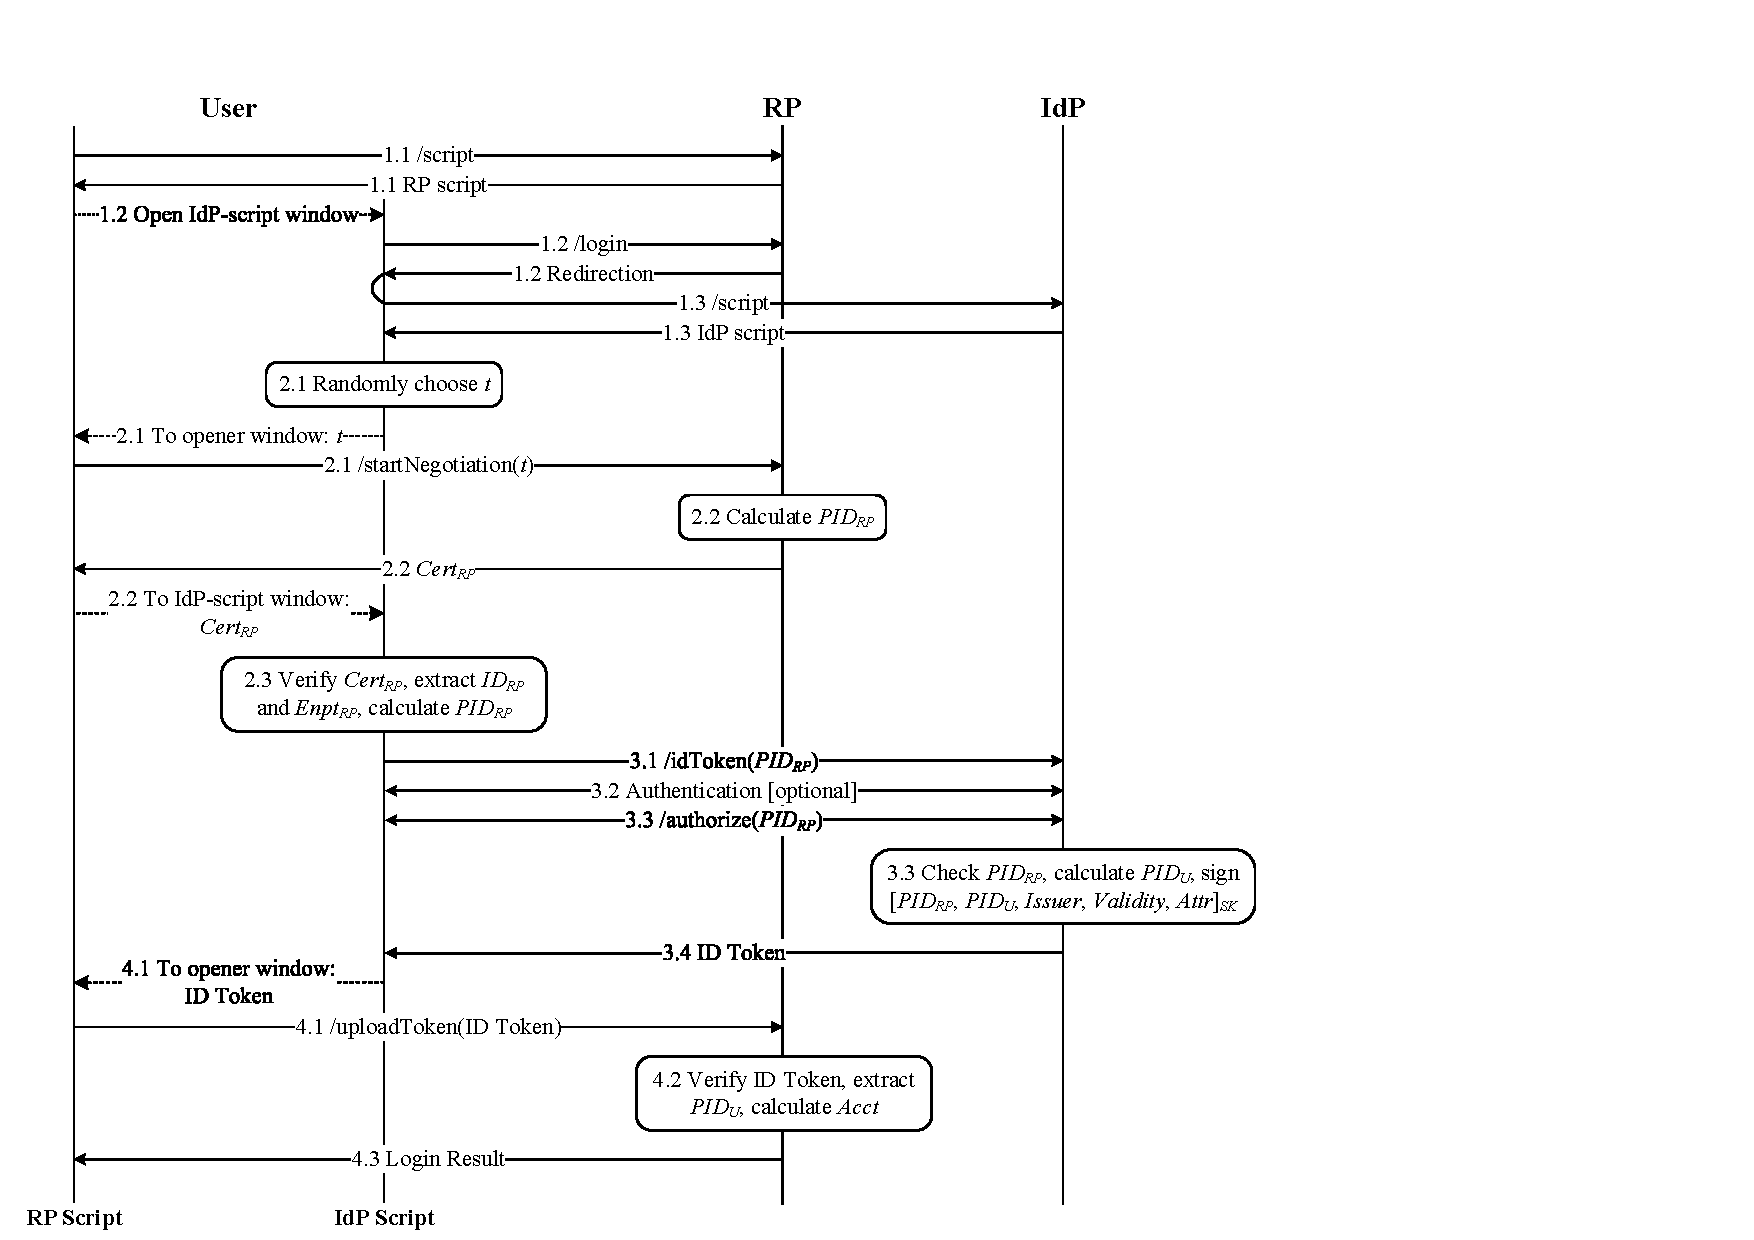
\includegraphics[height=0.82\textheight]{fig/process-js.pdf}
  \caption{The SSO login flow of UPPRESSO.}
  \label{fig:process}
\end{figure*}

\noindent \textbf{System Initialization.}
%In particular, the IdP %chooses $L$,
%generates a large prime $p$, and a prime factor $q$ of $p-1$
% and a generator $g$ of order $q$
%as the parameters of the discrete logarithm problem. % \cite{gallagher2013digital}.
The IdP generates a key pair ($SK$, $PK$) to sign/verify identity tokens and RP certificates.
%The lengths of %$p$, $q$ and
%($SK$, $PK$) should satisfy the required security strength.
Then, the IdP keeps $SK$ secret, while $PK$ is publicly known.
%The values of $p$, $q$, $g$ remain the same during the full lifecycle of an SSO system.
%While, the asymmetric key pair ($SK$, $PK$) will be updated when necessary. For example, when $SK$ is leaked, IdP must update ($SK$,$PK$).


\vspace{1mm}
\noindent\textbf{RP Initial Registration.} Each RP launches
    an initial registration operation once to finish configurations.
In particular, an RP registers itself at the IdP to obtain $ID_{RP}$
 and the corresponding RP certificate $Cert_{RP}$ as follows:
\begin{enumerate}
\vspace{-\topsep}\item
The RP sends a registration request to the IdP, including the RP endpoint to receive identity tokens,
    and other optional information.
\vspace{-\topsep}\item
The IdP generates a unique random number $r$, calculates $ID_{RP} = [r]G$,
    and assigns $ID_{RP}$ to this RP.
The IdP then signs $Cert_{RP} = [ID_{RP}, Enpt_{RP}, *]_{SK}$,
     where $[\cdot]_{SK}$ means a message signed using $SK$ and $*$ denotes supplementary information such as the RP's common name and Email,
     and returns $Cert_{RP}$ to the RP.
\vspace{-\topsep}\item
The RP verifies $Cert_{RP}$ using $PK$,
    and accepts $ID_{RP}$ and $Cert_{RP}$ if they are valid.
\vspace{-\topsep}\end{enumerate}
%\begin{itemize}
%\item The RP sends a registration request to the IdP, including the RP endpoint (e.g., URL) to receive identity tokens.
%\item The IdP generates the unique generator $ID_{RP}$,
%chooses a unique random number $r$ ($1 < r < q$), calculates $ID_{RP} = g^r \bmod p$,
%signs $[ID_{RP}, Endpoint_{RP}, *]$ using $SK$, where $*$ denotes the supplementary information such as the RP's common name, and returns $Cert_{RP} = [ID_{RP}, Endpoint_{RP}, *]_{SK}$ to the RP, where $[\cdot]_{SK}$ means the message is signed using $SK$.
%\item The RP verifies $Cert_{RP}$ using $PK$ and accepts $ID_{RP}$ and $Cert_{RP}$ if they are valid.
%\end{itemize}


%Note that $ID_{RP}$ is generated by the IdP but not chosen by the RP;
%otherwise, a malicious RP might choose $ID_{RP}$ which reduces the difficulty to solve the ECDLP
%    (i.e., it is possible for the RP to derive $ID_U$ from $Acct = [ID_U]{ID_{RP}}$
%        or at least some information about $ID_U$).
%%%%%%%%%% ��ΪE����ĵ㣬����ѭ��Ⱥ����n��������ʱ�����ԣ������γɹ�����
%%%%%%%%%% ����Ҫ���ע���

\vspace{1mm}
\noindent\textbf{User Registration.}
UPPRESSO adopts a similar user registration operation as the ones in other SSO systems.
Each user registers once at the IdP to set up a unique user identity $ID_U$ and the corresponding credential.
%$ID_U$ can be chosen by the user or the IdP, as long as it is unique for each user.

\vspace{1mm}
\noindent\textbf{SSO Login.} An SSO login instance is typically launched through a browser,
when a user requests to login an RP.

It consists of five steps, namely script downloading, RP identity transformation, $PID_{RP}$ registration, identity-token generation, and $Acct$ calculation, as shown in Figure \ref{fig:process}.
In this figure,
    the operations by the IdP are linked by a vertical line,
        so are the RP's operations.
Two vertical lines split the user's operations into two groups (i.e., in two browser windows),
    one of which is to communicate with the IdP,
                 and the other with the target RP.
Each solid horizontal line means some messages between the user and the IdP (or the RP),
            and each dotted line means a \verb+postMessage+ invocation between two scripts (or windows) within the browser.

%In this figure, vertical bars stand for entity in the UPPRESSO system.
%At the user side, the vertical bars represent the browser's windows which are the containers of IdP and RP scripts.
%After a window is opened, the script in this window may change.
%For example, a window is opened at Step 1.2, and the script in this window belongs to the RP.
%However, after the redirection at Step 1.3, it visits the IdP server and downloads the script,
% so that the script inside this window changes into the IdP script.
%The main difference is that,
% the IdP script is only trusted by IdP server and allowed to communicate with IdP server.
% So does the RP script.

%%%, which calls three identifier-transformation functions following the login flow as shown in Figure \ref{fig:process}.
%%%Once a user attempts to login an RP, the SSO login is initiated.
%%%We use the OIDC implicit protocol flow as an example, to demonstrate  how to integrate the three functions $\mathcal{F}_{ID_{U} \mapsto PID_{U}}$, $\mathcal{F}_{ID_{RP} \mapsto PID_{RP}}$ and $\mathcal{F}_{PID_{U} \mapsto Account}$ into the typical SSO systems.

\vspace{0.5mm}
\noindent 1. {\em Script Downloading.}
The browser downloads the scripts from the IdP and the visited RP.
\begin{itemize}
\vspace{-\topsep}\item[1.1]
When attempting to visit any protected resources at the RP,
    the user downloads the RP script.
\vspace{-\topsep}\item[1.2]
The RP script opens a window in the browser to visit the login path at the RP, which is then redirected to the IdP.
\vspace{-\topsep}\item[1.3]
The redirection to the IdP downloads the IdP script.
\vspace{-\topsep}\end{itemize}


\noindent{\em 2. RP Identity Transformation.}
The user and the RP negotiate $PID_{RP} = [t]{ID_{RP}}$.
\begin{itemize}
%\setlength{\itemsep}{0pt plus 1pt}
\vspace{-\topsep}\item[2.1] The IdP script in the browser chooses a random number $t$ ($1 < t <n$) and sends it to the RP script through \verb+postMessage+.
Then, the RP script sends $t$ to the RP.
\vspace{-\topsep}\item[2.2] On receiving $t$,
the RP verifies $1 < t < n$ and calculates $PID_{RP}$.
%To acknowledge the negotiation of $PID_{RP}$,
The RP replies with $Cert_{RP}$, which is then transmitted from the RP script to the IdP script.  % through \verb+postMessage+.
\vspace{-\topsep}\item[2.3] The IdP script verifies $Cert_{RP}$, extracts $ID_{RP}$ and $Enpt_{RP}$ from $Cert_{RP}$ and calculates $PID_{RP}=[t]{ID_{RP}}$.
It then creates a random endpoint $PEnpt_{U}$ for this login instance,
    to receive identity tokens from the IdP.
    % as the RP endpoint required by IdP.�����Ѿ��޸���Э�飬IdP����requireʲô
\vspace{-\topsep}
\end{itemize}

%It is important to ensure that the RP endpoint is not tampered with by the adversary. In other OIDC systems, the IdP obtains the RP endpoint from RP registration and verifies the endpoint in the identity-token request. However, the IdP in UPPRESSO sees only a one-time endpoint. So, we ask the user to verify the correctness of the RP endpoint using the RP certificate. %which is signed by the IdP.

\noindent{\em 3. ${PID_{RP}}$ Registration.}
The user registers the ephemeral $PID_{RP}$ at the IdP.
It is conducted by the IdP script in the user's browser. %Otherwise, the IdP can associate $PID_{RP}$ and $ID_{RP}$.
\begin{itemize}
%\setlength{\itemsep}{0pt plus 1pt}
\vspace{-\topsep}
\item[3.1] The IdP script sends the $PID_{RP}$ registration request $[PID_{RP}, PEnpt_U, H(t)]$ to the IdP,
    where $H()$ is a collision-free one-way hash function.
\vspace{-\topsep}
\item[3.2] The IdP checks the list of unexpired $PID_{RP}$
    to verify the received $PID_{RP}$ is a unique point on $\mathbb{E}$ among them.
Then, it signs the response $[PID_{RP}, H(t), Validity]_{SK}$, %denoted as $RegToken$, ����������
 where $Validity$ indicates when $PID_{RP}$ will expire (typically, in 3 to 5 minutes).
The IdP maintains the list of $PID_{RP}$ and deletes expired ones from it.
\vspace{-\topsep}
\item[3.3] The IdP script forwards the registration result to the RP through the RP script.
\vspace{-\topsep}
\item[3.4] The RP verifies the IdP's signature, and accepts the result
 only if $PID_{RP}$ and $H(t)$ match those in the negotiation and it does not expire.
\vspace{-\topsep}
\item[3.5] The RP constructs an identity-token request with $PID_{RP}$ and $Enpt_{RP}$,
    which is then forwarded to the IdP script through the RP script.
\vspace{-\topsep}
\end{itemize}
$H(t)$ is a nonce to distinguish different login instances,
 because there is a very small probability that
  an identical $PID_{RP}$ is calculated for two RPs from two different pairs of $ID_{RP}$ and $t$
   (i.e., $[t]ID_{RP_j} = [tr]G = [t'r']G = [t']ID_{RP_{j'}}$).
This nonce prevents one $PID_{RP}$ registration result (and the subsequent identity token)
     from being accepted by multiple RPs.

\noindent{\em 4. Identity-Token Generation.}
The IdP calculates $PID_U = [ID_U]{PID_{RP}}$ and signs the identity token. % The processes are as follows.
\begin{itemize}
\vspace{-\topsep}
\item[4.1]
The IdP script checks that $PID_{RP}$ is the one registered in Step 3.1
            and $Enpt_{RP}$ matches the one in $Cert_{RP}$.
Then, the IdP script replaces $Enpt_{RP}$ with $PEnpt_{U}$ in the identity-token request
     and sends this modified request to the IdP.
\vspace{-\topsep}
\item[4.2] On receiving an identity-token request,
    the IdP authenticates the user if he has not been authenticated yet.
\vspace{-\topsep}
\item [4.3] 
After obtaining the user's authorization to enclose the requested attributes,
the IdP checks whether the received pair of $PID_{RP}$ and $PEnpt_U$ is in the list of unexpired $PID_{RP}$ or not,
    and calculates $PID_U = [ID_U]{PID_{RP}}$ for the authenticated user.
The IdP then signs an identity token $[PID_{RP}, PID_U, Iss, Validity, Attr]_{SK}$,
 where $Iss$ is the IdP's identity, $Validity$ is the validity period, and $Attr$ contains the requested attributes.
\vspace{-\topsep}
\item[4.4] The IdP sends the identity token to $PEnpt_{U}$.
\vspace{-\topsep}
\end{itemize}

\noindent{\em 5. $Acct$ Calculation.}
The RP verifies the identity token and allows the user to login.
\begin{itemize}
%\setlength{\itemsep}{0pt plus 1pt}
\vspace{-\topsep}
\item [5.1]
The IdP script forwards this token to the RP script,
    which then sends it to the RP through $Enpt_{RP}$.
\vspace{-\topsep}\item[5.2] The RP verifies the identity token, including the IdP's signature and its validity period.
It also verifies $PID_{RP}$ in the token is consistent with the one negotiated in the previous step.
Then, the RP extracts $PID_U$, calculates $Acct = [t^{-1}]{PID_U}$.
\vspace{-\topsep}
\item [5.3] The RP returns the login result, and allows the user to login as $Acct$.
\vspace{-\topsep}
\end{itemize}


If any verification or check fails in any step,
 the flow will be halted immediately.
For example, the user halts
    if $Cert_{RP}$ is invalid or
    $PID_{RP}$ in the identity-token request is inconsistent with the negotiated one.
The IdP rejects the identity-token request, if the pair of $PID_{RP}$ and $Endpoint_U$ is not in the unexpired list.
Or the RP rejects the login request,
    if $PID_{RP}$ in the token does not match the negotiated one.


\begin{comment}
\subsection{SSO Login Flow of UPPRESSO}
\label{sebsec:loginprocess}

We illustrate the steps of the SSO login protocol of UPPRESSO in Figure \ref{fig:process}, %the SSO login sub-protocol provides the secure SSO service and prevents both the IdP-based login tracing and RP-based identity linkage.
 % prevents the curious IdP from obtaining the RP's identifying information during the interchanges,
%  and avoids the adversary to break the security and user's privacy.
and describe the detailed processes as follows.

\begin{figure*}
  \centering
  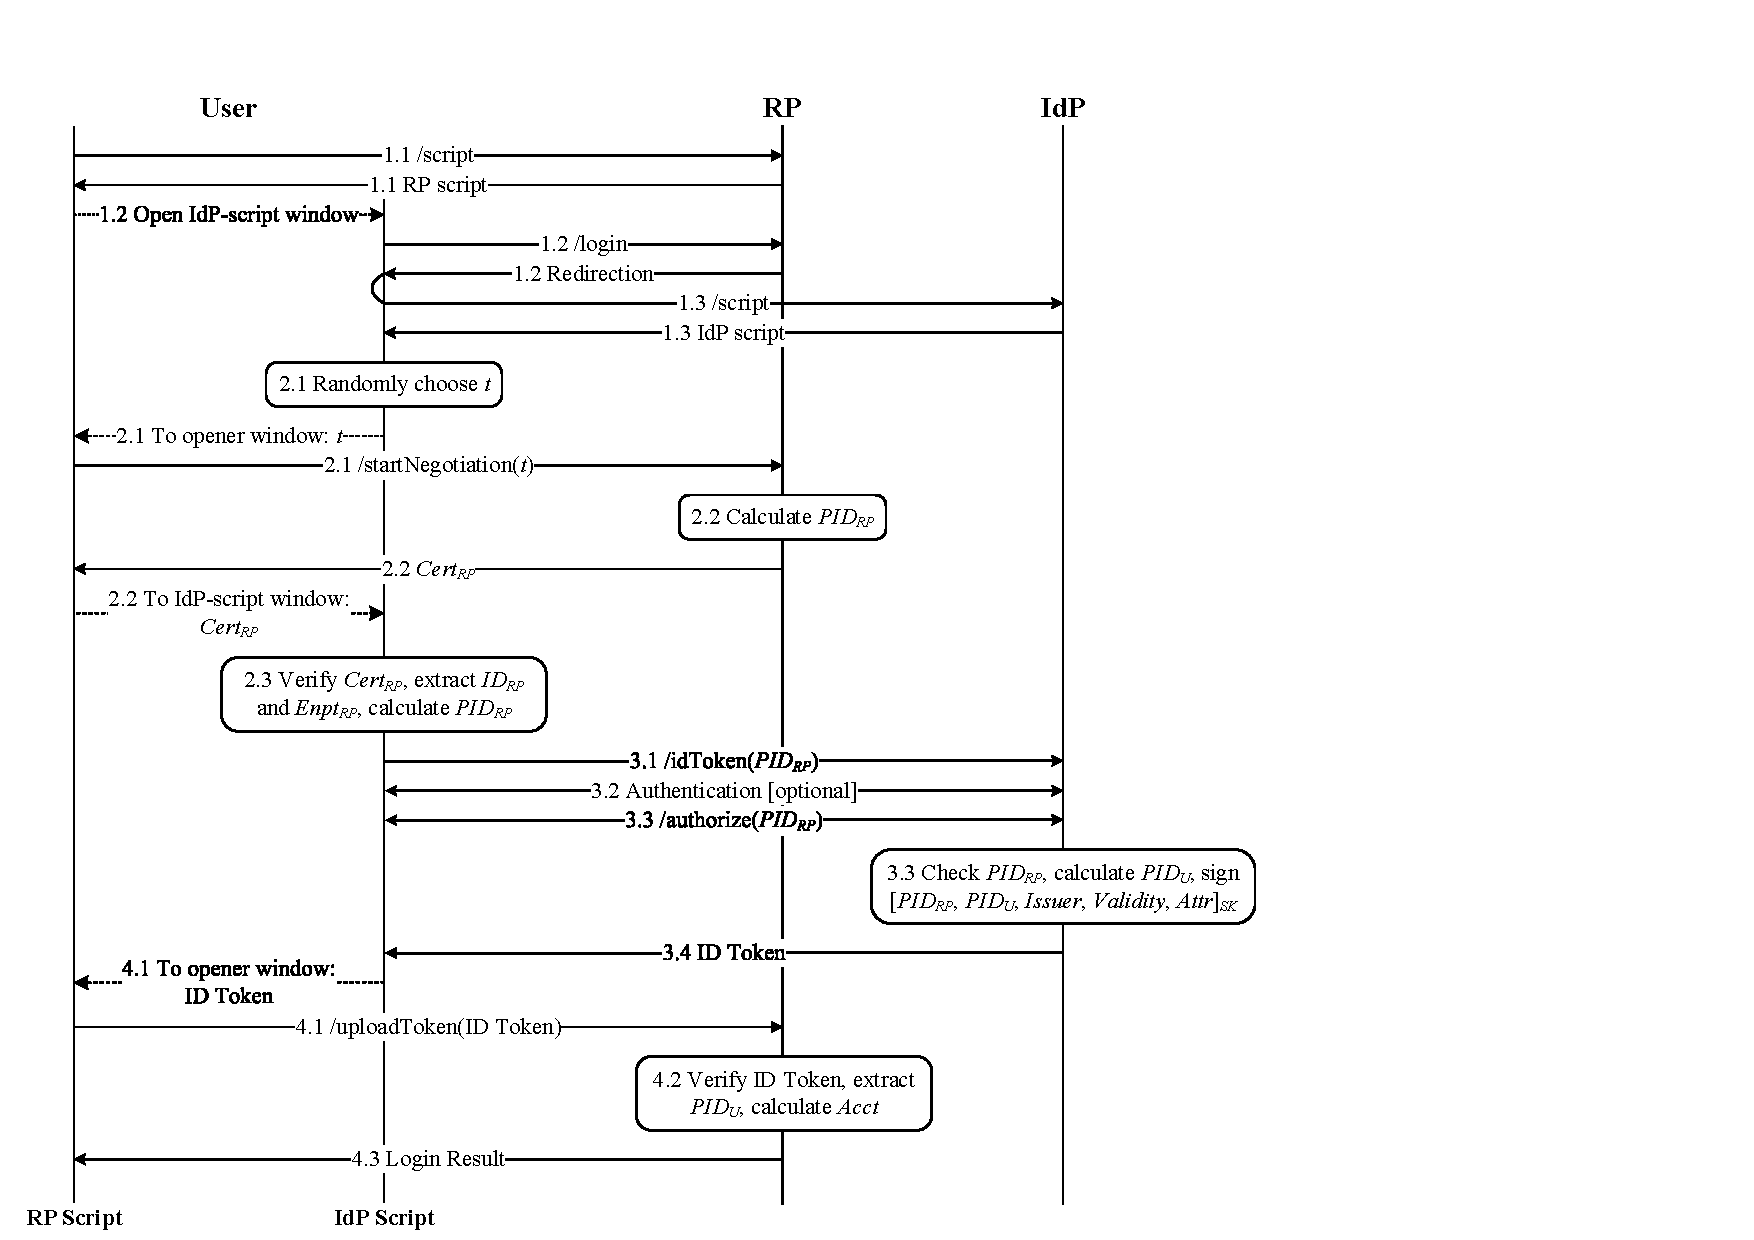
\includegraphics[width=0.68\linewidth]{fig/process-js.pdf}
  \caption{The flow of a user login in UPPRESSO.}
  \label{fig:process}
\end{figure*}

\vspace{1mm}\noindent\textbf{Scripts Downloading.}
At the beginning, the user downloads the scripts from RP and IdP as follows:\\

\begin{itemize}
\item[1.1] The user  visits the RP's script site and downloads the script.
\item[1.2] The script opens a new window in the browser visiting the login path at RP.
\item[1.3] The visit to RP's login path is redirected to IdP's script.
\item[1.4] The new window visits  the IdP's script site and downloads the script.
\end{itemize}

\vspace{1mm}\noindent\textbf{RP Identifier Transformation.}
In this step, the user and the RP cooperate to generate $PID_{RP}$ as follows:
\begin{itemize}
\item[2.1] The IdP script chooses a random number $N_U$ ($1 < N_U <q$) and sends it to RP script through postMessage, then RP script sends $N_U$ to RP.
\item[2.2] The RP  verifies $N_{U} \neq 0 \bmod q$, calculates $PID_{RP}$ with $N_U$, derives the trapdoor $T={(N_U N_{RP})}^{-1} \bmod q$; and  acknowledges the negotiation by responding with $Cert_{RP}$. The $Cert_{RP}$ is transmitted from RP script to IdP script through postMessage.
\item[2.3] The IdP script verifies $Cert_{RP}$, extracts $ID_{RP}$ from the valid $Cert_{RP}$,  calculate $PID_{RP}={ID_{RP}}^{N_{U}} \bmod p$, creates a one-time endpoint to hide the RP's endpoint from the IdP and calculates $Nonce=Hash(N_U)$.


 % \item [1.1] The user sends a login request to trigger the negotiation of $PID_{RP}$.
%  \item [1.2] The RP chooses a random number $N_{RP}$ ($1 < N_{RP} <q$), calculates $Y_{RP}={ID_{RP}}^{N_{RP}} \bmod p$, % (Step 2.1.1);
%   and sends $Y_{RP}$ with $Cert_{RP}$  to the user. % (Step 2.1.2).
%  \item [1.3] The user verifies $Cert_{RP}$, extracts $ID_{RP}$ from the valid $Cert_{RP}$, chooses a random number $N_U$ ($1 < N_U <q$) to calculate $PID_{RP}={Y_{RP}}^{N_{U}} \bmod p$, and sends $N_U$ %with $PID_{RP}$
%       to the RP.
%  \item [1.4] The RP verifies $N_{U} \neq 0 \bmod q$, calculates $PID_{RP}$ with $N_U$ and $Y_{RP}$, %checks its consistency with the received one,
 %  derives the trapdoor $T={(N_U N_{RP})}^{-1} \bmod q$; and
%   acknowledges the negotiation by responding with $N_{RP}$.
 % \item [1.5] The user verifies that $N_{RP} \neq 0 \bmod q$ and $Y_{RP} = {ID_{RP}}^{N_{RP}} \bmod p$.
   %sends the calculated $PID_{RP}$ to the user (Step 2.1.6).
%  \item The user checks the consistency of the received $PID_{RP}$ with the stored one.
\end{itemize}

The user halts the negotiation, if  $Cert_{RP}$ is invalid.
%The verification of $Y_{RP}$ and $N_{RP}$ ensures the order of $Y_{RP}$ (and also $PID_{RP}$) is $q$,
  %  and prevents a malicious RP from choosing an arbitrary $Y_{RP}$ (then $PID_{RP}$) of order less than $q$,
    %    which makes it less difficult for the RP to derive $ID_U$ from $PID_U$.
 %or the received $PID_{RP}$ is different from the stored one. The RP also halts the process if the $PID_{RP}$ sent by the user is inconsistent with the calculated one.
%The user verifies that  \textcolor[rgb]{1.00,0.00,0.00}{$PID_{RP}$ is in the cyclic  group defined by $g$},
%$PID_{RP} \neq g^0 \bmod p$;
%    if $PID_{RP} = g^0 \bmod p$, $PID_U = {g}^{0*ID_U}$ is constant for all users.
%This case appears only if  $N_U = 0 \bmod q$ or $N_{RP} = 0 \bmod q$.

\vspace{1mm}\noindent\textbf{$\mathbf{PID_{RP}}$ Registration.}
The user registers $PID_{RP}$ at the IdP.
\begin{itemize}

\item[3.1] The IdP script sends the ${PID_{RP}}$ registration request $[PID_{RP}, Hash( N_U), Endpoint_U]$ to the IdP.
\item[3.2] The IdP verifies that $PID_{RP}$ is unique among unexpired $PID_{RP}$s,
    and then signs the response $[PID_{RP}, Hash( N_U), Validity]_{SK}$,
        where $Validity$ is the validity period.
\item[3.3] The IdP script forwards the registration result to the RP through RP script.
\item[3.4] The RP verifies the IdP's signature, and accepts it only if $PID_{RP}$ and $Hash(N_U)$ match those in the negotiation and it is in the validity period.


 % \item [2.1] The user creates a one-time endpoint to hide the RP's endpoint from the IdP, and sends the ${PID_{RP}}$ registration request $[PID_{RP}, Hash(N_{RP}, N_U), Endpoint_U]$ to the IdP.
  %\item [2.2] The IdP authenticates the user if she has not been authenticated yet.
  %The IdP verifies that $PID_{RP}$ is unique among unexpired $PID_{RP}$s,
   % and then signs the response $[PID_{RP}, Hash(N_{RP}, N_U), Validity]_{SK}$,
      %  where $Validity$ is the validity period.
%The IdP returns the signed response to the user.
 % \item [2.3] The user forwards the registration result to the RP.
  %\item [2.4] The RP verifies the IdP's signature, and accepts it only if $PID_{RP}$ and $Hash(N_{RP}, N_U)$ match those in the negotiation and it is in the validity period.
\end{itemize}

%If $RegRes$ is $OK$, the RP identifier refreshing completes. Otherwise, the user and RP will renegotiate the $PID_{RP}$.
$Hash(N_U)$ is attached as the nonce to avoid the registration result is accepted by two or more RPs,
 which have different $ID_{RP}$s but generate a same $PID_{RP}$.  % with a negligible possibility.
The IdP ensures $PID_{RP}$ is unique among unexpired ones;
 otherwise, one identity token for one $PID_{RP}$ might be accepted by other RPs.
%The RP checks if Hash($N_{RP}$, $N_U$) matches,
%    to ensure this is signed for it (not for other RPs).
More details are analyzed in Section \ref{sec:analysis}.

\vspace{1mm}\noindent\textbf{ID Token Generation.}
In this step, the user login continues and the IdP signs the identity token. % The processes are as follows.
\begin{itemize}
\item[4.1] The RP uses $PID_{RP}$ and $Endpoint_{RP}$ to construct an identity-token request for a set of user's attributes, and the request is forwarded to IdP script through RP script.
\item[4.2] The IdP authenticates the user if she has not been authenticated yet.
 \item[4.3] The user first confirms the scope of the requested attributes. IdP script verifies the $PID_{RP}$ with the negotiated one and $Endpoint_{RP} \in Cert_{RP}$, replaces the endpoint with the registered one-time $Endpoint_U$ and then sends the modified identity-token request to the IdP.
 \item [4.4] The IdP verifies whether $PID_{RP}$ and $Endpoint_U$ have been registered and unexpired, and
   calculates $PID_U = {PID_{RP}}^{ID_U} \bmod p$ for the authenticated user.
\item[4.5] The IdP constructs and signs the identity token $[PID_{RP}, PID_U, Iss, ValTime, Attr]_{SK}$, where $Iss$ is the identifier of the IdP,  $ValTime$ is the validity period, $Attr$ contains the requested attributes.
\item[4.6]Then, the IdP sends the identity token to the one-time endpoint at the user. The IdP script forwards the identity token to RP script with the origin $Endpoint_{RP}$ and RP script sends it to the server.

%  \item [3.1] The RP uses $PID_{RP}$ and $Endpoint_{RP}$ to construct an identity-token request for a set of user's attributes.  %, which is the same as the one in  OIDC.

 %\item [3.2] The user first confirms the scope of the requested attributes and verifies $PID_{RP}$ with the negotiated one. The user replaces the endpoint with the registered one-time $Endpoint_U$, and sends the modified identity-token request to the IdP.
%  \item [3.3] The IdP verifies whether $PID_{RP}$ and $Endpoint_U$ have been registered and unexpired, and
%   calculates $PID_U = {PID_{RP}}^{ID_U} \bmod p$ for the authenticated user.
%\item [3.4] The IdP constructs and signs the identity token $[PID_{RP}, PID_U, Iss, ValTime, Attr]_{SK}$, where $Iss$ is the identifier of the IdP,  $ValTime$ is the validity period, $Attr$ contains the requested attributes. Then, the IdP sends the identity token to the one-time endpoint at the user.
%  \item [3.5] The user extracts the RP endpoint in $Cert_{RP}$,
  % and forwards the identity token to the RP through this endpoint.
\end{itemize}

The user halts the process if $PID_{RP}$ in the identity-token request is inconsistent with  the negotiated one.
The IdP rejects the identity-token request, if the pair of $PID_{RP}$ and $Endpoint_U$ has not been registered.


\vspace{1mm}\noindent\textbf{$\mathbf{Account}$ calculation.}
Finally, RP derives the user's  $Account$ and completes the user login as follows.
\begin{itemize}
\item[5.1]
The RP verifies the identity token, including the signature, validity period, and the consistency between $PID_{RP}$ and the negotiated one. If any fails, the RP rejects this login.
\item [5.2] The RP extracts $PID_U$, calculates $Accout = {PID_U}^T \bmod p$, and allows the user to login.
\end{itemize}
%
%\begin{figure}[t]
%  \centering
%  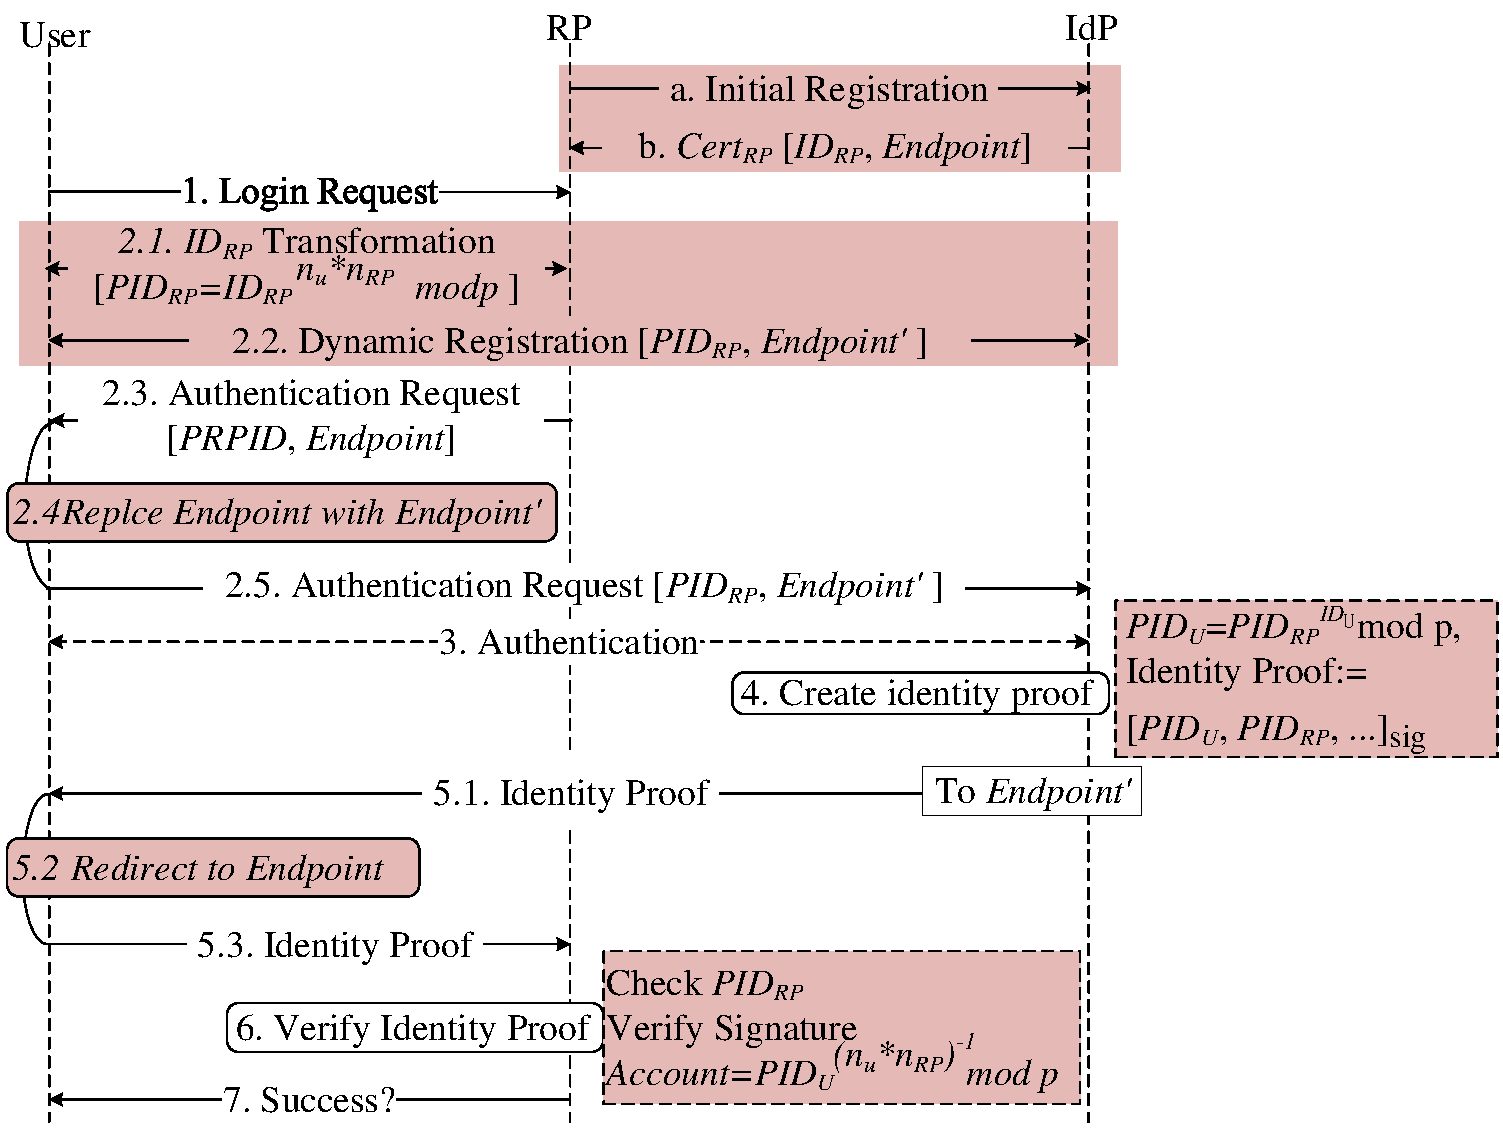
\includegraphics[width=\linewidth]{fig/overview1.pdf}
%  \caption{UPPRESSO compatibility with OIDC.}
%  \label{fig:UPPRESSO}
%\end{figure}
%

\end{comment}



\begin{comment}
\vspace{1mm}
\begin{strip}
\centering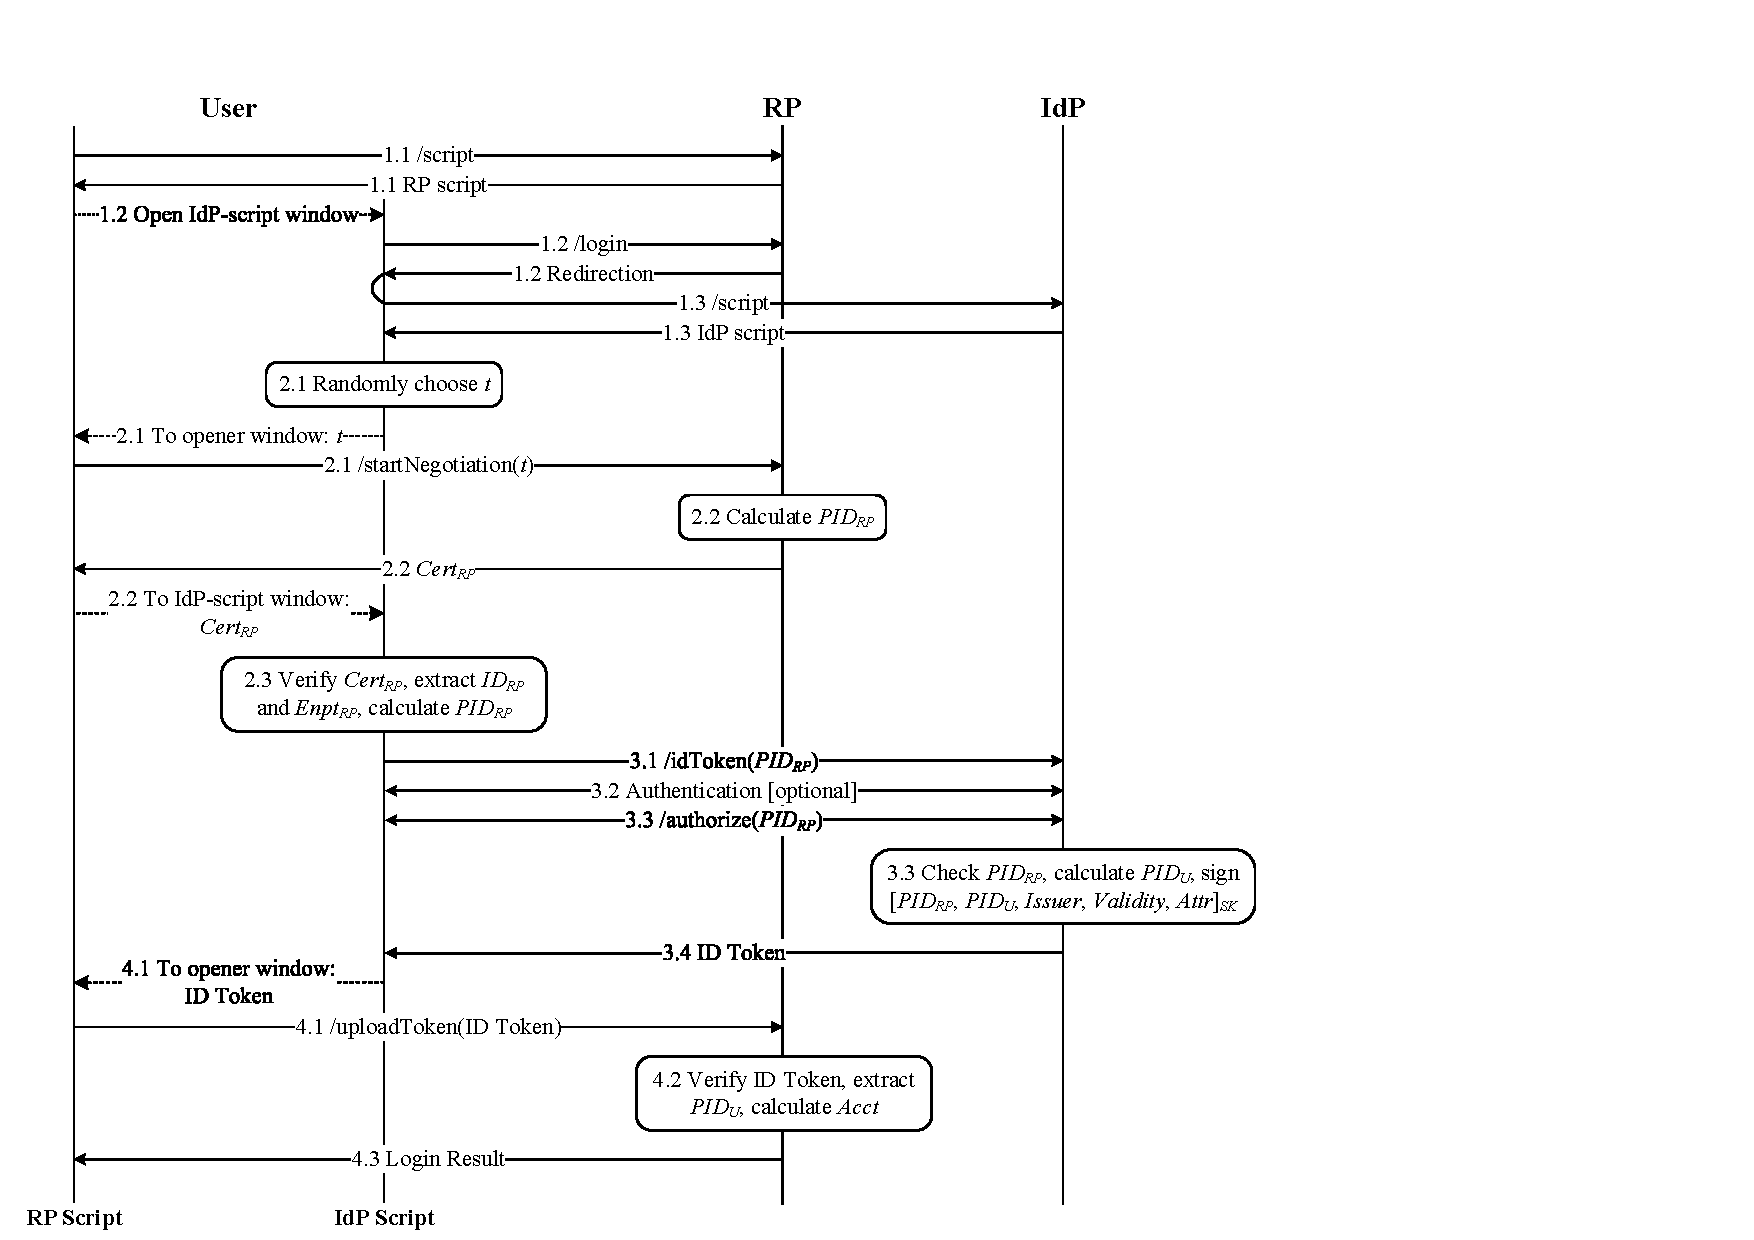
\includegraphics[width=0.5\textwidth]{fig/process-js.pdf}
\captionof{figure}{The flow of a user login in UPPRESSO.}
\label{fig:process}
\vspace{-5mm}
\end{strip}
\end{comment}

\subsection{Compatibility with OIDC}
\label{subsec:compatible}
%We explain the compatibility with OIDC,
%    and this compatibility helps us to analyze, implement and deploy UPPRESSO.
% ��仰ǰ���Ѿ�˵����


Among the five steps of the SSO login flow in UPPRESSO,
    the script downloading prepares the user agent.
The user agent deals with the communications between the IdP and the RP,
    which are redirected by browsers in OIDC.
In UPPRESSO,
    when sending the identity-token request,
        the script replaces $Enpt_{RP}$ with $PEnpt_{U}$,
    and when forwarding the identity token,
            the script forwards this token to $Enpt_{RP}$ maintained by the script itself.

In the step of RP identity transformation, most operations are conducted by the user agent while the RP only receives $t$ to calculate $PID_{RP}$ and sends $Cert_{RP}$.
The operations in the $PID_{RP}$ registration are almost identical to those in the RP Dynamic Registration of OIDC \cite{DynamicRegistration},
    except that
    the IdP of OIDC assigns the RP's identity  while this (pseudo-)identity in UPPRESSO is generated by the registered entity.

The operations in the steps of identity-token generation and $Acct$ calculation,
    are actually identical to those in the implicit SSO login flow of OIDC \cite{OpenIDConnect},
    while (\emph{a}) the calculation of $PID_U$ is viewed as a method to generate PPIDs by the IdP
        and (\emph{b}) the calculation of $Acct$ is viewed as a mapping from the user identity in tokens
                    to the local account at the RP.


%It follows a similar logic flow as OIDC in SSO login and only requires small modifications to perform identifier transformation.
%Here, we explain the modification in each of the five steps of its SSO login flow to show that UPPRESSO is compatible with OIDC, which indicates UPPRESSO can be easily integrated with other commonly used SSO systems.
%Among the five steps,
% the {\em scripts downloading} and {\em RP identifier transformation} steps are newly introduced by UPPRESSO.
%The browser is required to download two scripts from the IdP and RP and most of the designed operations in these two steps are performed by the scripts in the browser.
%So, we require minimal modifications to the IdP and RPs providing new network interfaces (i.e., the new URLs for downloading resources).
%The other three steps adopt a similar communication pattern as OIDC.
%In particular, the {\em $PID_{RP}$ registration} step can be viewed as a variant of the RP dynamic registration flow of OIDC \cite{DynamicRegistration}, which allows an entity to register its identity and endpoint at the IdP.

%UPPRESSO can also support the authorization code flow of OIDC with small modifications (to be discussed in Section \ref{sec:discussion}).


%Different from OIDC in which only RPs can call a dynamic registration, UPPRESSO allows any authenticated user to launch this process and register an RP identifier with the IdP.
%The {\em identity token generation} and {\em $Account$ calculation} steps adopt the same steps and functions as the implicit protocol flow of OIDC, while using a few different parameters. First, in identity token generation, $PID_U$ transformed from $ID_U$ is used to replace $ID_U$, which is directly supported by OIDC, similar as in the PPID approaches that also convert $ID_U$ into $PID_U$. The calculation of $Account$ from $PID_U$
%can be viewed as a customized step by the RP to derive its user account after the implicit protocol flow of OIDC ends.

%So,the identity token generation and $Account$ calculation steps of UPPRESSO can be viewed as a particular but compatible implementation of the implicit protocol flow of OIDC. It is worth noting that the identity token generation and $Account$ calculation steps of
%As shown in Figure \ref{fig:process}, in UPPRESSO, the SSO protocol for identity token is the same as in OIDC; the formats of identity token and corresponding request are the same as in OIDC; the correctness checks on the identity-token request at the IdP (i.e., consistency of RP' identifier and endpoint with the registered one) are the same as in OIDC; the correctness checks on the identity token (i.e., consistency of RP' identifier with the one in the request, integrity, validity time, freshness, and etc.) at the RP are the same as in OIDC.
%The above modifications could be completed automatically for each login, without affecting other communication pattern.

%����Ϊ����Step 2.3��7����ϸ����.
%That is, the RP construct a request for identity token (Step 2.3); the user redirects this request to the IdP (Step 2.5); the IdP generates the identity token (Step 4), and sends it to the user (Step 5.1) who redirects it to the RP (Step 5.3); and finally the RP verifies the identity token (Step 6).

%However, UPPRESSO achieves privacy preservation by integrating  $\mathcal{F}_{ID_{U} \mapsto PID_{U}}$, $\mathcal{F}_{ID_{RP} \mapsto PID_{RP}}$ and $\mathcal{F}_{PID_{U} \mapsto Account}$, and  introduces the following modifications on OIDC.

%\begin{enumerate}
%  \item The identity token is bound with $PID_{RP}$ instead of $ID_{RP}$, which introduces the RP identifier transforming (Steps 1.2-1.5)  and $PID_{RP}$ registration (Steps 2.1-2.4).
%  \item The identity token is designated to one-time endpoint instead of RP's identifying endpoint, which requires the user to register the one-time endpoint in Step 2.1 and replace it with the original endpoint in Step 3.2.
%  \item IdP generates $PID_U$ based on ($PID_{RP}$, $ID_U$) instead of ($ID_{RP}$, $ID_U$).
%  \item The RP calculates $Account$ from the changing $PID_U$ instead of an unchanged one.
%\end{enumerate}

%����modification���ʵ�ֵģ�������
%to add: PID_{RP} transforming �� RP identifer refreshing��user��RP��ҳ���Լ�����ˡ� �����ֳɵ����ݸ�ʽ
%one-time endpoint ��endpoint
%The user automatically invokes the JavaScript functions to complete RP identifier transforming, one-time endpoint generating/replacing and $PID_{RP}$ registration for each login.
%While, the RP and IdP provide the corresponding web service to complete the processing automatically.

%The protocol of RP identifier transformation is based Diffie-Hellman key exchange \cite{DiffieH76}, while $N_U$ is provided to RP for computing the trapdoor and $N_{RP}$ is provided to the user for verifying the correctness of $Y_{RP}$.

\begin{comment}
\vspace{1mm}\noindent \textbf{Consistency with OIDC.}
As shown in Figure \ref{fig:UPPRESSO}, the architecture of UPPRESSO is the same as the one in OIDC. UPPRESSO does not introduce any new entity, but only integrates the three function $\mathcal{F}_{ID_{U} \mapsto PID_{U}}$, $\mathcal{F}_{ID_{RP} \mapsto PID_{RP}}$ and $\mathcal{F}_{PID_{U} \mapsto Account}$ into the processes at the IdP, RP, and user.

The formats of the  identity token and corresponding request, and the verification of the identity token,  are almost same in OIDC and UPPRESSO.
The only difference is that $ID_{RP}$ and endpoint are replaced with the privacy-preserving versions, i.e., $PID_{RP}$ and one-time endpoint, in UPPRESSO.
As $PID_{RP}$ is also unique and corresponds exactly to $ID_{RP}$, and one-time endpoint corresponds to the RP's endpoint correctly,
 the binding, integrity and confidentiality of identity token will also be ensured in UPPRESSO, and there is no degradation on the security of OIDC.

\vspace{1mm}\noindent \textbf{Minimal modification to OIDC.}
UPPRESSO only requires small modification on OIDC to integrate $\mathcal{F}_{ID_{U} \mapsto PID_{U}}$, $\mathcal{F}_{ID_{RP} \mapsto PID_{RP}}$ and $\mathcal{F}_{PID_{U} \mapsto Account}$.
For $\mathcal{F}_{ID_{U} \mapsto PID_{U}}$ and $\mathcal{F}_{PID_{U} \mapsto Account}$, we directly use them to replace original functions for $PPID$ at the IdP and the $Account$ at the RP.
For $\mathcal{F}_{ID_{RP} \mapsto PID_{RP}}$, we inject a negotiation process and a dynamic registration for each SSO login,
 where the negotiation process between the user and RP generates a $PID_{RP}$,
  while the dynamic registration is used to check the uniqueness of $PID_{RP}$.
In UPPRESSO, the dynamic registration is slightly modified as follows: an RP identifer ($PID_{RP}$)  is added in the request, and a signature ($Sig_{Res}$)  is included in the response for its verification at the RP.
\end{comment}

\section{Security Analysis}
\label{sec:formal}
%Our formal analysis of UPPRESSO is based on the Dolev-Yao style web model presented in ~\cite{SPRESSO}. However, in this paper we simplify the model, in particularly we assumed that DNS servers are always honest and the DNS requests and responses are always handled securely so that they are not considered in our model.  Moreover, we assume that HTTPs protocol is hundred-percent adopted and securely implemented, such that the web communications are secure and we will not focus on the encryption and decryption of these communications.

We formally analyze the security and privacy properties of UPPRESSO based on the Dolev-Yao style web model~\cite{SPRESSO}, which has been widely used in the formal analysis of SSO protocols such as OAuth 2.0~\cite{FettKS16} and OIDC~\cite{FettKS17}. For brevity, we focus on the modifications introduced by UPPRESSO in this paper and neglect the proofs for the security of DNS and HTTPS requests. We refer interested readers to~\cite{SPRESSO} for details.

\subsection{The Web Model}
\label{subsec:webmodel}
The Dolev-Yao model abstracts the entities in a system, such as browsers and web servers, as {\em atomic processes}, which communicate with each other through the {\em events}. \cite{SPRESSO} also defines {\em scripting processes} to model client-side scripting such as JavaScript, so a web system consists of a set of atomic and scripting processes. The state of a system, called a {\em configuration}, consists of the current states of all atomic processes and all the events that can be accepted by these processes. We list the definitions of these notations as below~\cite{SPRESSO}.

%\vspace{1mm}
\noindent{\em Messages} are defined as formal terms without variables (i.e., ground terms) over a {\em signature}. %Terms are defined as names, variables and function symbols. A function symbol with arity 0 (with no arguments) is a constant symbol.
The signature $\Sigma$ consists of a finite set of function symbols (with arity). For messages in this mode, the signature $\Sigma$ contains constants such as ASCII strings and nonce, sequence symbols such as n-ary sequences $\langle \rangle$, $\langle . \rangle$, $\langle . ,. \rangle$, and function symbols that model cryptographic primitives such as $\mathtt{encrypt}, \mathtt{decrypt}$ and digital signatures. For example, an HTTP request can be modeled as a ground term containing a type (e.g., $\mathtt{HTTPReq}$), a nonce, a method (e.g., $\mathtt{GET}$ or $\mathtt{POST}$), a domain, a path, URL parameters, request headers and a message body, over the $\Sigma$ in the sequence symbol format. So,
an HTTP GET request for the domain {\sf exa.com/path?para=1} with empty header and body can be represented as: $m:=\langle\mathtt{HTTPReq},n,\mathtt{GET},exa.com,/path,\langle \langle para, 1\rangle \rangle ,\langle \rangle,\langle \rangle \rangle$.

\noindent{\em Events} are the basic communication elements in the model. An event is of the form $\langle a, f, m \rangle$, where $a$ and $f$ represent the addresses of the sender and receiver respectively, and $m$ is the message to be transmitted.

\noindent{\em Atomic Processes.} An {\em atomic Dolev-Yao (DY) process} is a tuple $p=$ $(I^p, Z^p, R^p,s_0^p )$, where $I^p$ is the set of addresses that the process listens to, $Z^p$ is the set of states (i.e., terms) that describes the process, $s_0^p$ is an initial state, and $R^p$ is the mapping from an input state $s \in Z^p$ and an event $e$ to a new state $s'$ and an event $e'$. %It is worth noting that for one process in a state, only a finite set of events can be accepted by the process as the state and event are defined as the input of $R^p$.
Each atomic process also contains a set of nonces that it may use.

\noindent{\em Scripting Processes} represent client-side scripts loaded by the browser to provide server-defined functions to the browser. However, a scripting process must rely on an atomic process, such as the browser, and provide the relation $R$ called by this atomic process.

\noindent{\em Equational theory} is defined as usual in Dolev-Yao models, which uses the symbol $\equiv$ to represent the congruence relation on terms. For example, $dec(enc(m, k), k)$ $\equiv$ $m$, where $k$ is a symmetric key.

\noindent {\em Static equivalence.} As defined in~\cite{SPRESSO}, two messages $t_1$ and $t_2$ are statically equivalent, denoted as $t_1 \approx t_2$, if and only if, for all terms such as $M(x)$ and $N(x)$ which only contain one variable $x$ without nonce, it is true that $M(t_1)$ $\equiv$ $N(t_1)$ \textbf{iff} $M(t_2)$ $\equiv$ $N(t_2)$. For instance, for messages $m$ and $m'$, and a symmetric key $k$, $enc(m, k)$ $\approx$ $enc(m', k)$ is always true to the attacker who does not know $k$.

Using static equivalence, we define equivalence of $modpow$ function as below. We also define equivalence of HTTP requests and events. Please find the details of the definitions in the Appendix.
\begin{definition}
For a large prime $p$ (2048-bit length) and $p-1$'s prime factor $q$ (256-bit length), there are two constants $g_1$, $g_2$ as the generators of $p$ and the constants $n_1$, $n_2$ ($n_1$, $n_2$ $<$ $q$). We define the function symbol $modpow(a, b, p)$ $=$ $a^b \mod p$, there are $modpow(g_1, n_1, p)$ $\approx$ $modpow(g_2, n_2, p)$ and  $modpow(g_1, n_1, p)$ $\approx$ $modpow(g_1, n_2, p)$  always true due to the discrete logarithm problem as the $n_1$ and $n_2$ are unknown.
\label{def:powequ}
\end{definition}
\begin{comment}
\begin{definition}
\noindent\textbf{Equivalence of HTTP requests}. There are messages $m_1$ and $m_2$, we say that $m_1$ $\approx$ $m_2$ \textbf{iff} the following conditions are met,
\vspace{-\topsep}
\begin{itemize}
\setlength{\itemsep}{0pt plus 1pt}
\item If $m_1$ and $m_2$ are HTTPs requests, they are  equivalent to the observers besides of the receiver.
\item If  $m_1$ and $m_2$ are HTTPs requests, they are equivalent for the receiver \textbf{iff} the value of the Host,Path,Origin and Referer headers in both requests are same, as well as the value of the Parameters and Body are statically equivalent.
\item If  $m_1$ and $m_2$ are HTTP requests, they are equivalent to all the observers as the equivalent HTTPS requests to receivers.
\end{itemize}
\setlength{\itemsep}{0pt plus 1pt}
\label{def:httpequ}
\end{definition}
\begin{definition}
\noindent\textbf{Equivalence of events}.
There are events $e_1$ := $\langle a_1, f_1, m_1 \rangle$ and $e_2$ := $\langle a_2, f_2, m_2 \rangle$, we say that $e_1$ $\approx$ $e_2$ \textbf{iff}
\vspace{-\topsep}
\begin{itemize}
\item $a_1$ $\equiv$ $a_2$ or $a_1$ and $a_2$ belong to random addresses.
\item $f_1$ $\equiv$ $f_2$ or $f_1$ and $f_2$ belong to random addresses.
\item $m_1$ and $m_2$ are equivalent.
\end{itemize}
\label{def:eventequ}
\end{definition}
\vspace{-\topsep}
\end{comment}

\noindent {\bf Web system.} We can represent the web infrastructure as a web system of form ($\mathcal{W}$, $\mathcal{S}$, $\mathtt{script}$, $E^0$), where $\mathcal{W}$ is the set of atomic processes containing both honest and malicious processes, $\mathcal{S}$ is the set of scripting processes including honest and malicious scripts, $\mathtt{script}$ is the set of concrete script codes related to specific scripting processes in $\mathcal{S}$, and $E^0$ is the set of events acceptable to the processes in $\mathcal{W}$.

\noindent A {\em configuration} of this web system is a tuple ($S, E, N$), where $S$ is the current states of all processes in $\mathcal{W}$, $E$ is the set of events that the processes accept, and $N$ is a global sequence of nonces that have not been used by the processes yet.

\noindent A {\em run step} is the system migrating from configurations ($S, E, N$) to ($S', E', N'$) by processing an event $e \in E$.

\subsection{The Formal Model of UPPRESSO}
Accordingly, we model UPPRESSO as a web system, which is defined as $\mathcal{UWS} = (\mathcal{W}, \mathcal{S}, \mathtt{script}, E^0)$. $\mathcal{W}$ is a finite set of atomic processes in UPPRESSO, which contains an IdP server process, a finite set of web servers for the honest RPs, a finite set of honest browsers, and a finite set of attacker processes. Here, we consider all the RP processes and browser processes are honest, and model an RP or a browser controlled by an adversary as an atomic attacker process.
%We assume  all the honest RPs are implemented following the same rule so that the processes are considered consistent besides of the addresses they listen to.
$\mathcal{S}$ is a finite set of scripting processes, which contains {\sf script\_rp}, {\sf script\_idp} and {\sf script\_attacker}, where {\sf script\_rp} and {\sf script\_idp} are honest scripts downloaded by an RP process and the IdP process, and {\sf script\_attacker} denotes a script downloaded by an attacker process that exists in all browser processes. Below is a brief description about the processes and scripts in UPPRESSO.
\vspace{-\topsep}
\begin{itemize}
\item A browser is an atomic process, which is responsible for sending HTTP requests, receiving HTTP responses, handling user actions, and transmitting messages between scripting processes. As the browsers are considered honest, in the remaining analysis, we focus only on the scripting processes running in the browsers. We refer interested readers to Appendix C and~\cite{SPRESSO} for more details about the browser process.
\item The IdP server process (defined as $p^i$) only accepts the events whose message is an HTTP request with a path in the set of {\sf \{/script, /dynamicRegistration, /login, /loginInfo, /authorize\}}. %The function of each path is shown in Section~\ref{sec:UPPRESSO}.
All the events can be accepted by $p^i$ in any state, but the output may vary. %The detailed $R^i$ is shown in *.
\item The RP server process (denoted as $p^r$) only accepts the events whose message is an HTTP request with a path in {\sf \{/script, /login, /startNegotiation, /registrationResult, /uploadToken\}}. %The function of each path is shown in Section~\ref{sec:UPPRESSO}.
However, an event with a path in {\sf \{ /script, /login, /startNegotiation\}} can be accepted in any state, while an event with a path $\equiv$ {\sf /registrationResult} is accepted only when the state $s$ is the output of an event whose path $\equiv$ {\sf /startNegotiation}. Similarly, the following accepted events should have a path in {\sf \{/registrationResult, /uploadToken\}}.
\item The IdP and RP scripting processes accept the events in the form of HTTP response and postMessage. %The details about accepted events are shown in ~\ref{*}.
\end{itemize}

\subsection{Security of UPPRESSO}
In the security analysis, we consider web systems $\mathcal{UWS}$ defined in Section~\ref{subsec:webmodel}. In this model, we considers only
%As and postMeassage is correctly implemented in the browsers, in the following analysis, we consider there is no web attacker who can listen to and send messages from its own address, but
one network attacker who is able to listen to and spoof all addresses. The network attacker can control (malicious) browsers and RPs.
The analysis of the security of UPPRESSO is to prove the below theorem:
\begin{theorem}
Let $\mathcal{UWS}$ be a UPPRESSO web system defined above. Then, $\mathcal{UWS}$ is secure.
\label{the:secure}
\end{theorem}
\vspace{-\topsep}
In Section~\ref{subsec:basicrequirements}, we describe the fundamental security properties that an SSO system should satisfy. Confidentiality and integrity require that the identity proof from the IdP cannot be intercepted or altered. As we assume tall the messages transmitted using HTTPS, we can prove that the encrypted communications over HTTPS between honest entities cannot be tampered by the network attacker. Therefore, an honest RP can receive correct identity proofs and retrieve the correct key for signature verification from the IdP through the honest browsers. For brevity, we do not include the detailed proofs here, which are similar to the proof in~\cite{SPRESSO}.

User identification and RP designation informally require that {\em an attacker should not be able to log in to an honest RP as an honest user}. To prove this property, we assume there exists a UPPRESSO web system in which an attacker can log in to an honest RP as an honest user, and show this assumption leads to a contradiction. We consider the visits to an RP's resource paths are controlled by the visitors' cookie. So, if such a system exists, the attacker could break the security if and only if he owns the cookie bound to the honest user. %the attacker should be able to obtain an authenticated cookie for an honest user.
Based on this, we define a secure UPPRESSO as below.
\begin{definition}
Let $\mathcal{UWS}$ be a UPPRESSO web system. $\mathcal{UWS}$ is secure {\em iff} any authenticated cookie $c(u,r)$ of an honest user $u$ for an honest RP $r \in \mathcal{W}$ is unknown to the attacker $a$.
\label{def:secure}
\end{definition}
\vspace{-\topsep}
To prove that an attacker $a$ does not know the authenticated cookie $c(u,r)$, we want to show that (A) $a$ cannot obtain any $c(u,r)$ owned by $u$; (B) if $c$ is an unauthenticated cookie owned by $a$, $c$ cannot be set as $c(u,r)$, i.e., being authenticated by $r$ for $u$; and (C) an honest user $u$ should not use the authenticated cookie of the attacker (i.e., $c(a,r)$). $\mathcal{UWS}$ meeting the requirement (A) can be proved by the following Lemma.
%\begin{itemize}
%\item If $c$ is the authenticated cookie owned by $u$, $c$ cannot be obtained by $a$.
%\item If $c$ is an unauthenticated cookie owned by $a$, $c$ cannot be authenticated by $r$ for $u$.
%\item The user $u$ does not use the attacker's cookie $c_a$.
%\end{itemize}
%\vspace{1mm}\noindent\textbf{Proof Outline. }
%Here we introduce the lemmas briefly to prove that $\mathcal{UWS}$ follows the requirements by Definition~\ref{def:secure} so that $\mathcal{UWS}$ is secure. And the detailed proofs to these lemmas are in ~\ref{*}.
\begin{lemma}
The cookie owned by an honest user cannot be leaked to the attacker.
\label{lemma:cookie}
\end{lemma}
%\begin{proof}
\vspace{-\topsep}
First, due to the same-origin policy, an honest browser should not leak the cookie to any attacker. Based on the UPPRESSO model, we also prove that the RP server and the RP script will not send any cookie to other processes. Therefore, the attackers cannot obtain the $u$'s authenticated  cookie. Next, to prove $\mathcal{UWS}$ satisfies the requirement (B), we define the process that authenticates a cookie as below.
%\end{proof}
\begin{definition}
In $\mathcal{UWS}$, a cookie $c$ is set as an authenticated cookie $c(u,r)$ for a user $u$ and an RP $r$ only when $r$ receives a valid identity proof of $u$ from the owner of $c$.
\label{def:cookie}
\end{definition}
\vspace{-\topsep}
%Then we are going to prove that $\mathcal{UWS}$ follows the requirements that the cookie of the attacker cannot be set authenticated.
%Here we propose the lemmas.
\begin{lemma}
In $\mathcal{UWS}$, an attacker cannot obtain the password of an honest user $u$.
\label{lemma:password}
\end{lemma}
\begin{lemma}
In $\mathcal{UWS}$, an attacker cannot forge or modify the proofs issued by the IdP.
\label{lemma:unforged}
\end{lemma}
\vspace{-\topsep}
%\begin{proof}
Lemma~\ref{lemma:password} can be easily proved because the password is only sent by an honest IdP scripting process to the IdP server. Lemma~\ref{lemma:unforged} can be proved by showing that the proofs issued by the IdP process are signed and verified. With Lemma~\ref{lemma:password} and Lemma~\ref{lemma:unforged}, we can prove the following lemma.
%\end{proof}
\begin{lemma}
In $\mathcal{UWS}$, an attacker cannot obtain a valid identity proof for an honest user $u$.
\label{lemma:token}
\end{lemma}
%\begin{proof}
\vspace{-\topsep}
Here, we provide a brief proof for Lemma~\ref{lemma:token}. A valid identity proof can only be obtained from one of the four processes: the IdP server process, the RP server process, the IdP scripting process and the RP scripting process. According to the model, the honest RP scripting processes only send identity proofs to an honest RP server, while the RP server never sends the proofs to any other process. So, only the process that holds $u$'s password can obtain $u$'s identity proof from the IdP server. As the attacker does not know $u$'s password, he cannot receive the identity proof of $u$ from the IdP server process. Finally, it is a little complicated to prove that the attacker cannot obtain the identity proof from the IdP scripting process. So, we only describe it intuitively. That is, an honest user $u$ only sends the identity proof from the IdP scripting process to the receiver specified by the RP certificate $cert_r$. And, an identity proof is valid to an honest RP $r$ only if $cert_r$ belongs to $r$ (we include a full proof in the Appendix).
%\end{proof}

Next, we prove a $\mathcal{UWS}$ system meets the requirement (C). First, the attacker cannot set $c(a,r)$ with the RP's origin in an honest browser due to the same-origin policy. According to Definition~\ref{def:cookie}, the RP $r$ sets $c(a,r)$ in an honest browser $u$ if it receives an identity proof with the attacker's $PID_U$ and a valid $PID_{RP}$ generated by $u$ and $r$. This requires the attacker to know a valid $PID_{RP}$. According to the following lemma, the attacker cannot obtain an identity proof with a valid $PID_{RP}$.
\begin{lemma}
The attacker cannot know a valid $PID_{RP}$ negotiated by a user $u$ and an RP $r$.
\end{lemma}
\vspace{-\topsep}

Finally, we prove $\mathcal{UWS}$ satisfies requirements (A), (B) and (C) in Definition~\ref{def:secure}. As a result, Theorem~\ref{the:secure} is proved.  Due to space limit, we include all the detailed proofs of the lemmas and theorems in the Appendix.

\subsection{Privacy of UPPRESSO}
We adopt a similar web model as above, which contains web attackers instead of network attackers. Then, we show the privacy of UPPRESSO by proving Theorem~\ref{the:privacy}.
\begin{theorem}
Let $\mathcal{UWS}$ be a UPPRESSO web system. Then, $\mathcal{UWS}$ is IdP-Privacy and RP-Privacy.
\label{the:privacy}
\end{theorem}
\vspace{-\topsep}
First, we define IdP-Privacy and RP-Privacy as follows.
\begin{definition}
\noindent\textbf{IdP-Privacy.} Let $\mathcal{UWS}$ be a UPPRESSO web system. Given honest RPs $r_1, r_2 \in \mathcal{W}$, the IdP $i \in \mathcal{W}$ and an honest user $u$, $\mathcal{UWS}$ is IdP-Privacy {\em iff} for each event $e_1$ received by $i$ associate with to $u$'s login session to $r_1$, there always exists an event $e_2$ associated with $u$'s login session to $r_2$, and $e_1$ and $e_2$ are equivalent.
\label{def:idpprivacy}
\end{definition}
\vspace{-\topsep}
Here, we provide a brief proof that $\mathcal{UWS}$ meets the requirements defined in Definition~\ref{def:idpprivacy}. First, all events to the IdP over HTTPS should be considered as equivalent to the web attacker. Since the IdP server is assumed honest but curious, $i$ holds only the events to an IdP server process and does not attempt to fetch parameters from other processes or set illegal parameters in the system. Let us consider multiple requests from a same user. The IdP server only accepts the events whose message is an HTTP request with a $path$ in the set of {\sf \{/script, /dynamicRegistration, /login, /loginInfo, /authorize\}} that are visited in each login session. Since the visits to {\sf /script} and {\sf /loginInfo} carry no parameter nor body, these events from two different login sessions are considered equivalent to $i$. Moreover, as the visits to {\sf /login} only carry $u$'s username and password, these events are also equivalent. Finally, the visits to {\sf /dynamicRegistration} and {\sf /authorize} carry $PID_{RP}$s and $endpoint$s, where $PID_{RP}$s are statically equivalent because of Definition~\ref{def:powequ} and $endpoint$s are unrelated random constants, thus these events are also considered equivalent.
\begin{definition}
\noindent\textbf{RP-Privacy} Let $\mathcal{UWS}$ be a UPPRESSO web system. For honest RPs $r_1, r_2$ $\in$ $\mathcal{W}$ and honest users $u_1$ and $u_2$, $\mathcal{UWS}$ is RP-Privacy {\em iff} $r_1$ and $r_2$ share states,
\vspace{-\topsep}
\begin{itemize}
\setlength{\itemsep}{0pt plus 1pt}
\item for each event $e_1$ received by $r_2$ that is associated with $u_1$'s login session to $r_2$, there always exists an event $e_2$ associated with $u_2$'s login in to $r_2$ and $e_1$ and $e_2$ are equivalent to $r_1$.
\item for each event received by $r_2$, the event cannot be directly linked to an existing user's attributes at $r_1$.
\end{itemize}
\label{def:rpprivacy}
\end{definition}
\vspace{-\topsep}
The RP server process accepts the events whose message is an HTTP request with a $path$ in {\sf \{/script, /login, /startNegotiation,  /registrationResult, /uploadToken\}}. When the RP is malicious, we should consider the events received by the RP scripting process. However, as all the messages received by the RP scripting process are transmitted to the RP server, we focus only on the events received by the RP server.

Similar, we can prove $\mathcal{UWS}$ meets the requirements defined in Definition~\ref{def:rpprivacy}. First, we assume all the parameters are set legally. As the events visiting {\sf /script} and {\sf /login} carry no parameter and body, they are equivalent. Since the visits to {\sf /startNegotiation} carry only the nonce, these events are also equivalent. The visits to {\sf /registrationResult} carry the registration result, which contains $PID_{RP}$, $N_U$ and $endpint$ and is signed by the IdP. As the content of the result can be viewed as random constant, the events can also be considered as equivalent. The visits to {\sf /uploadToken} includes the identity proof containing $PID_{RP}$ and $PID_U$. According to Definition~\ref{def:powequ}, $PID_U$s are statically equivalent to $r_1$. Finally, even when $r_2$ share state with $r_1$, $r_1$ still cannot convert an $Account_{r_1}$ to an account $Account_{r_2}$ at $r_2$, so that the events cannot be linked to an existing user. %Therefore, the requirements in Definition~\ref{def:rpprivacy} are met.

Then, we consider the case that malicious RPs exist in the system. %They may attempt to steal data from other processes or set malicious parameters in a login session.
According to Definition~\ref{def:powequ}, $PID_U$ and $Accounts$ seem equivalent to the attacker who does not know $ID_U$. However, the attacker cannot obtain $ID_U$ from other UPPRESSO processes, since the IdP never sends out $ID_U$ in clear. Next, we prove that a malicious RP cannot derive $ID_U$ from $PID_U$ or $Account$, even if it can manipulate the generation of $PID_U$ and $Account$. First, the malicious RP may use a forged $ID_{RP}$ to make $PID_U$ or $Account$ inequivalent. However, such illegal $ID_{RP}$ can be detected by the IdP scripting process of an honest user. Moreover, the malicious RP may make a same user submit the identity proof with the same $PID_U$. However, as $PID_U$ is generated with a nonce $N_U$ chosen by the user, the RP cannot manipulate $PID_U$.
\begin{comment}
\vspace{-\topsep}
\begin{itemize}
\setlength{\itemsep}{0pt plus 1pt}
\item RP may lead the login using the forged  so that $PID_U$s and $Accounts$ are no more equivalent. However, $ID_{RP}$ are provided by the $Cert$ which is verified at algorithm~\ref{alg3} line 17, by the IdP's public key set initially and not modified.  $PID_{RP}$ is generated by the $ID_{RP}$ at line 21 using the honest user generated nonce at line 20. Therefore, it is impossible to lead the honest user to use the illegal $ID_{RP}$ and $PID_{RP}$.
\item RP may also lead the same user to upload the identity proof with same $PID_U$ or $Account$ so that the system is not RP-Privacy according to requirement~\ref{req:rp}. However, the $PID_U$ is generated containing the user's generated nonce $N_U$ so that it is not controlled by the RP. $Account$ is generated as the form $ID_{RP}^{ID_U} \mod p$, while RPs may lead the user to use the same $ID_{RP}$ to generate identity proof. However, the $ID_{RP}$ is bound with $Cert$ which is verified by the user and it is easy for user to find out the login RP  does not coincide the RP name shown on her browser.
\end{itemize}
\end{comment}
Now, we prove that $\mathcal{W}$ meets all the requirements in Definition~\ref{def:rpprivacy}. Therefore, Theorem ~\ref{the:privacy} is proved.






%\section{The Analysis of Security and Privacy}
\label{sec:analysis}
In this section, we presents the analysis that UPPRESSO achieves the required properties of security and privacy.


\subsection{Security}
UPPRESSO satisfies the four security requirements of identity tokens in SSO services,
     as listed in Section \ref{subsec:basicrequirements}.

%while the detailed process of proof is provided in the Appendix.
% ����汾���Ȳ��ܸ�¼��

%\vspace{1mm}
%\noindent\textbf{RP Designation.}
%An identity token binding $PID_U$ and $PID_{RP}$,
%    designates the target RP, and only the target RP.
%An honest RP calculates $PID_{RP}$ by itself with the trapdoor $t$ sent from the user,
%    and checks $PID_{RP}$ in the $PID_{RP}$-registration result and the identity token.
%So the target RP will accept this token.

%Meanwhile,
%        the honest IdP guarantees that, within its validity period, the $PID_{RP}$ will be registered only once.
% $PID_{RP}$ will be bound in some identity token.
%An honest RP is ready to accept an identity token binding $PID_{RP}$, only after it receives the signed $PID_{RP}$-registration result.
%Because (\emph{a}) both $PID_{RP}$ and $H(t)$ in the registration result are checked by the RP and then (\emph{b}) the registration result $[PID_{RP}, H(t), Validity]_{SK}$ is acceptable to only one honest RP,
%            the identity token designates only one RP.

\vspace{1mm}
\noindent\textbf{User Identification.}
An honest RP always derives an identical permanent account from different identity tokens binding $PID_U$ and $PID_{RP}$.
That is,
    in the user's any $i$-th and $i'$-th ($i \neq i'$) login instances to the RP,
 $\mathcal{F}_{Acct}(PID_{U}^i, PID_{RP}^i) = \mathcal{F}_{Acct}(PID_{U}^{i'}, PID_{RP}^{i'}) = [ID_U]ID_{RP}$.
In the calculation of $Acct = [t^{-1}]PID_U = [t^{-1}][u]PID_{RP}$,
%$t$ and $PID_{RP}$ have been checked by the honest RP in the $PID_{RP}$-registration result,
$PID_U$ is calculated by the honest IdP based on (\emph{a}) the authenticated user, i.e., $ID_U = u$, and (\emph{b}) the received $PID_{RP}$, while this $PID_{RP}$ is generated by the honest RP based on $ID_{RP}$ and $t$.
Thus, the calculated account is always exactly the authenticated user's account at the RP (i.e., $[ID_U]ID_{RP}$).
%Moreover, adversary may try to provide the 
%However, according to the proof of RP designation, there would not be the generated $t$ and $t'$ happening to satisfy that $PID_{RP} = [t]ID_{RP_j} = [tr]G = [t'r']G = [t']ID_{RP_{j'}}$.


%Two malicious users, whose identities are $ID_U = u$ and $ID_{U'} = u'$,
%    could attempt to login to $RP_j$ and $RP_{j'}$, respectively.
%If the generated $t$ and $t'$ happen to satisfy that $PID_{RP} = [t]ID_{RP_j} = [tr]G = [t'r']G = [t']ID_{RP_{j'}}$,
%    these collusive users could arbitrarily choose to register either $[PID_{RP}, PEnpt_U, H(t)]$ or $[PID_{RP}, PEnpt_{U'}, H(t')]$ at the IdP,
%        to receive an identity token binding $PID_{RP}$ and either $PID_U = [u]PID_{RP}$ or $PID_{U'} = [u']PID_{RP}$.\footnote{Such a token designates either $RP_j$ or $RP_{j'}$,
%    but only one honest RP because there is only one acceptable $PID_{RP}$-registration result which is signed by the IdP.
%    So RP designation is not violated in this attack case.}
%When such a token is signed for $RP_j$, the calculated $Acct$ is $[ur]G$ or $[u'r't't^{-1}]G = [u'r]G$;
%    or, when it is signed for $RP_{j'}$, $[urtt'^{-1}]G = [ur']G$ or $[u'r']G$ is calculated.
%That is,
%        even in this collusive case,
%    the calculated account is still the authenticated user's account at the target RP,
%    and it does not result in any attack.


%An adversary might try allure a user to login under the adversary's account,
%    by injecting his identity token into the user's communications with an honest RP.
%Such identity injection attacks are impossible in UPPRESSO as follows.
%If the negotiation of $PID_{RP}$ is not finished yet,
%    the RP will reject the malicious token.
%Even when $PID_{RP}$ has been negotiated,
%    it is kept unknown to the adversary because the communications between two scripts are controlled by a browser
%     and the communications between the browser and the IdP (or the RP) are protected by TLS.
%Thus, an adversary cannot obtain $PID_{RP}$ dynamically negotiated between an honest RP and the user,
%     so it cannot construct an identity token acceptable to the RP.
%

\vspace{1mm}
\noindent\textbf{Confidentiality.}
There is no event leaking the identity tokens to any malicious entity other than the authenticated user and the designated RP.
First of all, the communications among the IdP, RPs and users,
    are protected by HTTPS,
    and the \verb+postMessage+ HTML5 API ensures the dedicated channels between two scripts within the browser,
    so that adversaries cannot eavesdrop the identity tokens.
Meanwhile, the honest IdP sends the identity token only to the authenticated user,
    and this user forwards it to the RP through $Enpt_{RP}$.
The binding of $Enpt_{RP}$ and $ID_{RP}$ is ensured by the signed RP certificate,
so only the designated target RP receives this token.
%The detailed process of proof is shown in Appendix.

\vspace{1mm}
\noindent\textbf{Integrity.}
The identity token binds $ID_U$ and $ID_{RP}$
    implicitly, and any breaking will result in some failed check or verification in the login flow.
The integrity is ensured by the IdP's signatures:
 (\emph{a}) the identity token binding $PID_U$ and $PID_{RP}$, is signed by the IdP,
  and (\emph{b}) the relationship between $PID_{RP}$ and $t$ is guaranteed by the proof of RP designation. According to RP designation, there would not be the $t$ and $t'$ happening to satisfy that $PID_{RP} = [t]ID_{RP_j} = [tr]G = [t'r']G = [t']ID_{RP_{j'}}$.
  %(or collision-free $H(t)$) is also bound
   % in the signed $PID_{RP}$-registration result.
Thus,
    $ID_U$ and $ID_{RP}$ are actually bound by the IdP's signatures,
        due to the one-to-one mapping between (\emph{a}) the pair of $ID_U$ and $ID_{RP}$ and (\emph{b}) the triad of $PID_U$, $PID_{RP}$, and $t$.

%The detailed process of proof is shown in Appendix.

%The detailed process of proof is shown in Appendix.

\vspace{1mm}
We also formally analyze the three security properties of UPPRESSO,
     based on an Dolev-Yao style model of the web infrastructure \cite{SPRESSO},
 which has been used in the formal analysis of SSO protocols such as OAuth 2.0 \cite{FettKS16} and OIDC \cite{FettKS17}.
The Dolev-Yao style model abstracts the entities in a web system,
    such as browsers and web servers,
    as {\em atomic processes}, which communicate with each other through {\em events}.
It also defines {\em script processes} to formulate client-side scripts, i.e.,  JavaScript code.
 % so a web system consists of a set of atomic and script processes.

The UPPRESSO system contains an IdP process,
    a finite set of web servers for honest RPs, a finite set of honest browsers, and a finite set of attacker processes.
Here, we consider all RP processes and browser processes are honest,
 while model an RP or a browser controlled by an adversary as atomic attacker processes.
It also contains {\sf script\_rp} and {\sf script\_idp},  % and {\sf script\_attacker},
    where {\sf script\_rp} and {\sf script\_idp} are honest scripts downloaded from an RP process and the IdP process, respectively.
 %        and {\sf script\_attacker} denotes a script downloaded by an attacker process that exists in all browser processes.

After formulating UPPRESSO by the Dolev-Yao style model,
    we trace the identity token,
        starting when it is generated and ending when accepted by the RP,
 to ensure that an identity token is not leaked or tampered with.
We locate the generation of an identity token in UPPRESSO, and trace back to the places
    where $PID_U$, $PID_{RP}$ and other parameters enclosed in this token are generated and transmitted,
     to ensure that no adversary is able to retrieve or manipulate them.
The tracing of identity tokens also confirm no adversary retrieves the token.

The details on the Dolev-Yao web model and the detailed security proofs of UPPRESSO are in the appendix.
%Finally,
%    we formally prove that,
%\emph{user identification}, \emph{RP designation}, \emph{confidentiality}, and \emph{integrity} are fulfilled in UPPRESSO.


\vspace{1mm}
\noindent\textbf{RP Designation.}


\subsection{Privacy}
UPPRESSO effectively prevents the attacks of IdP-based login tracing and RP-based identity linkage.

\vspace{1mm}
\noindent\textbf{IdP-based Login Tracing.}
The information accessible to the IdP and derived from the RP's identity,
    is only $PID_{RP}$, where $PID_{RP} = [t]ID_{RP}$ is calculated by the user.
Because  (\emph{a}) $t$ is a number randomly chosen from $(1,n)$ by the user and kept secret to the IdP
 and (\emph{b}) $ID_{RP} = [r]G$ and $G$ is the base point (or generator) of $\mathbb{E}$,
 the IdP has to view $PID_{RP}$ as randomly and independently chosen from $\mathbb{E}$,
    and cannot distinguish $[t]ID_{RP_j} = [tr]G$ from any $[t']ID_{RP_{j'}} = [t'r']G$.
So, the IdP cannot derive the RP's identity or link any pair of $PID_{RP}^i$ and $PID_{RP}^{i'}$,
    and then the IdP-based login tracing is impossible.

\vspace{1mm}
\noindent\textbf{RP-based Identity Linkage.}
We prove that UPPRESSO prevents the RP-based identity linkage,
 based on the elliptic curve decision Diffie-Hellman (ECDDH) assumption \cite{GoldwasserK16}.
%We briefly introduce the ECDDH assumption.

Let $\mathbb{E}$ be an elliptic curve over a finite field $\mathbb{F}_q$,
    and $P$ be a point on $\mathbb{E}$ of order $n$.
For any probabilistic polynomial time (PPT) algorithm $\mathcal{D}$,
 $([x]P$, $[y]P$, $[xy]P)$ and $([x]P$, $[y]P$, $[z]P)$
are computationally indistinguishable,
 where $x$, $y$ and $z$ are integer numbers randomly and independently chosen from $(1,n)$.
Let  $Pr\{\}$ denote the probability and
 we define
\begin{align*}
Pr_1 = & Pr\{\mathcal{D}(P, [x]P, [y]P, [xy]P)=1\} \\
Pr_2 = & Pr\{\mathcal{D}(P, [x]P, [y]P, [z]P)=1\} \\
\epsilon(k) = & Pr_1 - Pr_2
\end{align*}
Then, $\epsilon(k)$ becomes negligible with the security parameter $k$.

%Let $q$ be a large prime and $\mathbb{G}$ denotes a cyclic group of order $n$ of an elliptic curve $E(\mathbb{F}_q)$.
%Assume that $n$ is also a large prime. Let $P$ be a generator point of $\mathbb{G}$.

%where $q$ and $n$ are large primitive number, and $P$ is the point of $\mathbb{G}$.
%For any probabilistic polynomial time (PPT) algorithm $D$, the distributions, \{$P$, $aP$, $bP$, $abP$\}$_{a,b \in \mathbb{Z}_n}$ and \{$P$, $aP$, $bP$, $cP$\}$_{a,b,c \in \mathbb{Z}_n}$, are computationally indistinguishable. There is a negligible $\sigma(k)$, where $k$ is the security parameter.

In the login flow,
    an RP holds $ID_{RP}$ and $Acct$, receives $t$, calculates $PID_{RP}$,
    and verifies the signed message (i.e., $PID_{RP}$ and $PID_U$ in the identity token).
After filtering out the redundant information (i.e., $PID_{RP}= [t]{ID_{RP}}$ and $Acct = [t^{-1}]PID_{U}$),
    the RP actually receives $\{ID_{RP}, t, PID_U\}$ in each SSO login instance, where $PID_U = [ID_U][t]{ID_{RP}}$.

% ���̫���ˣ�����Ҫͼ
%\begin{figure*}
%  \centering
%  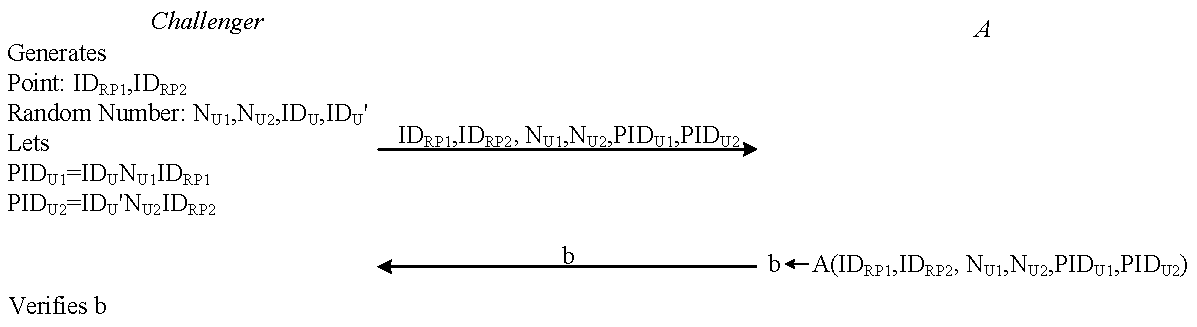
\includegraphics[width=0.82\linewidth]{fig/game1.pdf}
%  \caption{The Game.}
%  \label{fig:game}
%\end{figure*}


In the RP-based identity linkage,
    two RPs bring two triads received in SSO login instances, $\{ID_{RP_j}$, $t_j$, $[ID_U][t_j]{ID_{RP_j}}\}$ and
    $\{ID_{RP_{j'}}$, $t_{j'}$, $[ID_{U'}] [t_{j'}] {ID_{RP_{j'}}}\}$.
We describe the attack as the following game $\mathcal{G}$ between an adversary and a challenger:
    the adversary receives $\{ID_{RP_j}$, $t_j$, $[ID_U][t_j]{ID_{RP_j}}, ID_{RP_{j'}}$, $t_{j'}$, $[ID_{U'}] [t_{j'}] {ID_{RP_{j'}}}\}$ from the challenger,
     and outputs the result $s$.
The result is 1, when the adversary guesses that $ID_U = ID_{U'}$;
     otherwise, the adversary thinks they are different users (i.e., $ID_U \neq ID_{U'}$) and $s=0$.
%The game is shown as Figure \ref{fig:game}.

We define $Pr_c$ as the probability that
    the adversary outputs $s=1$ when $ID_U = ID_{U'}$ (i.e., a \emph{correct} identity linkage),
    and $Pr_{\bar{c}}$ as the probability that $s=1$ but $ID_U \neq ID_{U'}$ (i.e., an \emph{incorrect} result).
The successful RP-based identity linkage means
    the adversary has non-negligible advantages in $\mathcal{G}$.

\begin{figure}[tb]
  \centering
  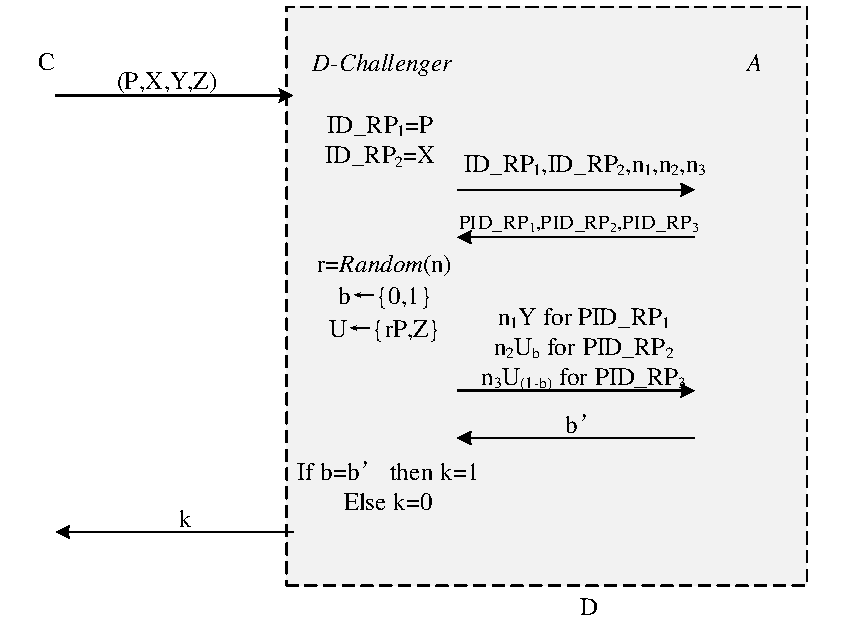
\includegraphics[width=0.95\linewidth]{fig/dalgorithm.pdf}
  \caption{The algorithm based on the RP-based identity linkage, to solve the ECDDH problem.}
  \label{fig:dalgorithm}
\end{figure}

We design a PPT algorithm $\mathcal{D}^*$ based on $\mathcal{G}$, shown in Figure \ref{fig:dalgorithm}.
The input of $\mathcal{D}^*$ is in the form of $\{Q_1, Q_2, Q_3, Q_4\}$, and each $Q_i$ is a point on $\mathbb{E}$.
On receiving the input,
 the challenger of $\mathcal{G}$ randomly chooses $t_j$ and $t_{j'}$ in $(1,n)$,
   % and sets $ID_{RP_j}=Q_1$, $ID_{RP_{j'}}=Q_2$, $PID_{U,j}=[t_j]Q_3$, and $PID_{U',j'}= [t_{j'}] Q_4$.
    and sends $\{Q_1, t_j, [t_j]Q_3, Q_2, t_{j'}, [t_{j'}] Q_4\}$ to the adversary in $\mathcal{G}$.
Finally,
    it directly outputs $s$ from $\mathcal{G}$ as the result of $\mathcal{D}^*$.

Let ($P$, $[x]P$, $[y]P$, $[xy]P$) and  ($P$, $[x]P$, $[y]P$, $[z]P$) be two inputs of $\mathcal{D}^*$.
Thus, we obtain
\begin{equation}\label{eq:game-succed}
\begin{split}
&Pr\{\mathcal{D}^*(P,[x]P,[y]P,[xy]P)=1\}\\
=&Pr\{\mathcal{G}(P, t_j, [t_j][y]P, [x]P, t_{j'},[t_{j'}][xy]P)=1\}\\
=&Pr\{\mathcal{G}(P, t_j, [y][t_j]P, [x]P, t_{j'},[y][t_{j'}][x]P)=1\}=Pr_c
\end{split}
\end{equation}
\begin{equation}\label{eq:game-fail}
\begin{split}
&Pr\{\mathcal{D}^*(P,[x]P,[y]P,[z]P)=1\} \\
=&Pr\{\mathcal{G}(P, t_j, [t_j][y]P, [x]P, t_{j'},[t_{j'}][z/x] [x]P)=1\}\\
=&Pr\{\mathcal{G}(P, t_j, [y][t_j]P, [x]P, t_{j'},[z/x][t_{j'}][x]P)=1\}=Pr_{\bar{c}}
\end{split}
\end{equation}
Equation \ref{eq:game-succed} is equal to $Pr_c$
        because it represents the correct case of $ID_{U} = ID_{U'} = y$,
 while Equation \ref{eq:game-fail} is $Pr_{\bar{c}}$ for it represents the incorrect case of $ID_{U} =y$ but $ID_{U'} = z/x \bmod n$.


The adversary has non-negligible advantages in $\mathcal{G}$ means
    $Pr_c - Pr_{\bar{c}}$ is non-negligible,
    and then $\mathcal{D}^*$ significantly distinguishes ($P$, $[x]P$, $[y]P$, $[xy]P$) from  ($P$, $[x]P$, $[y]P$, $[z]P$),
    which violates the ECDDH assumption.
So the adversary has no advantages in the game,
    and the RP-based identity linkage is computationally impossible in UPPRESSO.

%\section{Implementation and Evaluation}
\label{sec:implementation}
We have implemented the UPPRESSO prototype system, and experimentally evaluated its performance
 by comparing it with two open-source systems:
  (\emph{a}) MITREid Connect \cite{MITREid}
    which implements the PPID-enhanced OIDC protocol and prevents the RP-based identity linkage only,
     and (\emph{b}) SPRESSO \cite{SPRESSO} which only prevents the IdP-based login tracing.

\subsection{Prototype}
First of all, three identity-transformation functions are defined over
        the NIST P256 elliptic curve.
%randomly choose a 2048-bit prime as $p$, a 256-bit prime as $q$, and the  $q$-order generators as $ID_{RP}$.
%$N_U$ and $ID_U$  are 256-bit random numbers.
%Then, the discrete logarithm problem provides equivalent security strength (i.e., 112 bits) as RSA-2048 \cite{barkerecommendation}.
RSA-2048 and SHA-256 are adopted as the signature algorithm and the hash function, respectively.
%in  the $Cert_{RP}$, identity token and RP identifier refreshing result.

The IdP is built on top of MITREid Connect \cite{MITREid},
    an open-source OIDC Java implementation, %certificated by the OpenID Foundation \cite{OIDF},
    and only small modifications are needed as follows.
We add only 3 lines of Java code to calculate $PID_U$,
     about 20 lines to modify the way to send identity tokens,
    and about 50 lines in the function of RP Dynamic Registration to support the step of $PID_{RP}$ registration
            (i.e., checking $PID_{RP}$ and signing the registration result).
The calculations of $ID_{RP}$, $PID_U$, and RSA signature are implemented based on built-in Java cryptographic libraries. %(e.g., BigInteger).

We implemented the user-side functions by scripts downloaded from the IdP and RPs,
     containing about 200 and 150 lines of JavaScript code, respectively.
%to provide the functions in Steps 2.1, 2.3, and 4.3.
The cryptographic computations, e.g., $Cert_{RP}$ verification and $PID_{RP}$ negotiation, are implemented based on jsrsasign \cite{jsrsasign}, an efficient JavaScript cryptographic library.
%This chrome extension requires permissions  \emph{chrome.tabs} and \emph{chrome.windows} to obtain the RP's URL from the browser's tab,  and \emph{chrome.webRequest} to intercept, block, modify requests to the IdP or RP \cite{chromeExtension}.

%send HTTPS request/reply and hijack the HTTPS responses, to obtain the RP's URL and communicate with IdP and RP.
%and 30 lines  Chrome extension configuration files (specifying the required permissions, such as reading chrome tab information, sending the HTTP request, blocking the received HTTP response). to access to privileged fields of the Tab objects including

%Here, the cross-origin HTTPS requests sent by this chrome extension to the RP and IdP, will be blocked by Chrome due to the default same-origin security policy.
%To avoid this block, UPPRESSO modifies the IdP and RP, and sets \verb+chrome-extension://chrome-id+ (\verb+chrome-id+ is uniquely assigned by Google) in \verb+Access-Control-Allow-Origin+ header of the IdP's and RP's responses.

%Moreover, the chrome extension needs to construct cross-origin requests to communicate with the RP and IdP, which is forbidden by the default same-origin security policy. Therefore it is required to add the HTTP header \verb+Access-Control-Allow-Origin+ in the response of IdP and RP to accept only the request from the origin \verb+chrome-extension://chrome-id+ (\verb+chrome-id+ is uniquely assigned by the Google).

We provide a Java SDK for RPs in UPPRESSO.
The SDK provides two functions to encapsulate the protocol steps:
 one to request identity tokens,
    and the other to derive the accounts from identity tokens.
The SDK is implemented based on the Spring Boot framework  with about 1,000 lines of Java code
 and cryptographic computations are implemented based on the Spring Security library.
An RP invokes these two functions for the integration,
    by less than 10 lines of Java code.

%RP processing login request containing  and identity token parsing containing $Account$ calculation in Figure \ref{fig:process}.


%\subsection{Performance Evaluation}
\label{sec:evaluation}
\textcolor{red}{Three machines connected in an isolated 1Gbps LAN,
    build the experimental SSO environment.
The CPUs are Intel Core i7-4770 3.4 GHz for the IdP,
    Intel Core i7-4770S 3.1 GHz for the RP, and Intel Core i5-4210H 2.9 GHz for users.
Each machine is configured with 8 GB RAM and
    installs Windows 10 as the operating system.
The user agent is Chrome v75.0.3770.100.}

%RP���������ض�������SDK����Լ��Ҫ230��JAVA����
%OIDC��MITREid����SDK��Ҫ��Լ20�е�JAVA���룬��Ҫ��������һ��HTML�ļ���������Լ20��JavaScript���룩
%UPPRESSO��SDK��Ҫ��Լ1100�д��룬����Ҫ���Ӷ����HTML�ļ�
%OIDC��UPPRESSO��SDKֻ��ҪRP�ṩ��������ӿڣ���ַ����Ȼ���ڶ�Ӧ������ӿ������ö�Ӧ��API��ÿ���ӿڶ�Ӧһ��API���ֱ�����ΪtokenRequestGenerate��userAccountAchieve���������Ĵ������̾���SDK���
%SPRESSO���ڽṹ��OIDC��ȫ��ͬ������ʹ����SPRESSO�ṩ��RP�Ŀ�Դ����
%For better evaluation, we build one RP for both UPPRESSO and MITREid Connect which is also implemented  based on Spring Boot framework, as well as the identity token transmission from user to RP in MITREid Connect is implemented by JavaScript running in RP's web page. The IdP in MITREid Connect is achieved from github \cite{MITREid}. However, the SPRESSO system is downloaded from \cite{spressome} containing IdP, RP and FWD.

%A DELL OptiPlex 9020 PC (Intel Core i7-4770 CPU, 3.4GHz, 500GB SSD and 8GB RAM) with Window 10 prox64 works as the IdP. A ThinkCentre M9350z-D109 PC (Intel Core i7-4770s CPU, 3.1GHz, 128GB SSD and 8GB RAM) with  Window 10 prox64 servers as RP. The user adopts Chrome v75.0.3770.100 as the user agent on the Acer VN7-591G-51SS Laptop (Intel Core i5-4210H CPU, 2.9GHz, 128GB SSD and 8GB RAM) with  Windows 10 prox64. For SPRESSO, the extra trusted entity FWD is deployed on the same machine as IdP.
%û����Ϊ������ͬһ��������ʹ�ÿ����䳤��monitorָϵͳ�ļ�����
%The monitor demonstrates that the calculation and network processing of the IdP does not become a bottleneck (the load of CPU and network is in the moderate level).

We compared UPPRESSO with MITREid Connect and SPRESSO.
%In the evaluation,
    MITREid Connect runs with the standard implicit login flow of OIDC,
 while the identity tokens in SPRESSO are also forwarded by a user to the RP,
    similarly to the implicit flow. %to some extent.
In the identity tokens of SPRESSO, $PID_{RP}$ is the encrypted RP domain, while the one-time symmetric key only known by the RP and the user.
They also configure RSA-2048 and SHA-256  in the generation of identity tokens.


MITREid Connect provides open-source Java implementations of IdP and
RP SDK,
 while SPRESSO implements all entities by JavaScript based on node.js.
We implemented the RPs based on Spring Boot for UPPRESSO and MITREid Connect, by integrating the corresponding SDKs.
The RPs in three schemes provide the same function, i.e.,
     simply extract the user's account from verified identity tokens.

We measured the time for a user to login to an RP
     and calculated the average of $1,000$ measurements.
We divide a login flow into three parts:
{\em Preparation and identity-token requesting} (for UPPRESSO, it includes Steps 1-2 in Figure \ref{fig:process}),
  to construct an identity-token request transmitted to the IdP;
{\em Identity-token generation} (Step 3 in Figure \ref{fig:process}),
    for the IdP to generate an identity token (while the user authentication is not included);
and {\em Identity-token acceptance} (Step 4 in Figure \ref{fig:process}),
    as the RP receives, verifies and parses the identity token.
% and \textbf{Identity token verification} (Steps 5.1 and 5.2 in Figure \ref{fig:process}), the RP verifying and parsing the identity token.



\begin{figure}[tb]
  \centering
  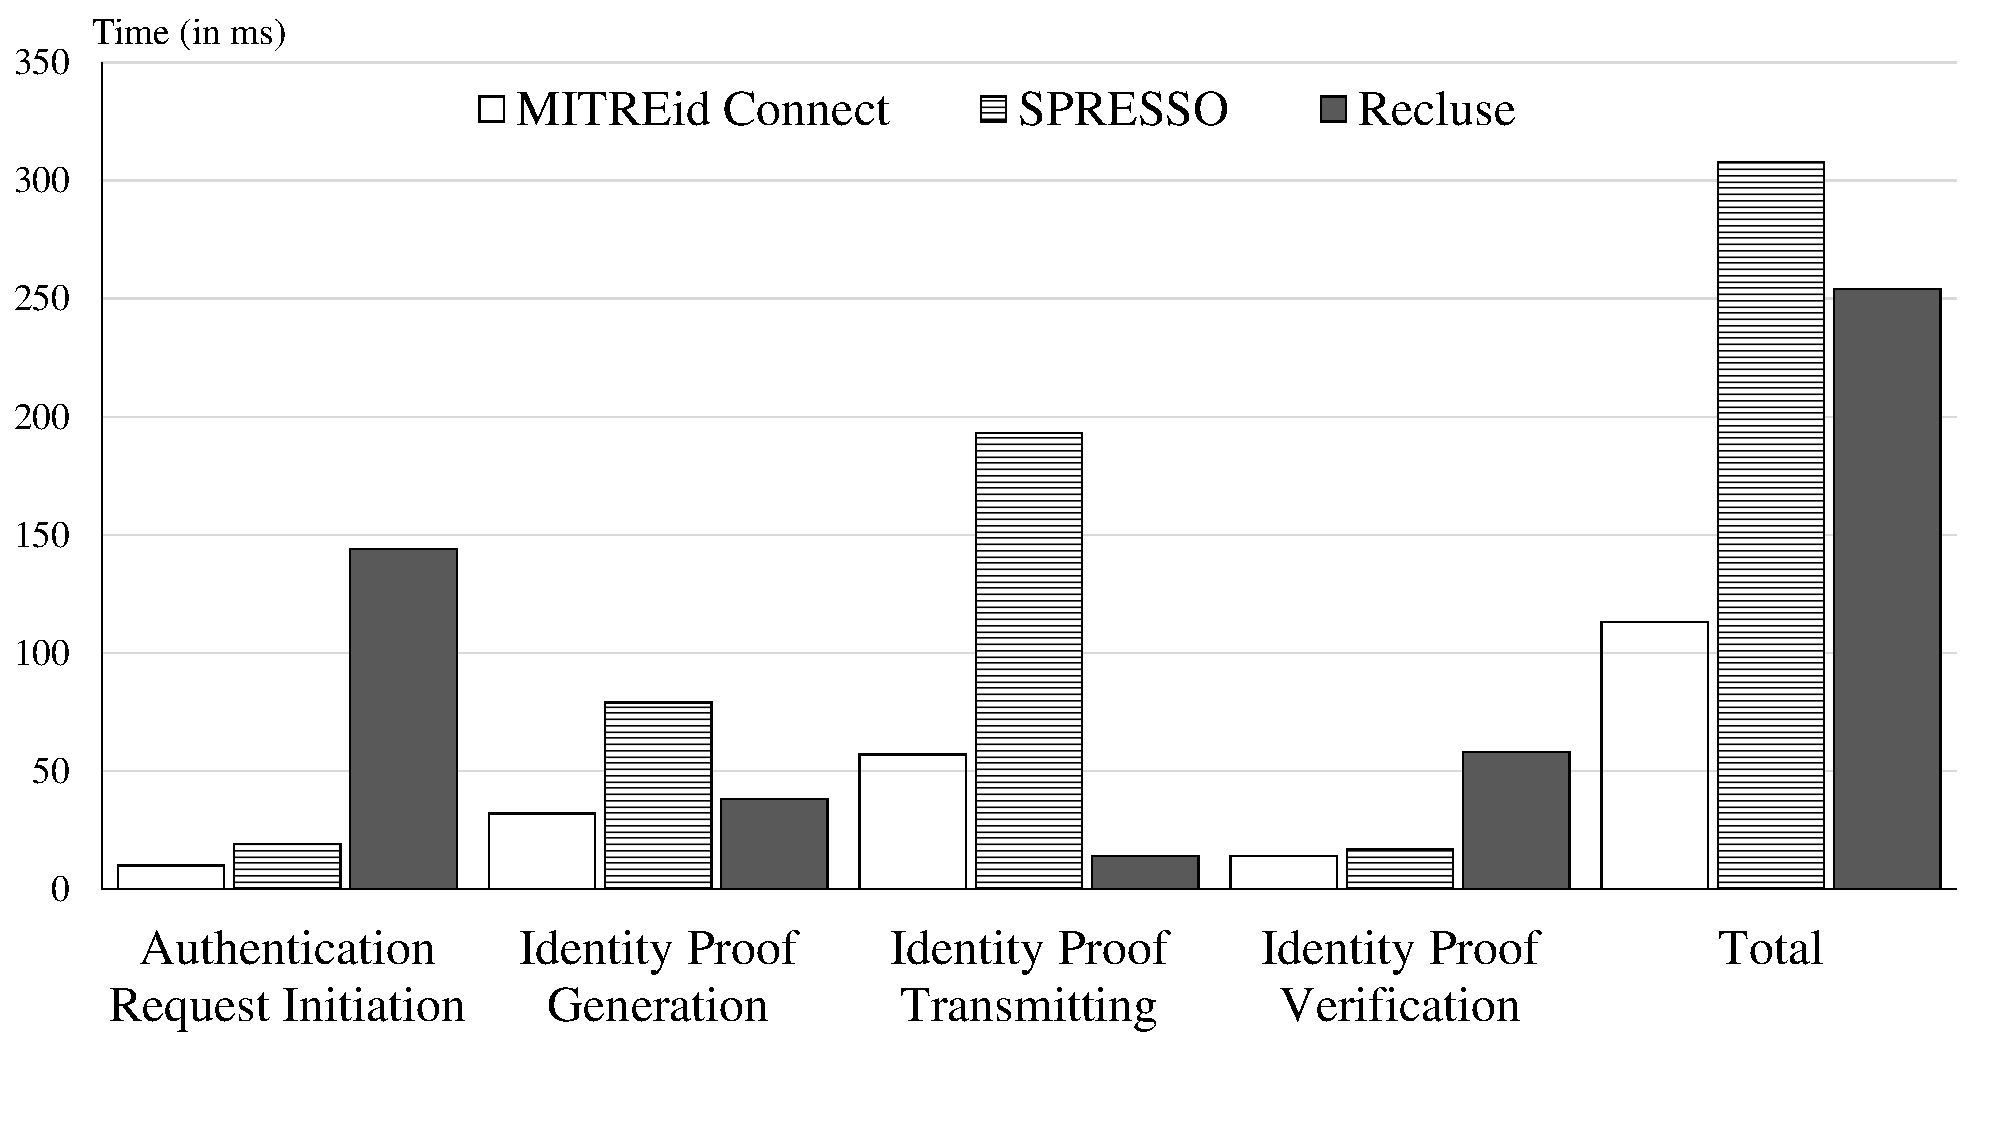
\includegraphics[width=0.94\linewidth]{fig/evaluation2.pdf}
  \caption{The time cost of SSO login.}
  \label{fig:evaluation}
\end{figure}

The results are shown in Figure \ref{fig:evaluation}.
The overall times of SSO login are  113 ms, 310 ms, and 308 ms for MITREid Connect, UPPRESSO, and SPRESSO, respectively.

In the preparation and identity-token requesting, MITREid Connect only needs 10 ms but
    UPPRESSO requires 271 ms.
The main overhead in UPPRESSO is to open the new browser window and download the scripts, which needs about 104 ms.
This overhead can be mitigated by silently conducting these operations when the user visits the RP website,
    or by the implementation with browser extensions.
SPRESSO needs 19 ms in the preparation and identity-token requesting,
    a little more than MITREid Connect,
for an RP to obtain some information on the IdP  % 's public key %(SPRESSO allows a user to assign any IdPs before login without initial registrations)
     and encrypt its domain using an ephemeral symmetric key.



%�����ܼ��ٶ��٣�
In the identity-token generation,
     UPPRESSO needs 34 ms.
Compared with MITREid Connect,
    it needs 2 more ms to calculate  $PID_U$.
SPRESSO requires 71 ms to generate an identity token,
    as it implements the IdP based on node.js and therefore adopts a JavaScript cryptographic library,
 while a more efficient Java library is used in others.
%As the processings in SPRESSO and MITREid Connect are the same, the processing time in SPRESSO may be reduced to 32 ms.
%And, then the overall time in SPRESSO will be 269 ms, still larger than 254 ms in UPPRESSO.

%transmission & extraction
In the identity-token acceptance,
 UPPRESSO only needs about 6 ms for the scripts to send an identity token to the RP,
    which verifies it and calculates $Acct$.
It takes 71 ms for MITREid Connect to accept this identity token:
    when the token is redirected to the RP,
        it must be carried within an URL following  the fragment identifier \verb+#+ instead of \verb+?+,
         due to some security considerations \cite{de2014oauth},
        so the identity token has to be sent to the RP by JavaScript functions (but not HTTP requests)
            and most time is spent to download the script from the RP.
SPRESSO needs the longest time (210 ms) due to the complicated process at the user browser:
        after receiving identity tokens from the IdP,
        the browser downloads the JavaScript program from a trusted forwarder,
            decrypts the RP endpoint, and finally sends identity tokens to this endpoint.
%In the evaluation, the forwarder and IdP are deployed in one machine, which doesn't introduce performance degradation based on the observation. % as  FWD and IdP work sequently for one login.

%SPRESSO needs a trusted entity named FWD for transmitting the identity token. We deployed FWD and IdP on the same machine to reduce transmitting delay between them, while the computation never becomes the bottleneck according to the observation.


%In the verification, UPPRESSO needs an extra calculation for $Account$, which then requires  58 ms,
% compared to 14 ms in MITREid Connect and 17 ms in SPRESSO.

%\section{Discussions}
\label{sec:discussion}

\noindent{\textbf{IdP-RP collusive attacks.}}
Privacy-preserving identity federation solutions \cite{ELPASSO, UnlimitID, idemix, PseudoID, Opaak, uprov}
 prevent collusive attacks by an IdP and RPs,
 but require (\emph{a}) a long-term secret held by a user and verified by RPs
  and (\emph{b}) user-managed accounts for different RPs.
These accounts may be derived from an RP's domain and the user's secret \cite{ELPASSO, UnlimitID, Opaak, uprov,idemix},
 but still bring inconvenience to users as below.
For web applications, users need to install a browser extension to handle this long-term secret.
If it is lost or leaked, the user must notify all RPs to update her accounts derived from this secret.
Note that if the accounts are not masked by the user secret, the colluding IdP and RPs can eventually link them.
Unlike these approaches, \usso\ does not protect user privacy against such collusive attacks,
 because a user is authenticated only \emph{once} in the login flow.
 The user's identity at the IdP is transformed into accounts at RPs,
  which are unrelated to any user credentials such as passwords, one-time passwords, smart cards, or FIDO devices.

%\vspace{0.75mm}
\noindent \textbf{Scalability.} $ID_{RP}$ is generated uniquely during the initial registration of an RP,
 with a capacity of $n$, which is the order of $G$. For the NIST P256 elliptic curve, $n$ is approximately $2^{256}$.
$PID_{RP}$ is ensured to be unique in unexpired tokens.
The probability of having at least two identical $PID_{RP}$s among $\sigma$ unexpired tokens is $1-\prod_{i=0}^{\sigma-1}(1-i/n)$.
If the system serves $10^{8}$ requests per second and has a validity period of 10 minutes, $\sigma$ is less than $2^{36}$,
 and the $PID_{RP}$-collision probability is negligible, i.e., less than $2^{-183}$ for the NIST P256 curve.

The capacity of accounts at any RP is the same as the capacity of user identities at the IdP,
 which is also $n$. Since $\mathbb{E}$ is a finite cyclic group, $ID_{RP} = [r]G$ is also a generator of order $n$.
 Therefore, for any RP, a unique account is automatically assigned to every user because $Acct =  [ID_U]ID_{RP} = [u]ID_{RP}$.
In addition, stronger elliptic curves accommodate more RPs and users, e.g., $n$ is about $2^{384}$ for the NIST P384 curve.


%\vspace{0.75mm}
\noindent \textbf{Alternative methods for generating $ID_{RP}$ and binding $Enpt_{RP}$.}
In \usso\ the IdP generates random $ID_{RP}$ and uses an RP certificate to bind $ID_{RP}$ and $Enpt_{RP}$, which is verified by the IdP script.
This ensures the target RP has already registered itself at the IdP and prevents unauthorized RPs from accessing the IdP's services.

An alternative method for binding $ID_{RP}$ and $Enpt_{RP}$ is
 to \emph{deterministically} calculate $ID_{RP}$ based on the RP's unambiguous name such as its domain.
 This can be achieved by encoding the domain using a hashing-to-elliptic-curves function \cite{irtf-cfrg-hash-to-curve-16},
  to generate a point on the elliptic curve $\mathbb{E}$ as $ID_{RP}$.
This function provides collision resistance
 and does not reveal the discrete logarithm of the output \cite{irtf-cfrg-hash-to-curve-16},
  ensuring the \emph{uniqueness} of $ID_{RP} = [r]G$ while keeping $r$ unknown. %For example, using a hash function $Hs()$ to encode an RP's domain or the RP script's origin, e.g., verb+https://RP.com+)

In this case, the RP script sends only the endpoint but not its RP certificate in Step 2.2, and the IdP script calculates $ID_{RP}$ by itself. %This elimination of RP certificates improves the downloading of scripts, and on average \textcolor[rgb]{1,0,0}{xxx} ms are saved.
However, if the RP changes its domain, such as from \verb+https://RP.com+ to \verb+https://theRP.com+,
$Acct = [ID_U]ID_{RP}$ will inevitably change.
This requires each user to explicitly perform special operations to migrate her account to the updated RP system.
It is worth noting that the user operations cannot be eliminated in the migration from an RP to the updated one;
otherwise, it implies two colluding RPs could link a user's accounts across these RPs.

\newc
%\vspace{0.75mm}
\noindent \textbf{Quantum-resistance.}
The current designs of \usso\ does not support quantum security.
In our future work, we will investigate alternative algorithms for quantum-secure services.
We plan to adopt a quantum-resistant public-key algorithm, for the IdP to sign identity tokens and RP certificates.
Moreover, we will study existing quantum-secure ORPF protocols \cite{ideal-lattice-oprf,isogency-oprf}
 to see if they support RP designation.
As discussed in Section \ref{sec:related}, such OPRF designs can be utilized to implement the \usso\ protocol.

%To build quantum-secure SSO services with the \usso\ protocol, an IdP needs to generate a key pair of quantum-resistant public-key algorithms for signing identity tokens and RP certificates. Moreover, as discussed in Section \ref{sec:related}, \usso\ leverages the OPRF design \cite{oprf-proved,voprf-proved} in identity transformations for privacy-preserving SSO. To support RP designation, it requires that no collision exists in the blinded inputs of the evaluated pseudo-random function. In our future work, we will study if existing quantum-secure ORPF protocols \cite{ideal-lattice-oprf,isogency-oprf} support this property.
%to find out whether they can work for the quantum-secure identity transformations in \usso.

\oldc

%\vspace{0.75mm}
\noindent \textbf{Restriction of the RP script's origin.}
When the IdP script forwards identity tokens to the RP script, the \verb+postMessage+ targetOrigin mechanism \cite{postm-targeto} is used to restrict the recipient of the tokens, to ensure that the tokens will be sent to the intended $Enpt_{RP}$, as specified in the RP certificate. The targetOrigin is specified as a combination of protocol, port (if not present, 80 for \verb+http+ and 443 for \verb+https+), and domain (e.g., \verb+RP.com+).
The RP script's origin must accurately match the targetOrigin to receive the tokens.

Although it does not check the URL path in $Enpt_{RP}$,
the targetOrigin mechanism introduces no {\em additional} risk.
%This assumes only one RP runs on a domain.
For example, if two RPs run on the same domain with different endpoints to receive tokens,
 e.g., \verb+https://RP.com/honest/tk+ and \verb+https://RP.com/malicious/tk+,
  they cannot be distinguished by \verb+postMessage+ when the IdP script is sending tokens.
Since browsers control access to web resources with the same-origin policy (SOP) \cite{sop},
   an RP's resources in browsers could still be accessed maliciously by the other RP running on the same domain,
    such as stealing cookies using the script \verb+window.open('https://RP.com/honest').document.cookie+,
even if it restricts that only HTTP requests to specific paths carry its cookies.
 This risk actually arises from the SOP design of browsers, but not the \usso\ protocol.

%\vspace{0.75mm}
\noindent \textbf{Support for the authorization code flow.} In OIDC authorization code flow \cite{OpenIDConnect},
 the IdP does not directly provide identity tokens.
 Instead, it sends an authorization code to the RP, which uses this code to request identity tokens.
 The identity-transformation algorithms, namely $\mathcal{F}_{PID_{U}}$, $\mathcal{F}_{PID_{RP}}$, and $\mathcal{F}_{Acct}$,
  can be integrated into this flow as below. %similar to the login flow introduced in Section \ref{implementations},

The IdP script can forward an authorization code to the RP script,
 and then to the RP. %that binds $PID_U$ and $PID_{RP}$.
 An authorization code only serves as an index to retrieve identity tokens from the IdP
  and does not reveal any information about the authenticated user.
After receiving an authorization code,
 an RP uses it along with a secret credential issued by the IdP during the initial registration \cite{OpenIDConnect}
  to retrieve identity tokens from the IdP.
  However, to protect the RP identities from the IdP, privacy-preserving tokens
   (e.g., ring or group signatures \cite{ring-sig,chaum1991group} and TrustToken \cite{trusttoken})
   and anonymous networks (e.g., Tor \cite{tor}) need to be adopted for RPs in the retrieval of identity tokens.



%\vspace{0.75mm}
\noindent \textbf{Applicability of identity transformations.}
The proposed identity-transformation algorithms %i.e., $\mathcal{F}_{PID_{RP}}()$, $\mathcal{F}_{PID_U}()$, and $\mathcal{F}_{Acct}()$,
can be applied to a wide range of SSO scenarios, including web applications, mobile Apps, and native software.
These algorithms follow the common model of popular SSO protocols and do not depend on any specific implementation or runtime.%, making them highly versatile and adaptable to different use cases.

%%%%%%%%%%%%%%%%%%%%% 几个方面的扩展
% 1. 解决IdP数据泄露
% 如果IdP的数据库泄露,用户列表u公开,则RP就可以,针对每一个u,计算[u]ID_{RP};然后,
% 2. 授权码模式
% 可以使用PKCE方式,直接在前端获取。通常,PKCS模式用在没有后端的RP(例如,纯客户端)。
% 对于有后端,可以将​code_verifier传给RP后端?也能够达到目标。
% 3. RP后端访问IdP,需要通过TOR
% 为了不传递RP ID和Secret,可以是:传递PKCE的code_verifier [user将code_verifier传递给RP],
% 也可以是群签名/环签名之类的。
% 4. 要求RP有授权
% 可以有2种方式:
%   去掉RP Cert;采取授权码方式 + 群签名/环签名之类凭证。
%   去掉RP Cert:采取授权码方式 + PrivacyPass之类匿名凭证(还可以有准确计费)。
% 5. 还有一种方式
% 隐式模式 + PrivacyPass之类匿名凭证(还可以有准确计费)。因为其它方式都需要通过TOR。

%\subsection{Extended Related Works}
\label{sec:related}

%Such tokens (or credentials) authorize a user to conduct operations
%        in privacy-preserving ways.
%
%    tokens (or credentials) authorize a user to conduct operations
%        in privacy-preserving ways.
%Privacy-enhancing technologies have been applied in various scenarios,
%  but not adopted to comprehensively transform the five (pseudo-)identities in SSO services.

\newc
\noindent\textbf{Privacy-preserving cryptographic techniques.}
PrivacyPass and TrustToken \cite{privacypass,trusttoken} propose anonymous tokens for applications that grant anonymous access to authorized users. They used a cryptographic technique that was originally designed for oblivious pseudorandom functions (OPRFs) \cite{oprf-proved,voprf-proved}. 
A user generates a random number $e_i$ for each unsigned token $T_i$ and blinds $T_i$ into $T_i^{e_i}$. After the user is authenticated, a token server signs ($T_i^{e_i}, T_i^{e_i k}$) with a private key $k$. Then, the user converts $T_i^{e_i k}$ to $T_i^k$ using $e_i$ and redeems the token ($T_i, T_i^k$) to access resources. 
%the token server blindly binds user-selected secrets $t_i$ and access tokens ($T_i, T_i^{k{r_i}}$) and signs them with its secret key $k$, where $T_i=H(t_i)$ and $H$ is a hash function.
%The user unblinds them to obtain anonymous tokens ($t_i, T_i^k$) and redeems them later on the service.
%The random numbers (or blinding factors) prevent the token server from linking token signing and redemption. 
Anonymous tokens may be used to build anonymous SSO services, where an RP cannot identify the users. 
% they can be used to implement anonymous SSO services that are secure against IdP-based tracing and RP-based linkage.}
%\textcolor{blue}{They provide SSO services that are fundamentally different from the ones offered by UPPRESSO. As shown in Table~\ref{tbl:comparison-protocol}, they lack support for all three SSO features. First, the anonymous tokens used by different users or by the same user in different login instances cannot be distinguished (i.e., no user identification at RPs), since they are signed blindly using the same server secret. Besides, the users are required to maintain anonymous tokens for asynchronous authentication in addition to the credentials for the IdP, similar to other privacy-preserving solutions based on anonymous credentials. Finally, PrivacyPass and TrustToken do not support selective user attribution provisioning. In contrast, UPPRESSO formalizes the privacy-preserving SSO process as two ID-transformation problems and generates unlinkable pseudoidentities and proofs to support the desired SSO features. Therefore,  UPPRESSO is  compatible with widely-adopted SSO protocols such as OIDC and SAML.}
%\textcolor{blue}{PrivacyPass and TrustToken allow a user to receive tokens \cite{privacypass,trusttoken}, each of which is denoted as ($T, T^{k}$), where $k$ is the token server's private key. These tokens are used to access resources anonymously in the future. To unlink token signing and redemption, a user generates a random number $e$ for each token, blinds $T$ into $T^{e}$, and sends it to request ($T^e, T^{ek}$) from the token server. The user then utilizes $e$ to obtain $T^k$ from $T^{ek}$, and then only ($T, T^{k}$) is redeemed to access resources. This cryptographic skill \cite{oprf-proved} is used in UPPRESSO similarly: a user transforms $ID_{RP}$ to $PID_{RP} = [t]ID_{RP}$ by a random number $t$, and $PID_{RP}$ is transformed again by an IdP to $[tu]ID_{RP}$. The visited RP calculates $Acct = [u]ID_{RP}$ from $[tu]ID_{RP}$ by using $t$ (see Table \ref{tbl:notations-protocol} for detailed descriptions of these notations).}
\usso's identity transformations are implemented using a similar cryptographic technique. In particular, a user first transforms $ID_{RP}$ to $PID_{RP} = [t]ID_{RP}$ using a random number $t$, and then the IdP transforms $PID_{RP}$ further to $[tu]ID_{RP}$. The visited RP finally calculates $Acct = [u]ID_{RP}$ from $[tu]ID_{RP}$ by using $t$.
 %(see Table \ref{tbl:notations-protocol} for detailed descriptions of these notations).
% \textcolor{blue}{UPPRESSO differs from PrivacyPass and TrustToken as below.
% Firstly, PrivacyPass and TrustToken work as anonymous SSO to some extent, where one consistent private key serves all users, but UPPRESSO identifies each user at an RP. Secondly, the above cryptographic skill \cite{oprf-proved} is differently utilized. UPPRESSO integrates it to transform identities in SSO:
Here, \usso~supports the IdP-untraceability property that prevents the IdP from linking $ID_{RP}$ and a corresponding $[t]ID_{RP}$, leveraging the ECDLP assumption (see Section~\ref{analysis-security}). This is similar to the unlinkability between token signing and redemption in PrivacyPass/TrustToken, which prevents the server from linking ($T_i^{e_i}, T_i^{e_ik}$) and  ($T_i, T_i^k$), leveraging the DLP assumption. %The unlinkability between token signing and redemption, or ($T_i^{e_i}, T_i^{e_ik}$) and  ($T_i, T_i^k$), roughly corresponds to only the IdP-untraceability in UPPRESSO: an IdP cannot link any pair of $[t_i]ID_{RP}$ and $ID_{RP}$.  % $i = 1, 2, \cdots$. % which fundamentally depends on the ECDLP assumption.

However, \usso~explores this cryptographic technique %with different designs and 
in greater depth, resulting in additional privacy property that is not considered or supported in existing anonymous tokens \cite{privacypass,trusttoken}. %or OPRFs \cite{oprf-proved,voprf-proved}
The exponent $k$ in PrivacyPass/TrustToken is held only by the server as a private key, and the random number $e$ is only known to a user. In contrast, the scalar $u$ in \usso~denotes a user identity known to the user and the IdP, while the random number $t$ is an ephemeral secret shared between the user and the RP.  
%The application of the cryptographic technique differs from PrivacyPass/TrustToken
%This different design allows \usso~to explore and offer additional privacy properties. %Furthermore, more privacy properties are explored in UPPRESSO.
The sharing of random numbers supports additional unlinkability across colluding RPs. Their knowledge about two different users $u$ and $u'$, i.e., ($ID_{RP}, t, [u]ID_{RP}$) and ($ID_{RP'}, t', [u']ID_{RP'}$), which is obtained from different logins, are indistinguishable. 
%given multiple users, e.g., identified as $u$ and $u'$, ($ID_{RP}, t, [u]ID_{RP}$) and ($ID_{RP'}, t', [u']ID_{RP'}$) are indistinguishable to colluding RPs.
This property requires designing the transformations under not only ECDLP but also ECDDH assumptions (see Section~\ref{sec-:analysis}).

% \noindent\textbf{Anonymous SSO.}
% Such schemes allow authenticated users to access a service protected by an IdP,
%     without revealing their identities.
% Anonymous SSO was proposed for GSM communications \cite{ElmuftiWRR08},
%     and formalized \cite{WangWS13}.
% Privacy-preserving primitives, such as group signature, zero-knowledge proof, Chebyshev Chaotic Maps and proxy re-verification,
%      were adopted to design anonymous SSO \cite{WangWS13,HanCSTW18,Lee18,HanCSTWW20}.
% Anonymous SSO schemes work for some special applications,
%     but are unapplicable in most systems that require user identification for customized services.

\oldc
Various cryptographic primitives have been used to protect user privacy.
Using zero-knowledge proofs, ZKlaims \cite{zklaim} allows users to prove statements on the credentials issued by a trusted server without revealing the credential contents.
Crypto-Book \cite{crypto-book} adopts distributed key generation to generate linkable-ring-signature private keys for users, and each key pair is used as an untraceable pseudonym. Tandem \cite{tandem} generates one-time-use key-share tokens for a two-party threshold cryptographic scheme implemented with a central server to protect the privacy of key-usage patterns.


%two-party threshold cryptographic scheme implemented with a central server, to protect user private keys \cite{mRSA,ss-rsa}: to sign/decrypt a message, a user needs a token from the server.
%    Tandem \cite{tandem} decouples the obtaining and using of such tokens, for the privacy of key usage.

%\vspace{0.5mm}
\noindent\textbf{Formal analysis of SSO protocols.}
A formal analysis on SAML-based SSO \cite{ArmandoCCCT08} found that a Google-implemented variant does not bind RP identities correctly in the identity tokens.
Fett et al. \cite{FettKS16, FettKS17} formally analyzed OAuth 2.0 and OIDC using a Dolev-Yao-style model \cite{FettKS14} and reported the 307 redirection and IdP mix-up attacks. In this paper, we also developed a Dolev-Yao-style model for \usso~to prove its security and privacy (see Section~\ref{dy-model}).


%\vspace{0.5mm}
\noindent\textbf{Implementation vulnerabilities in SSO.}
Various vulnerabilities have been found in several SSO systems for web applications, resulting in attacks %of impersonation and identity injection
that break the confidentiality \cite{WangCW12,ccsSunB12,ArmandoCCCPS13,DiscoveringJCS,dimvaLiM16}, integrity \cite{WangCW12,SomorovskyMSKJ12,WangZLG16,MainkaMS16, MainkaMSW17,dimvaLiM16} or RP designation \cite{WangZLG16,MainkaMS16,MainkaMSW17,YangLCZ18,dimvaLiM16} of identity tokens.
%In the SSO services of Google and Facebook, %from the view of browser-relayed traffics
%    logic flaws of the IdPs and RPs were detected \cite{WangCW12}.  % to break the confidentiality and integrity of identity tokens.
The integrity of identity tokens was violated %\cite{SomorovskyMSKJ12,WangCW12,WangZLG16,MainkaMS16, MainkaMSW17}
due to software flaws such as defective verification by RPs \cite{WangCW12,WangZLG16,MainkaMSW17}, XML signature wrapping \cite{SomorovskyMSKJ12}, and IdP spoofing \cite{MainkaMS16,MainkaMSW17}.
Meanwhile, the RP designation was broken because of incorrect binding by an IdP \cite{YangLCZ18,WangZLG16} or insufficient verification by RPs \cite{MainkaMS16,MainkaMSW17,YangLCZ18}.
A defective IdP does not always enclose an identifiable Email address in tokens \cite{WangCW12},
 which breaks the user identification.
Similar vulnerabilities have been found in Android Apps that break the confidentiality \cite{ChenPCTKT14,WangZLLYLG15,YangLS17,ShiWL19}, integrity \cite{ChenPCTKT14,YangLS17}, and RP designation \cite{ChenPCTKT14,ShiWL19,WangZLLYLG15} of SSO identity tokens.

%Navas et al. \cite{NavasB19} discussed the possible attack patterns against OIDC services.
%Automatic tools such as SSOScan \cite{ZhouE14}, OAuthTester \cite{YangLLZH16} and S3KVetter \cite{YangLCZ18},
% detect the violations of confidentiality, integrity, or RP designation of SSO identity tokens.
% Wang et al. \cite{ExplicatingSDK} detect the vulnerable applications
%     built with authentication/authorization SDKs,
%      due to the implicit but unsuitable assumptions of these SDKs.


%Furthermore, if a user is compromised, the attacker can login to RPs on his behalf. So, we consider malicious users, malicious RPs, and colluding users and RPs in our threat model (see Section~\ref{subsec:threatmodel}).





% In a mobile system,
% browsers, IdP Apps,
%     or IdP-provided SDKs %(e.g., an encapsulated WebView)
%          are responsible for forwarding identity tokens, %from the IdP App to RP Apps.
% but none of them ensures an identity token is sent to the designated RP only \cite{ChenPCTKT14,WangZLLYLG15}.
% %    because a WebView or the system browser cannot authenticate the RP Apps and the IdP App may be repackaged.
% %SSO protocols are modified for mobile Apps, but the modifications are not well understood by developers \cite{ChenPCTKT14,YangLS17}.
% Vulnerabilities were found in Android Apps,
%     to break confidentiality \cite{ChenPCTKT14,WangZLLYLG15,YangLS17,ShiWL19}, integrity \cite{ChenPCTKT14,YangLS17}, and RP designation \cite{ChenPCTKT14,ShiWL19} of identity tokens.
% A flaw was found in Google Apps \cite{ArmandoCCCPS13}, allowing a malicious RP to hijack a user's authentication attempt and inject a payload to steal the cookie or identity token belonging to another RP.

% If a user is compromised,
%     attackers will login to RPs on behalf of him.
% Single sign-off helps the victim user
%  to revoke all his tokens accepted and logout from the RPs  \cite{GhasemisharifRC18}.
% FedCM \cite{FedCM} attempts to disable iframe and third-party cookies in SSO, which might be exploited to track users.
% %UPRRSSO protects privacy in SSO through ID transformations and our prototype does NOT use either iframe or third-party cookies.


%\section{Conclusion}
\label{sec:conclusion}
This paper presents \usso, an untraceable and unlinkable privacy-preserving SSO system for protecting a user's online profile across different RPs against both a curious IdP and colluding RPs.
We propose an identity-transformation approach for privacy-preserving SSO and design algorithms that satisfy the requirements, where (\emph{a}) $\mathcal{F}_{PID_{RP}}$ protects an RP's identity from the curious IdP, (\emph{b}) $\mathcal{F}_{PID_{U}}$ prevents colluding RPs from linking a user across different RPs, and (\emph{c}) $\mathcal{F}_{Acct}$ enables an RP to derive an identical account for a user in multiple logins. These identity transformations are integrated into the widely-adopted OIDC protocol, maintaining user convenience and security guarantees of SSO services. Our experimental evaluations of the \usso\ prototype demonstrate its efficiency, with an average login taking 174 ms when the IdP, the visited RP, and users are deployed in a virtual private cloud, or 421 ms when a user visits remotely.

%\section*{Acknowledgments}
%We would like to thank the anonymous shepherd and reviewers for their valuable comments.
%Prof. Xianhui Lu at Institute of Information Engineering, CAS and Mr. Wentian Zhu at School of Cyber Security, USTC
%    helped us to improve the analysis of security and privacy.


\bibliographystyle{IEEEbib}
\bibliography{ref}

\end{document}

%2020.2.6
%introdution ÖУ¬½²ÊöIdPºÍRPºÏı£¬arge IdPs, especially social IdPs like Google and Facebook
%introdution ÖУ¬We have implemented a prototype of UPPRESSO based on an open-source implementation of OIDC£¬½²Ï¶¯Ì¬×¢²á¡£
%3.A ÖÐReceiver designationÕâ¸ö´Ê£¨binding ºÍ userÈ·±£Ö»·¢¸ø¶ÔÓ¦RP£©¡£ integrityºÍconfidentity£¨HTTPS£©·ÅÔÚÒ»Æð¡£

%RPID renew---¡·refresh
